\documentclass{ipol}


\usepackage[utf8]{inputenc} % allow utf-8 input
\usepackage[T1]{fontenc}    % use 8-bit T1 fonts
\usepackage{hyperref}       % hyperlinks
\usepackage{url}            % simple URL typesetting
\usepackage{booktabs}       % professional-quality tables
\usepackage{amsfonts}       % blackboard math symbols
\usepackage{nicefrac}       % compact symbols for 1/2, etc.
\usepackage{microtype}      % microtypography
\usepackage{xcolor}         % colors

\usepackage{adjustbox}
% \usepackage[margin=2cm]{geometry}
\usepackage{amsmath}
\usepackage{amssymb}
\usepackage{amsthm}
\usepackage{tcolorbox}
\usepackage{amsfonts}
\usepackage{stmaryrd}
\usepackage{xcolor}
\usepackage{algpseudocode}
\usepackage{algorithm}
\usepackage{mathtools}
\usepackage{dsfont}
\usepackage{tikz}
\usepackage{tikz-cd}
\usepackage{bussproofs}
\usepackage{listings, lstautogobble}
\usepackage{caption}
\usepackage{subcaption}
\usepackage{graphicx}
\usepackage{svg}
\usepackage{float}
\usepackage{appendix}
\usepackage{natbib}
\bibliographystyle{plainnat}
%\usepackage[french]{babel}
\usepackage{multicol}
\usepackage{multirow}
\usepackage{tabularx}
\usepackage[percent]{overpic}
\usepackage{todonotes}
\usepackage{hyperref}
\hypersetup{
    colorlinks,
    linkcolor={red!50!black},
    citecolor={blue!50!black},
    urlcolor={blue!80!black}
}
\usetikzlibrary{bayesnet}



\newcommand{\dd}{\text{d}}
\renewcommand{\vec}{\overrightarrow}
\renewcommand{\Im}{\mathfrak{Im}\ }
\newcommand{\Ker}{\text{Ker}\ }
\newcommand{\bijective}{%
  \hookrightarrow\mathrel{\mspace{-15mu}}\rightarrow
}
\newcommand{\surjective}{\twoheadrightarrow}
\newcommand{\injective}{\hookrightarrow}
\newcommand{\implication}{\Longrightarrow}
\newcommand{\reciprocal}{\Longleftarrow}
\newcommand{\equivalent}{\Longleftrightarrow}
\newcommand{\NN}{\ensuremath{\mathbb{N}}}
\newcommand{\RR}{\ensuremath{\mathbb{R}}}
\newcommand{\QQ}{\ensuremath{\mathbb{Q}}}
\newcommand{\ZZ}{\ensuremath{\mathbb{Z}}}
\newcommand{\CC}{\ensuremath{\mathbb{C}}}
\newcommand{\EE}{\ensuremath{\mathbb{E}}}
\newcommand{\PP}{\ensuremath{\mathbb{P}}}
\newcommand{\II}{\ensuremath{\mathds{1}}}
\newcommand{\cR}{\ensuremath{\mathcal{R}}}
\newcommand{\cY}{\ensuremath{\mathcal{Y}}}
\newcommand{\cZ}{\ensuremath{\mathcal{Z}}}
\newcommand{\cX}{\ensuremath{\mathcal{X}}}
\newcommand{\cN}{\ensuremath{\mathcal{N}}}
\newcommand{\cT}{\ensuremath{\mathcal{T}}}

\renewcommand{\epsilon}{\varepsilon}
\renewcommand{\phi}{\varphi}
\newcommand{\floor}[1]{\left\lfloor #1 \right\rfloor}
\newcommand{\ceil}[1]{\left\lceil #1 \right\rceil}
\newcommand{\comb}[2]{\displaystyle{#2 \choose #1}}
\newcommand{\parts}{\mathcal{P}}
\newcommand{\permut}{\mathfrak{S}}
\newcommand{\id}{\text{Id}}
\newcommand{\indic}{\mathds{1}}
\newcommand{\indickronecker}[1]{\indic\left\{#1\right\}}
\renewcommand{\leq}{\leqslant}
\renewcommand{\geq}{\geqslant}
\newcommand{\mat}[2]{\mathcal{M}_{#1}(#2)}

\newcommand{\set}[1]{\ensuremath{\left\{ #1 \right\}}}
\newcommand{\Tau}{\mathcal{T}}

\newcommand{\norm}[1]{\ensuremath{\left|\left|#1\right|\right|}}
\newcommand{\card}[1]{\ensuremath{\left|#1\right|}}

\DeclareMathOperator{\mut}{mut}
\DeclareMathOperator{\stab}{Stab}
\DeclareMathOperator{\sg}{sg}
\DeclareMathOperator*{\argmax}{argmax}
\DeclareMathOperator*{\argmin}{argmin}
\renewcommand{\time}{\textsc{Time}}
\newcommand{\len}{\textsc{Length}}
\newcommand{\call}[1]{\textsc{#1}}
\newcommand{\bbrack}[1]{\left\llbracket#1\right\rrbracket}
\newtheorem{proposition}{Proposition}
\newtheorem{lemma}{Lemma}
\newtheorem{thm}{Theorem}
\newtheorem{definition}{Definition}
\newtheorem{example}{Example}
\DeclareMathOperator{\ucb}{UCB}
\DeclareMathOperator{\lcb}{LCB}

\newcommand{\tm}[1]{\todo[inline,color=orange!40]{{\textbf{TM:}~}#1}}
\newcommand{\TM}[1]{{\color{orange!40!red}#1}}
\newcommand{\tr}[1]{\todo[inline,color=blue!40]{{\textbf{TR:}~}#1}}
\newcommand{\TR}[1]{{\color{lightblue!40!blue}#1}}
\newcommand{\ar}[1]{\todo[inline,color=green!40]{{\textbf{AR:}~}#1}}
\newcommand{\AR}[1]{{\color{lime!40!green}#1}}

\newcommand{\correct}[4]{\text{Correct}\left(#1, #2, #3, #4\right)}


\title{Clustering Multivariate Ordinal Data}


\author{Thomas \textsc{Michel}, Théo \textsc{Rudkiewicz} and Ali \textsc{Ramlaoui}}



\ipolSetTitle{Clustering Multivariate Ordinal Data}
\ipolSetAuthors{Thomas Michel\ipolAuthorMark{1}, Ali Ramlaoui\ipolAuthorMark{2},
Théo Rudkiewicz\ipolAuthorMark{3}}
\ipolSetAffiliations{%
\ipolAuthorMark{1} ENS Paris-Saclay, France
                   (\texttt{thomas.michel1@ens-paris-saclay.fr})\\
\ipolAuthorMark{2} ENS Paris-Saclay, France (\texttt{ali.ramlaoui@ens-paris-saclay.fr})
\ipolAuthorMark{3} TODO (\texttt{TODO})
}


\begin{document}

\tableofcontents

\begin{ipolAbstract}
    We present a new algorithm for clustering multivariate ordinal data. We study two process for generating univariate ordinal data and propose an algorithm for efficiently estimating the parameters of these processes. For the first and pre-existing process called Binary Ordinal Search, we propose a polynomial algorithm in contrast with the exponential algorithm proposed in the literature. For the second process, we propose a new model, called Globally Ordered Data. We also provide an estimation algorithm with polynomial complexity (after a pre-processing step). We then use the AECM algorithm to cluster multivariate ordinal data. We show the efficiency of our algorithm on synthetic and real data. 
\end{ipolAbstract}

\begin{ipolCode}
    We provide a Python implementation of all the algorithms presented in this article. The source code is available from \href{https://github.com/Thomick/Ordinal-data-clustering}{the github repository of this article}. This include the estimation algorithm for the BOS and GOD models and the AECM algorithm for clustering multivariate ordinal data.
    We also provide a Jupyter notebook to reproduce the experiments presented in this article. 
\end{ipolCode}

\ipolKeywords{ordinal data, clustering, AECM algorithm, parameter estimation}

%\section{TODOs}
%\begin{itemize}
%    \item For the experiments:
%    \begin{itemize}
%        \item Test the robustness of the algorithm when facing outliers or skewed distributions.
%        \item Use noisy ordinal data (add discrete noise on a few features).
%        \item Test scalability of the algorithm (number of variables and data points).
%    \end{itemize}
%\end{itemize}

\section{Introduction}
The exploration of hidden structures within datasets is a crucial task for data scientists, and clustering serves as a valuable tool in this endeavor. Mixture models have emerged as a standard approach for clustering due to their capacity to provide a well-defined mathematical framework for parameter estimation and model selection. These models, instrumental in determining the number of clusters, not only encapsulate classical geometric methods but also find successful application in diverse practical scenarios.

In the realm of model-based clustering, the classification of data hinges on the availability of a suitable probability distribution tailored to the nature of the data at hand—be it numerical, rankings, functional, or categorical. Notably, ordinal data, where categories possess a specific order, represent a common occurrence, especially in fields like marketing where product evaluations are solicited through ordinal scales. Despite their prevalence, ordinal data have received comparatively less attention in the context of model-based clustering. Often, practitioners resort to transforming ordinal data into quantitative or nominal formats to align with readily applicable distributions, neglecting valuable order information.

This paper explores the less-explored domain of model-based clustering for ordinal data, specifically focusing on ordinal data derived from ordered categories. Ordinal data find widespread application in fields such as social sciences, psychology, marketing, healthcare, and more. They enable researchers to capture nuanced information, such as preferences, attitudes, or severity levels, in cases where continuous measures are neither significant nor possible. For example, when assessing tumor severity, the precise size may not be as crucial as the current state of development of the disease as it is assessed by specialists. The use of ordinal data enriches the comprehension of subjective opinions, behaviors, and hierarchical relationships across diverse research contexts. Over the years, various approaches have been proposed to define probability distributions for ordinal data, including modeling cumulative probabilities, constraining multinomial models to reflect ordinality, assuming ordinal data as discretization of continuous latent variables, and constructing distributions to meet specific properties.

Among these approaches, the work by \cite{biernacki2016model}, studied in the context of this project, delves into an original strategy—modeling the hypothetical data generating process for ordinal data. While this general principle has found success in ranking data scenarios, the distinction in the data generating process becomes apparent for ordinal data. In this context, a search algorithm, specifically the binary search algorithm, emerges as a fitting choice, respecting the ordinal nature of data through comparisons without necessitating links to nominal or continuous distributions.

The proposed model, parameterized with a position parameter (modal category) and a precision parameter, exhibits desirable properties such as a unique mode, probability distribution decrease on either side of the mode, and the flexibility to accommodate uniform or Dirac distributions. Maximum likelihood estimation using an EM algorithm is employed, leveraging the binary search algorithm's latent variable interpretation. While combinatorial complexity limits straightforward estimation for models based on latent Gaussian variables, the proposed approach remains tractable for ordinal data with up to eight categories—a common scenario for most ordinal variables.

In this project, we aim to replicate and build upon the findings of \cite{biernacki2016model}. We re-implemented their suggested probabilistic model, parameter estimation method, and model-based clustering algorithm in Python. Drawing inspiration from their approach, we propose an alternative probabilistic model with similar properties. The goal is to address computational limitations, enabling the clustering of more extensive datasets with potentially more categories than the previous method allows. We also present a preliminary analysis of this new method to justify the decreased computational cost of estimating parameters for this model. Additionally, we  test \cite{biernacki2016model}'s approach on real-world datasets and compare it to the proposed approach, along with baseline models. This is done on different datasets of multiple nature in order to check whether the proposed methods are successful in these settings in practice and what their advantages are. The ultimate goal is to check whether the gains are significant against methods that are not adapted for ordinal datasets, in order to decide whether these approaches are interesting to use in general as a default method of choice for this type of variable.
% \tm {Explain better what we do for the experiments}


\section{Method}
The approach taken in this report follows the one proposed by \cite{biernacki2016model}. It involves defining a probabilistic model based on the observation of categorical data. More precisely, the authors introduce a Stochastic Binary Search process that leads to the selection of a category. 

For this particular model, we need to make the assumption that:
\begin{itemize}
    \item The categories must be well-ordered (ordinal data): The categories are linearly ordered, and each non-empty subset contains the least element. This implies that any element can be compared to any other, and we can enumerate all the categories in increasing order.
    \item The set of categories is finite. This simplifies the previous assumption to the existence of a linear ordering. This assumption is necessary to ensure that the stochastic search terminates after a fixed number of steps, implying a finite number of possible runs of the search.
\end{itemize}
We will first define the binary ordinal search (BOS) model in the univariate case. The multivariate variant can be deduced by applying a similar search to each of the features independently. Then, we will discuss how to estimate the parameters of the model from a set of samples following the general method of the Expectation-Maximization algorithm (EM). Finally, we will show how the original authors extend EM to cluster ordinal data.

\subsection{Probabilistic model}
\paragraph{Stochastic Binary Ordinal Search} The BOS model is inspired by a standard binary search with added noise in the comparison. Consequently, the algorithm may at times misidentify the next subset for the search, ultimately causing it to overlook the sought-after value.

The stochastic binary ordinal search unfolds as follows: Let $m$ be the number of categories. For simplicity, we denote the categories using unique values from $1$ to $m$. Then, for at most $m-1$ steps, we perform the following three operations. At step $j$, we start with a subset of all the categories, denoted as $e_j\subseteq \{1,...,m\}$.

\begin{enumerate}
    \item Sample a breakpoint $y_j$ uniformly in $e_j$.
    \item Draw an accuracy indicator $z_j$ from a Bernoulli distribution with parameter $\pi$. A value of $z_j=1$ indicates that the comparison is perfect, and the next step will be computed optimally. A value of $z_j=0$ implies a blind comparison at the next step.
    \item Determine the new subset $e_{j+1}$ for the next iteration. Firstly, split the subset into three intervals, namely $e_j^-$, $e_j^=$, and $e_j^+$. $e_{j+1}$ will be chosen among these intervals. If the comparison is blind ($z_j=0$), randomly select the interval with a probability proportional to its size. Alternatively, if $z_j=1$ and the comparison is perfect, select the interval containing $\mu$ (or, by default, the one closest to it).
\end{enumerate}
After $m-1$ steps, the resulting interval contains a single value, which is the observed result $e_m={x}$ of the BOS model.

For data with multiple ordinal features, the samples are generated independently with different parameters $\mu$ and $\pi$ and possibly different numbers of categories for each feature.

\paragraph{Mixture model} 
The BOS model can be extended to a mixture model by considering multiple BOS models with different parameters. In this case, the data is generated by first sampling a cluster $k$ from a multinomial distribution with parameter $\alpha$ and then sampling the data from the BOS model with parameters $\mu_k$ and $\pi_k$.

We can also consider a multivariate version of the BOS model in addition to the mixture case where we have a BOS model for each feature independently. Each dimension is then concatenated to get the multivariate dataset that follows a multivariate BOS distribution.

Therefore, for $p$ clusters, and $d$ features, the parameters of the model are $\alpha \in \mathbb{R}^p$, $\mu \in \mathbb{R}^{p\times d}$ and $\pi \in \mathbb{R}^{p\times d}$
Since the features are independent, the probability of observing a sample $x$ knowing it belongs to cluster $k$ is given by:
\begin{equation}
    \mathbb{P}(x | \alpha_k, \mu_{k}, \pi_k) = \prod_{j=1}^d \mathbb{P}(x_j | \alpha_k, \mu_{kj}, \pi_{kj})
\end{equation}

\begin{figure}[htbp]
\centering
\begin{adjustbox}{width=\textwidth}
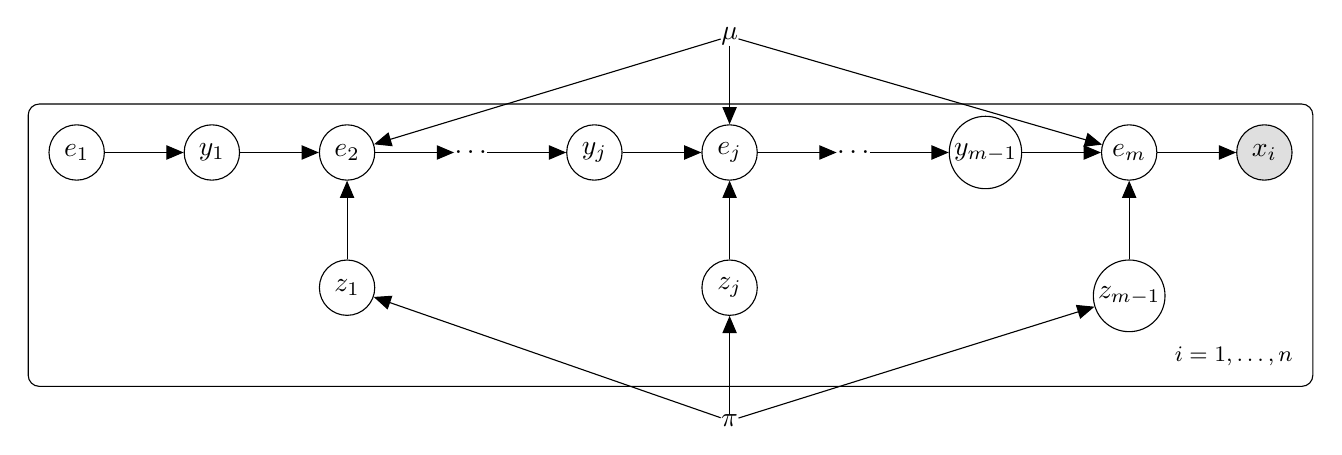
\begin{tikzpicture}
  \node[obs]                               (xi) {$x_i$};
  \node[latent, left=of xi]               (em) {$e_m$};
  \node[latent, below=of em]               (zm1) {$z_{m-1}$};
  \node[latent, left=of em]               (ym1) {$y_{m-1}$};
  \node[const, left=of ym1]               (dots2) {$\ldots$};
  \node[latent, left=of dots2]               (ej) {$e_{j}$};
  \node[latent, below=of ej]               (zj) {$z_{j}$};
  \node[latent, left=of ej]               (yj) {$y_{j}$};
  \node[const, left=of yj]               (dots1) {$\ldots$};
  \node[latent, left=of dots1]               (e2) {$e_2$};
  \node[latent, below=of e2]               (z1) {$z_1$};
  \node[latent, left=of e2]               (y1) {$y_1$};
  \node[latent, left=of y1]               (e1) {$e_1$};
  \node[const, above=of ej]    (mu) {$\mu$};
  \node[const, below=of zj, yshift=-.25cm]  (pi) {$\pi$};

  \edge{e1}{y1};
  \edge{y1}{e2};
  \edge{z1}{e2};
  \edge{e2}{dots1};
  \edge{dots1}{yj};
  \edge{yj}{ej};
  \edge{zj}{ej};
  \edge{ej}{dots2};
  \edge{dots2}{ym1};
  \edge{ym1}{em};
  \edge{zm1}{em};
  \edge{em}{xi};
  \edge {mu} {e2, ej, em};
  \edge {pi} {z1,zj, zm1};

  \plate[inner sep=.25cm] {} {(xi)(e1)(zm1)(z1)} {$i=1, \ldots, n$};
\end{tikzpicture}
\end{adjustbox}
\caption{Graphical model of the stochastic Binary Ordinal Search.}
\label{fig:graphical_model}
\end{figure}

%\ar{Do a figure for the Mixture case}
%\tm{Maybe, although it does not give much more information since it can be trivially derived from this one. Good job for the figure by the way}
%\ar{Agreed, and probably too complicated to do anyways}


\subsection{Parameter estimation}
\paragraph{EM algorithm.} In the univariate case, the underlying BOS distribution of a data sample $(x_1, \ldots, x_n)$ can be estimated using the Expectation-Maximization (EM) algorithm. The main idea behind EM is to iteratively compute the parameters $(\mu, \pi)$ of the distribution to maximize the log-likelihood until convergence when the model is explained by latent variables that are not observed with the data as it is the case with the BOS distribution \citep{biernacki2016model}.
\begin{enumerate}
    \item Initialization: The parameters of the distribution are initialized using a pre-defined heuristic. In our case, we initialize $(\mu^{(0)}, \pi^{(0)})$ randomly in their respective range.
    \item Expectation step: The latent variables $(c_i)_{i \in \{1, \ldots, n\}}$ are estimated using the current approximation of the parameters $(\mu^{(t)}, \pi^{(t)})$. This consists in computing the posterior probability of every latent variable using the conditional probability formula for all $i\in \{1, \ldots, ..., n\}$
    \begin{equation}
        \mathbb{P}(c_i | x_i, \mu^{(t)}, \pi^{(t)}) = \frac{\mathbb{P}(c_i, x_i| \mu^{(t)}, \pi^{(t)})}{\mathbb{P}(x_i| \mu^{(t)}, \pi^{(t)})}
    .\end{equation}
    This can be computed recursively for the different latent variables using their prior distribution (BOS model):
    \begin{equation}
        \mathbb{P}(e_{j+1}| \mu^{(t)}, \pi^{(t)}) = \sum_{e\in \mathcal{P}(\{1, \ldots, m\})} \mathbb{P}(e_{j+1}|e_j=e,  \mu^{(t)}, \pi^{(t)}) \mathbb{P}(e_j=e| \mu^{(t)}, \pi^{(t)})
    .\end{equation}
    The intermediate conditional probability is obtained by conditioning on the different values that can be taken by $y_j$ and $z_j$ when $e_j=e$:
    \begin{align}
    \mathbb{P}(e_{j+1}|e_j=e, \mu^{(t)}, \pi^{(t)}) &= \sum_{y_j \in e} \mathbb{P}(e_{j+1}|e_j=e, y_j, \mu^{(t)}, \pi^{(t)})\mathbb{P}(y_j|e_j=e) \\
    &\begin{aligned}
        = &\sum_{y_j \in e} (\pi^{(t)}\mathbb{P}(e_{j+1}|e_j, y_j, z_j=1, \mu^{(t)}, \pi^{(t)}) \\ 
        & + (1-\pi^{(t)})\mathbb{P}(e_{j+1}|e_j, y_j, z_j=0, \mu^{(t)}, \pi^{(t)}))\mathbb{P}(y_j|e_j=e)
    .\end{aligned}
    \end{align}
    The components of the sum can be more easily computed by distinguishing between the cases where $z_j=0$ and $z_j=1$ with closed-forms expressions from the prior. \\
    Moreover, for $y_j$, the posterior distribution can also be obtained using the following expression where we also condition on $e_j$:
    \begin{equation}
    \mathbb{P}(y_j| \mu^{(t)}, \pi^{(t)}) = \sum_{e\in \mathcal{P}(\{1, \ldots, m\}} \mathbb{P}(y_j|e_j=e, \mu^{(t)}, \pi^{(t)})\mathbb{P}(e_j=e| \mu^{(t)}, \pi^{(t)})
    .\end{equation}
    For $z_j$, $\mathbb{P}(z_j| \mu^{(t)}, \pi^{(t)})$ is a Bernoulli variable of probability $\pi^{(t)}$ so it can easily be expressed:
    \begin{equation}
    \mathbb{P}(z_j| \mu^{(t)}, \pi^{(t)}) = \begin{cases}
        \pi^{(t)}\quad &\text{if } z_j = 1\\
        1 - \pi^{(t)}\quad &\text{if } z_j = 0
        \end{cases}
    .\end{equation}
    %\ar{How does this allow to derive $\mathbb{P}(c_{ij}, x_i| \mu, \pi)?$. Ok}
    Note that since in the BOS model $e_m$ is identified with $x_i$, we get the following joint distribution for all the latent variables $c_i$ with the observation $x_i$: 
    \begin{equation}
       \mathbb{P}(c_i,x_i| \mu^{(t)}, \pi^{(t)}) = \mathbb{P}(e_m|c_i, \mu^{(t)}, \pi^{(t)})\mathbb{P}(c_i| \mu^{(t)}, \pi^{(t)})
    .\end{equation}
    \item Maximization step: During this step, the next iteration of the parameters $(\mu^{(t+1)}, \pi^{(t+1)})$ that maximizes the log-likelihood of observing the data taking into account the latent-variables probabilities computed during the Expectation step. As proposed by \citet{biernacki2016model}, only $\pi$ is updated and $\mu$ is fixed during the entire algorithm. This is done for every possible value of $\mu$ and the value that maximizes the log-likelihood is chosen. \\
    The new value of $\pi$ is given after computing the maximizer of the expectation of the log-likelihood in $\pi$:
    \begin{equation}
    \pi^{(t+1)} = \frac{\sum_{i=1}^N \sum_{j=1}^{m-1} \mathbb{P}(z_{ij}=1|x_i, \mu^{(t)}, \pi^{(t)})}{n(m-1)}
    .\end{equation}
    % \begin{proof}
    % \ar{Add the proof for this formula?}
    % \tm{Yes. I need to check it but not sure there is much to it. Théo opinion ?}
    % \end{proof}
    \footnote{The authors of the paper did not mention how they computed this formula. We computed it by marginalizing on every possible run of the binary search algorithm, leading to high computational cost.

    We use the following expression:
    \begin{align}
        \Pr(z_{ij}=1|x_i, \mu, \pi) &= \sum_{c_i} \Pr(z_{ij}=1, c_i|x_i, \mu, \pi) \\
        &= \sum_{c_i} \Pr(z_{ij}=1|c_i, x_i, \mu, \pi)\Pr(c_i|x_i, \mu, \pi) \\
        &= \sum_{c_i} \Pr(z_{ij}=1|c_i) \frac{\Pr(c_i, x_i|\mu, \pi)}{\Pr(x_i|\mu, \pi)} \\
        &= \frac{1}{\Pr(x_i|\mu, \pi)} \sum_{c_i} \Pr(z_{ij}=1|c_i) \Pr(c_i, x_i|\mu, \pi) 
    \end{align}
    And then:
    \begin{align}
        \sum_{j=1}^{m-1} \Pr(z_{ij}=1|x_i, \mu, \pi) &= \sum_{j=1}^{m-1} \frac{1}{\Pr(x_i|\mu, \pi)}  \sum_{c_i} \Pr(z_{ij}=1|c_i) \Pr(c_i, x_i|\mu, \pi) \\
        &= \frac{1}{\Pr(x_i|\mu, \pi)} \sum_{c_i} \Pr(c_i, x_i|\mu, \pi)  \sum_{j=1}^{m-1} \Pr(z_{ij}=1|c_i)
    \end{align}
    }

\end{enumerate}

\paragraph{AECM algorithm.} Similarly to the EM algorithm, Alternating Expectation-Conditional Maximization (AECM) \citep{meng1997algorithm} is separated in two steps. However, in this case, we consider multivariate ordinal data with different possible distributions (clusters) priors for the data. This is done, just like for the Gaussian Mixture Model case, using latent variables $w_{ik}$ which describe whether the data $x_i$ belongs to the cluster $k$ or not, and parameters $(\alpha_k)_{k\in \{1, \ldots, p\}}$ which describe the probability of belonging to each cluster. 
\begin{enumerate}
    \item Expectation step: In this case, the expectation step consists in just computing the probability for every data point to belong to each cluster:
    \begin{equation}
        \mathbb{P}(w_{ik}=1|x_i, \alpha^{(t)}, \mu^{(t)}, \pi^{(t)}) = \frac{\alpha_k^{(t)}\mathbb{P}(x_i|w_{ik}=1, \mu_k^{(t)}, \pi_k^{(t)})}{\sum_{l=1}^p\alpha_l^{(t)}\mathbb{P}(x_i|w_{il}=1, \mu_l^{(t)}, \pi_l^{(t)})}.
    \end{equation}
    \item Maximization step: The parameters are updated using the new expected values for belonging to the different cluster. Since there are two groups of latent variables, the clusters variables $\alpha_k^{(t)}$ are updated first to maximize the log-likelihood:
    \begin{equation}
    \alpha_k^{(t+1)} = \frac{1}{n} \sum_{i=1}^n \mathbb{P}(w_{ik}=1|x_i, \alpha^{(t)}, \mu^{(t)}, \pi^{(t)}).
    \end{equation}
    And then the parameters $(\mu_k^{(t+1)}, \pi_k^{(t+1)})$ are updated after using an EM algorithm in the univariate case for every cluster $k$ and for every dimension of the multivariate variables independently using the data on the corresponding dimension.
\end{enumerate}


\section{Method}

We suppose that we aim to cluster multivariate data. Each dimension has data generated by a random process parametrized by parameters that are dependant of the cluster. To estimate the cluster it is possible to use the AECM algorithm introduced in~\citep{meng1997algorithm}. This algorithm is quite generic and only requires to be able to estimate the univariate parameters of a weighted set of data points. We present this algorithm in section~\ref{sec:aecm}.

Similarly to~\cite{biernacki2016model} we focus on ordinal data. Therefore we suppose that each dimension follow a process that generates ordinal categories. 
In section~\ref{sec:univariate}, we present two random processes to model ordinal data the binary ordinal search (BOS) model from~\cite{biernacki2016model} and the globally ordered data (GOD) model.

To apply the proposed methods the each dimension of the data should represent an ordinal categorie. These categories must respect the following properties:

\begin{itemize}
\item The categories must be well-ordered (ordinal data): The categories are linearly ordered, and each non-empty subset contains the least element. This implies that any element can be compared to any other, and we can enumerate all the categories in increasing order.

\item The set of categories is finite. This simplifies the previous assumption to the existence of a linear ordering. This assumption is necessary to ensure that the stochastic search terminates after a fixed number of steps, implying a finite number of possible runs of the search.
\end{itemize}





\subsection{AECM algorithm.} 
\label{sec:aecm}

\tm{Introduce all the requrired notation in a clear manner (maybe in the previous section), so it is easy to find the signification of each letter}
Similarly to the EM algorithm, Alternating Expectation-Conditional Maximization (AECM) \citep{meng1997algorithm} is separated in two steps. However, in this case, we consider multivariate ordinal data with different possible distributions (clusters) priors for the data. Similar to the Gaussian Mixture Model case, the algorithm use latent variables $w_{ik}$ which describe whether the data $x_i$ belongs to the cluster $k$ or not, and parameters $(\alpha_k)_{k\in \{1, \ldots, p\}}$ which describe the probability of belonging to each of the $p$ cluster. We also note $\theta_k^{(t)}$ the parameters of the $k$-th cluster at the $t$-th iteration.
\begin{enumerate}
    \item Expectation step: The expectation step consists in computing the probability for every data point to belong to each cluster:
    \begin{equation}
        \mathbb{P}(w_{ik}=1|x_i, \alpha^{(t)}, \theta^{(t)}) = \frac{\alpha_k^{(t)}\mathbb{P}(x_i|w_{ik}=1, \theta_k^{(t)})}{\sum_{l=1}^p\alpha_l^{(t)}\mathbb{P}(x_i|w_{il}=1, \theta_l^{(t)})}.
    \end{equation}
    \item Maximization step: The parameters are updated using the new expected values for belonging to each cluster. Since there are two groups of latent parameters, the clusters weights $\alpha_k^{(t)}$ are updated first to maximize the log-likelihood:
    \begin{equation}
    \alpha_k^{(t+1)} = \frac{1}{n} \sum_{i=1}^n \mathbb{P}(w_{ik}=1|x_i, \alpha^{(t)}, \theta^{(t)}).
    \end{equation}
    And then the parameters $(\theta_k^{(t + 1)})$ are updated after using the internal parameters estimation for each cluster unsing the observations weighted by the probability of belonging to the cluster.

\tm {Modify algorithm below to be more specific (use the model of ternary search algorithm)}
\begin{algorithm}
\caption{AECM}
\label{alg:aecm}
\begin{algorithmic}[1]
\Require Number of clusters $K$
\While {log-likelihood increase}
    \State \textbf{E Step}: For each sample, compute the conditional probability of belonging to each cluster given the current estimation of the model parameters, ie.
    $$\text{For $i\in\{1,...,n\}$ and $k\in\{1,...,K\}$, compute }p(i\in C_k | x_i, \boldsymbol{\alpha}, \boldsymbol{\mu}, \boldsymbol{\pi})$$
    \State \textbf{M Step}: Update the estimation of the model parameters using the probabilities of the previous step.
    \State \quad - Mixing proportion $\boldsymbol{\alpha}$
    \State \quad - Component parameters $(\mu_k,\pi_k)_{i=k}^K$ using the parameter estimation algorithm of the BOS or GOD models
\EndWhile
\end{algorithmic}
\end{algorithm}
\end{enumerate}



\subsection{Univariate model}
\label{sec:univariate}

We now wan't a random process to model univariate ordinal data among a finite numbers of categories.
As we suppose that we only care for the order of the categories we can can without loss of generality consider our categories as $[[1, m]]$ (when there is $m$ categories). Therefore if we have $\theta$ the parameters of our model, a model is gives $\forall i \in [[1, m]], P(X = i | \theta)$ if $X$ was generated from our random process. 

As we should represent data have having a common source we can suppose that there is an underlying true category $\mu \in [[1, m]]$ and put it as a parameter. In addition it is natural to add a precision parameter $\pi$. This is the case for the BOS model and the GOD model. 

In the following sections we present how to estimate those parameters for a generic law, then we present the BOS model and how to apply this estimation technique then we do the same with the GOD model.


\subsubsection{Notations and goal}

Let suppose that we have a set of $n$ independant observations $X = (x_i)_{i \in [n]}$, wehre $x_i \in [[1, m]]$ follow a distribution $P$ with parameters $\mu, \pi$ with $\mu \in [[1, m]]$ and $\pi \in [[a, b]]$. We want to estimate $\mu$ and $\pi$. We choose the estimate that maximize the likelihood of the data.
$$(\mu, \pi) = \argmax_{(\mu, \pi) \in [[1, m]] \times [[a, b]]} P(X | \mu, \pi)$$

As the data are independant, we have:
$$P(X | \mu, \pi) = \prod_{i=1}^n P(x_i | \mu, \pi)$$

As the number of possible values for $x$ is finite, we can group the data by values and count the number of occurences of each value. Let $n_i$ be the number of occurences of $i$ in the data. We have:
$$P(X | \mu, \pi) = \prod_{i=1}^m P(i | \mu, \pi)^{n_i}$$

In the AECM algorithm, each data point has a weight $w_i$. As previously, we can suppose without loss of generality that we have only one observation of each value with a specific weight (we can always group the data by values and sum the weights of the observations). With the weights $W \in \mathbb{R}_+^n$ where $w_i$ is the weight of the value $i$, we can write the weighted likelihood as:

$$P(W | \mu, \pi) = \prod_{i=1}^m P(i | \mu, \pi)^{w_i}$$

We can also write the weighted $\log$-likelihood as:

$$L_W(\mu, \pi) := \log P(W | \mu, \pi) = \sum_{i=1}^m w_i \log P(i | \mu, \pi)$$


\subsubsection{Optimization}
\label{sec:univariate_generic_estimation}

To estimate $\mu$ and $\pi$, the idea proposed for the BOS-model in REF is to use the Expectaion-Maximization algorithm. However they note that it is easier to first estimate $\pi$ for every possible value of $\mu$ and then to estimate $\mu$ using the estimated $\pi$. In forulas, we have:


$$\hat{\pi_{\mu}} = \argmax_{\pi \in [[a, b]]} P(W | \mu, \pi)$$
$$\hat{\mu} = \argmax_{\mu \in [[1, m]]} \max_{\pi \in [[a, b]]} P(W | \mu, \pi) = \argmax_{\mu \in [[1, m]]} P(W | \mu, \hat{\pi_{\mu}})$$

Once we have the estimates $\hat{\pi_{\mu}}$ for every possible value of $\mu$, it is easy to estimate $\mu$ by choosing the value of $\mu$ that maximize the weighted likelihood as it requires only to compute the likelihood for every possible value of $\mu$ and to choose the maximum.

Estimating $\pi$ for a given $\mu$ is a one-dimensional optimization problem. We can use the EM algorithm to solve it but it may be possible to use a direct optimization algorithm. For example if the function $\pi \mapsto L_W(\mu, \pi)$ is stricly concave (or constant), we can the ternary search algorithm (or trisection algorithm) to find the maximum.

\paragraph{Concavity of the weighted likelihood}

Suppose we have:

$$\forall x \in [[1, m]], \pi \mapsto P(x | \mu, \pi) \text{ is strcictly $\log$-concave}$$

Then we have, $\pi \mapsto L_W(\mu, \pi)$ is stricly concave as positive linear combination of concave functions are concave.

\paragraph{Ternary search algorithm}

\todo{TODO} 
%(see https://en.wikipedia.org/wiki/Ternary_search)

\paragraph{Evaluating the likelihood}

To run the ternary search algorithm, we need to be able to evaluate the log-likelihood for a given value of $\pi$ efficiently.
The log-likelihood is the sum of $m$ log of the likelihoods of individual values.
Hence the complexity will be $\Theta(m C_E(m))$ where $C_E(m)$ is the complexity of computing the likelihood for a single value of $x$.

In the case of the BOS model, we can notice that $\forall x \in [[1, m]], \pi \mapsto P(x | \mu, \pi)$ is polynomial of degree $\Theta(m)$ with coefficients that depend on $m$, $i$ and $\mu$. This is alsmost alos the case for the GOD mdoel in the sense that the following reasonning holds. As the function is polynomial, we can precompute these coefficients and then evaluate the likelihood of one value in $\Theta(m)$ operations. This gives a complexity of $\Theta(m^2)$ to evaluate the total likelihood of $W$ for a given $\mu$ and $\pi$. 

An important point is we excluded the cost of the precomputations of the coefficients. This cost is not necessary negligible but countrary to the evaluation of the likelihood, it is only done once for one $m$ and can be then used for all iterations of the AECM algorithm and the ternary search algorithm.


\paragraph{Complexity}

We note $n$ the numbre of observations, $m$ the number of possible values for $x$ and $\epsilon > 0$ the precision of the estimate of $\pi$.

We can first group the data by values and sum the weights of the observations. This can be done in $\Theta(n)$ operations.

Then to estimate $\pi$ for a given $\mu$, we can use the ternary search algorithm. The number of iterations of the algorithm is $\Theta(\log \frac{b - a}{\epsilon})$. For each iteration, we need to compute the likelihood for two values of $\pi$. If we note $C_E(m)$ the complexity of computing the likelihood for a given value of $\pi$, we have a complexity of $\Theta(\log \frac{b - a}{\epsilon} C_E(m))$.

Finally, to estimate $\mu$, we need to compute the likelihood for every possible value of $\mu$. This gives a total complexity of $\Theta(m C_E(m) \log \frac{b - a}{\epsilon} )$.

In our case we have $C_E(m) = \Theta(m^2)$ and $[a, b] \subset [0, 1]$ which gives a complexity of $\Theta(m^3 \log \frac{1}{\epsilon})$ (without taking into account the precomputations of the coefficients).



\subsection{Stochastic Binary Ordinal Search} 

The BOS model is inspired by a standard binary search with added noise in the comparison. Consequently, the algorithm may at times misidentify the next subset for the search, ultimately causing it to overlook the sought-after value.


\subsubsection{Probabilistic model}

The stochastic binary ordinal search unfolds as follows: Let $m$ be the number of categories. Then, for at most $m-1$ steps, we perform the following three operations.
We start with the full set of categories, denoted as $e_1 = \bbrack{1,m}$. Then we perform the following steps:

At step $j$, we start with a subset of all the categories, denoted as $e_j = \bbrack{l_j, u_j - 1} \subseteq \bbrack{1,m}$.

\begin{enumerate}
    \item Sample a breakpoint $y_j$ uniformly in $e_j$ ($y_j \sim \mathcal{U}(e_j)$).
    \item Draw an accuracy indicator $z_j$ from a Bernoulli distribution with parameter $\pi$ ($z_j \sim \text{Bernoulli}(\pi)$).
    A value of $z_j=1$ indicates that the comparison is perfect, and the next step will be computed optimally. A value of $z_j=0$ implies a blind comparison at the next step.
    \item Determine the new subset $e_{j+1}$ for the next iteration. Firstly, split the subset into three intervals, namely $e_j^- = \bbrack{l_j, y_j - 1}$, $e_j^= = \set{y_j}$, and $e_j^+ = \bbrack{y_j + 1, u_j - 1}$. $e_{j+1}$ will be chosen among these intervals. If the comparison is blind ($z_j=0$), randomly select the interval with a probability proportional to its size. Alternatively, if $z_j=1$ and the comparison is perfect, select the interval containing $\mu$ (or, by default, the one closest to it).
\end{enumerate}
After $m-1$ steps, the resulting interval contains a single value, which is the observed result $e_m=\set{x}$ of the BOS model.


\begin{figure}[htbp]
\centering
\begin{adjustbox}{width=\textwidth}
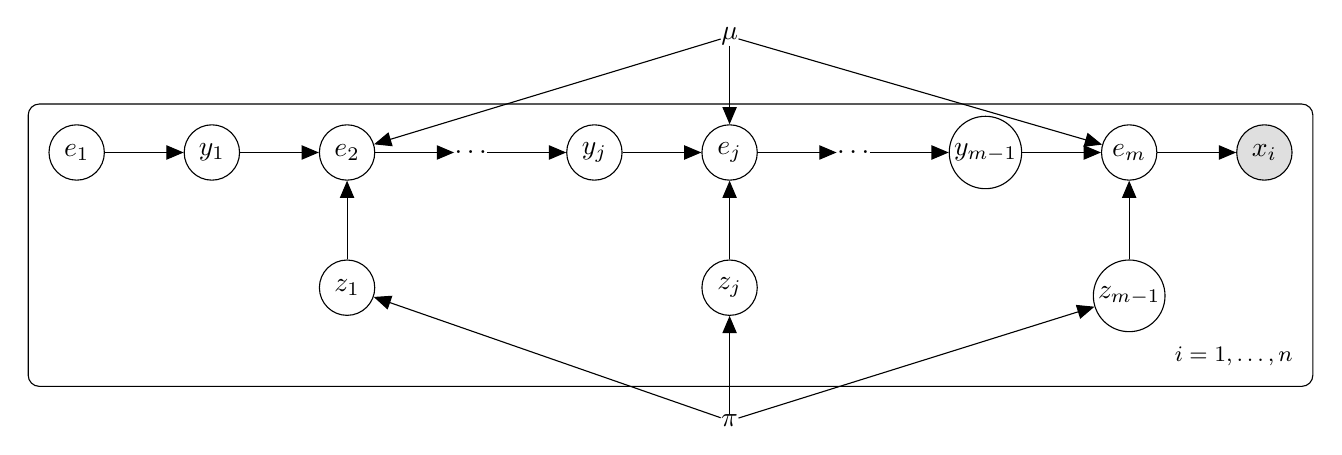
\begin{tikzpicture}
  \node[obs]                               (xi) {$x_i$};
  \node[latent, left=of xi]               (em) {$e_m$};
  \node[latent, below=of em]               (zm1) {$z_{m-1}$};
  \node[latent, left=of em]               (ym1) {$y_{m-1}$};
  \node[const, left=of ym1]               (dots2) {$\ldots$};
  \node[latent, left=of dots2]               (ej) {$e_{j}$};
  \node[latent, below=of ej]               (zj) {$z_{j}$};
  \node[latent, left=of ej]               (yj) {$y_{j}$};
  \node[const, left=of yj]               (dots1) {$\ldots$};
  \node[latent, left=of dots1]               (e2) {$e_2$};
  \node[latent, below=of e2]               (z1) {$z_1$};
  \node[latent, left=of e2]               (y1) {$y_1$};
  \node[latent, left=of y1]               (e1) {$e_1$};
  \node[const, above=of ej]    (mu) {$\mu$};
  \node[const, below=of zj, yshift=-.25cm]  (pi) {$\pi$};

  \edge{e1}{y1};
  \edge{y1}{e2};
  \edge{z1}{e2};
  \edge{e2}{dots1};
  \edge{dots1}{yj};
  \edge{yj}{ej};
  \edge{zj}{ej};
  \edge{ej}{dots2};
  \edge{dots2}{ym1};
  \edge{ym1}{em};
  \edge{zm1}{em};
  \edge{em}{xi};
  \edge {mu} {e2, ej, em};
  \edge {pi} {z1,zj, zm1};

  \plate[inner sep=.25cm] {} {(xi)(e1)(zm1)(z1)} {$i=1, \ldots, n$};
\end{tikzpicture}
\end{adjustbox}
\caption{Graphical model of the stochastic Binary Ordinal Search.}
\label{fig:graphical_model}
\end{figure}

%\ar{Do a figure for the Mixture case}
%\tm{Maybe, although it does not give much more information since it can be trivially derived from this one. Good job for the figure by the way}
%\ar{Agreed, and probably too complicated to do anyways}




\subsubsection{Parameter estimation}

We want to estimate $\pi$ and $\mu$ from a sample $(1, \dots, m)$ with weights $W \in \RR_{+}^m$ generated by the GOD model. We aim at maximizing the likelihood of the sample : $\Pr(W | \pi, \mu)$. We proceed as explained in section~\ref{sec:univariate_generic_estimation}. All the proofs of this section are detailed in appendix~\ref{appendix:bos_proofs}, we only give here the main results.

\paragraph{Likelihood evaluation}

\begin{thm}[Likelihood is polynomial]
    $\forall m \in \NN^*, \forall x \in \bbrack{1, m}, \forall \mu \in \bbrack{1, m}$,:
    \[ \pi \mapsto \Pr(x | \mu, \pi) \]
    is a polynomial function of degree at most $m - 1$.  
\end{thm}

\begin{definition}
    We denote by $u[\mu, x, d]$ the coefficient of the polynomial of degree $d$ in the polynomial expansion of $\pi \mapsto \Pr(x | \mu, \pi)$ \textit{ie}:
    \[ \Pr(x | \mu, \pi) = \sum_{d = 0}^{m - 1} u[\mu, x, d] \pi^d \]
\end{definition}

We show that the likelihood of a single observation is a polynomial function of degree at most $m - 1$ in $\pi$. This result is important because, once the coefficients are known, it implies that the likelihood of a single observation can be computed in $\Theta(m)$ and the $\log$-likelihood of a sample (which has at most $m$ distinct values) in $\Theta(m^2)$ operations. 
For a fixed $m$, there is only $m^2$ polynomials to compute and store (one for each couple $(x, \mu)$), which leads to $m^3$ coefficients to store. We will show in the next paragraph~\ref{sec:bos_coefficients} that these coefficients can be computed in $\mathcal O(m^5)$ operations.

\paragraph{Computing the coefficients}
\label{sec:bos_coefficients}

\begin{definition}
    To simplify the comprehension of the following results, we introduce a notation for the probability in the case of $h$ categories~\footnote{This notation may seem different from the one used in the appendix but it is equivalent.}:
    \[ \bosl{x}{\mu}{h} := \Pr(x + 1 | \mu + 1, \pi) \text{ with }h\text{ categories}\]
\end{definition}

\begin{thm}[Computing the likelihood]
    \label{thm:computing_likelihood_bos}
    $\forall m \in \NN^*, \forall x \in \bbrack{1, m}, \forall \mu \in \bbrack{1, m}, \forall \pi \in [0, 1]$:

\begin{equation}
    \begin{aligned}
        \bosl{x}{\mu}{h}
        &=\frac{1}{h} \sum_{y = x + 1}^{h - 1} \bosl{x}{\mu}{y} \left[ \left( \indickronecker{\mu < y} - \frac{y}{h} \right) \pi + \frac{y}{h} \right] \\
            &+\frac{1}{h} \ \qquad \left[ \left( \indickronecker{\mu = x \lor (x = 0 \land \mu \leq x) \lor (x = h - 1 \land \mu \geq x)} - 1 \right) \pi +  \frac{1}{h} \right] \\
            &+\frac{1}{h} \sum_{y = 0}^{x - 1}\bosl{x - y}{\max(0, \mu - y)}{h - y}    \left[ \left( \indickronecker{\mu > y} - \frac{h - y - 1}{h} \right) \pi + \frac{h - y - 1}{h} \right]
    \end{aligned} \\
\end{equation}
\end{thm}

This theorem gives a recursive formula to compute the likelihood of a single observation. Using this formula, we can construct a dynamic programming algorithm to compute the coefficients of the polynomials. To do this we proceed by increasing $x$, $\mu$ and $h$. We do directly the multiplication of the polynomials.

Each term of the sum require the multiplication of a polynomial of degree at most $m - 1$ by a polynomial of degree $2$ which gives a cost of $O(m)$. The sum has at most $m$ terms, which gives a cost of $O(m^2)$. We need to apply this formula for each $(x, \mu, h)$ which gives a cost of $O(m^5)$.

\paragraph{Log concavity}

\begin{thm}[Log concavity of the BOS model]
    $\forall m \in \NN^*, \forall x \in \bbrack{1, m}, \forall \mu \in \bbrack{1, m}$:
    \[\pi \mapsto \Pr(x | x, \mu, \pi) \] 
    is $\log$-concave on $[0, 1]$.
\end{thm}

As explained in section~\ref{sec:univariate_generic_estimation}, we directly have that $\forall \mu \in \bbrack{1, m}, \pi \mapsto L_W(\pi, \mu)$ is concave. Hence we can use a ternary search algorithm to estimate $\pi$ for a given $\mu$.

\paragraph{title}

As presented in section~\ref{sec:univariate_generic_estimation}, we can estimate $\mu, \pi$ in $\mathcal O(m^3 \log \frac{1}{\epsilon})$ operations once the coefficients $u$ are computed. The coefficients $u$ can be computed in $\mathcal O(m^5)$ operations and stored in $\mathcal O(m^3)$ space. This is a major improvement compared to the EM algorithm proposed in~\cite{biernacki2016model}. Indeed we give a fully polynomial time algorithm with precision guarantees, while the EM algorithm has no guarantees on the precision and the proposed algorithm is exponential in the number of categories.

\tr{TODO: add a the run time comparisons}





\subsection{Alternative model "Globally Ordered Data" (GOD)}


% \tm {Laisser présentation du modèle, graphical model, estimation des paramètres. Tous les lemmes et théorèmes vont en annexe.}

In the article under study, the authors motivated the use of binary search with the following sentence: "In order to minimize the number of potentially wrong comparisons, it
is necessary to minimize the number of comparisons performed during the search process.". However, we believe that minimizing the number of incorrect comparisons may not be an adequate intuition, and it is more crucial to minimize the probability of making a wrong guess. Motivated by this perspective, we have developed an alternative model where the data is compared with each category with some noise. We will refer to this model as the Globally Ordered Data (GOD) model.

We still consider a search for the parameter $\mu$ among the ordered categories. However, instead of conducting a binary search, we compare each category to the parameter $\mu$ and with probability $\pi$ we get the correct answer. After making all these comparisons, we then select the category that corresponds to the minimum number of comparison error. This approach display similar properties to the BOS model such as a unique mode, probability distribution decrease on either side of the mode, and the flexibility to accommodate uniform or Dirac distribution.

\subsubsection{Probabilistic model}

\begin{figure}[htbp]
    \centering
    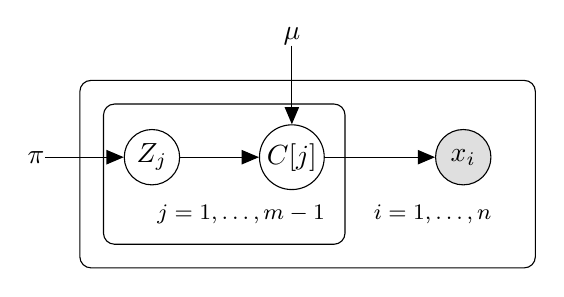
\begin{tikzpicture}
     \node[obs]                               (xj) {$x_i$};
     \node[latent, left=1.4cm of xj]               (cj) {$C[j]$};
     \node[latent, left=of cj]               (zj) {$Z_j$};
     \node[const, left=of zj]    (pi) {$\pi$};
     \node[const, above=of cj]  (mu) {$\mu$};
    
     \edge{zj}{cj};
     \edge{cj}{xj};
     \edge {mu} {cj};
     \edge {pi} {zj};
    
     \plate[inner sep=.55cm] {}{(xj)(cj)(zj)}{$i=1, \ldots, n$};
     \plate[inner sep=.25cm] {}{(cj)(zj)}{$j=1, \ldots, m - 1$};
    \end{tikzpicture}
    \caption{Graphical model of the GOD model.}
    \label{fig:god_graphical_model}
\end{figure}
    
The GOD model for $m$ categories is characterized by two parameters $\mu \in \bbrack{1, m}, \pi \in ]\frac{1}{2}, 1]$. The observed data is only the selected category $x$. The latent variables are the vector $Z = (Z_1,...,Z_{m-1}) \in \set{0, 1}^{m - 1}$ and $C \in \set{0, 1}^{m-1}$.
$(Z_j)_{j\in\bbrack{1,m-1}}$ is a vector of independent Bernoulli variables, with parameter $\pi$. For $j \in \bbrack{1, m-1}$, $Z_j$ indicates whether the comparison with the category $j$ is correct $(Z_j=1)$ or not $(Z_j=0)$. $C$ is the vector containing the $m$ results of the comparisons depending on both $Z$ and the parameter $\mu$. It is defined as follows:
\[
\forall j \in \bbrack{1, m-1}, C[j] = \begin{cases}
    (\mu < j) & \text{if}\  Z_j = 1\\
    (\mu \not< j) & \text{if}\  Z_j = 0
\end{cases} \]

The GOD model will generate $x \in \bbrack{1, m}$ such that $x \sim \mathcal{U}(\argmin_{k \in \bbrack{1, m}} \norm{c - E_k}_1)$. We can interpret this as a probability maximization as stated in Theorem~\ref{thm:projection}. The graphical model associated with this probabilistic model is depicted on Figure \ref{fig:god_graphical_model}.


\begin{definition}[Heaviside vector]
    For $k \in \bbrack{1, m}$, we define:
    \[E_k := (1)^{k-1} (0)^{m - k} = (\underset{k-1}{\underbrace{1, \dots, 1}}, \underset{m - k}{\underbrace{0, \dots, 0}} ). \]
\end{definition}


\begin{thm}
    \label{thm:projection}
    If we suppose that the prior distribution of $\mu$ is uniform over $\bbrack{1, m}$ and $\pi > \frac{1}{2}$, then \(\forall c \in \set{0, 1}^{m-1}\),
    \[\argmax_{k \in \bbrack{1, m}} \Pr(\mu = k | C = c) = \argmin_{k \in \bbrack{1, m}} \norm{c - E_k}_1.\]
\end{thm}

The proof can be found in appendix~\ref{thm:projection_appendix}.

\subsubsection{Parameter estimation}

We want to estimate $\pi$ and $\mu$ from a sample $X = (x^1, \dots, x^n) \in \bbrack{1, m}^n$ of $n$ observations of $x$ generated by the GOD model. We aim at maximizing the likelihood of the sample : $\Pr(X | \pi, \mu)$. 

We define for $x \in \bbrack{1, m}$, 
\[ \mathcal{C}_x := \set{c \in \set{0, 1}^{m-1} | x \in \argmin_{k \in \bbrack{1, m}} \norm{c - E_k}_1 } .\]

\begin{lemma}
    \label{lemma:p_x_c_knowing_pi_mu}
    \[\Pr(x, c | \pi, \mu) = \indic{}_{\mathcal{C}_x}(c) \frac{\pi^{m - 1 - \norm{c - E_{\mu}}_1} (1 - \pi)^{\norm{c - E_{\mu}}_1}}{\card{\argmin_{k \in \bbrack{1, m}} \norm{c - E_k}_1}} .\]
\end{lemma}

Proof in appendix~\ref{lemma:p_x_c_knowing_pi_mu_appendix}.


\begin{definition}
    We define for $x \in \bbrack{1, m}, \mu \in \bbrack{1, m}, d \in \bbrack{0, m-1}$:
    \[ u(\mu, x, d) := \sum_{c \in \mathcal{C}_x / \norm{c - E_{\mu}}_1 = d}  \card{\argmin_{k \in \bbrack{1, m}} \norm{c - E_k}_1}^{-1} .\]
\end{definition}

For a given $m$, $u$ can be fully computed in $\mathcal O(m^2 2^m)$ time. We believe that it might be possible to compute it in polynomial time, but we did not have time to find how. Although still costly, it only needs to be computed once for a given $m$ and can be stored in $\mathcal O(m^3)$ space.
% copilot :
% Indeed, for a given $x$ and $\mu$, we have $\card{\mathcal{C}_x} = \binom{m}{\mu}$ and $\card% {\argmin_{k \in \bbrack{1, m}} \norm{c - E_k}_1} = \binom{m}{\mu - d} \binom{m - \mu + d}{d}$. Therefore, we have:

\begin{definition}[weighted likelihood]
    For the AECM algorithm, we define the weighted likelihood with weights $w \in \RR_+^n$:
    \[ \Pr((X, W') | \pi, \mu) = \prod_{i=1}^{n} \Pr(x^i | \pi, \mu)^{w'_i} \]

    As  $X \in \bbrack{1, m}^n$, without loss of generality, we can assume that we have exactly $m$ weights: $W = (\sum_{i / x^i = 1} W'[i], \dots, \sum_{i / x^i = m} W'[i])$. Hence with $W \in \RR_+^m$:
    \[ \Pr((X, W') | \pi, \mu) = \Pr(W | \pi, \mu) = \prod_{i=1}^{m} \Pr(i | \pi, \mu)^{w_i} \]

    And again, without loss of generality, we can assume that every sample is weighted with weight $w'_i = 1$.

    Hence we now consider data as a vector $W \in \RR_+^m$.
\end{definition}

\begin{thm}[Data likelihood]
    \label{thm:p_xs_knowing_pi_mu}
    \begin{align}
        \Pr(W | \pi, \mu) 
        &= \pi^{(m-1)\sum_{i=1}^{m} w_i} \prod_{i=1}^{m} \left[\sum_{d = 0}^{m-1} \left(\frac{1 - \pi}{\pi}\right)^d u(x^i, \mu, d) \right]^{w_i}\\
        L_W(\pi, \mu) 
        &= (m-1)\left(\sum_{i=1}^{m} w_i\right) \log\pi + \sum_{i=1}^{m} w_i \log\left[ \sum_{d = 0}^{m-1} \left(\frac{1 - \pi}{\pi}\right)^d u(x^i, \mu, d) \right]
    \end{align}
\end{thm}
\begin{proof}
    We just use the fact that the random variables $(x^i)_{i=1}^n$ are independent and Theorem~\ref{thm:p_x_knowing_pi_mu} from Appendix~\ref{appendix:god}.
\end{proof}

Similarly to the BOS model, we estimate $\hat{\pi}$ for each fixed $\mu$. Then we keep the couple $(\hat{\pi}, \mu)$ that maximizes the log-likelihood.
To estimate $\pi$ for a fixed $\mu$, we considered different possibilities. The first option is to use a simple grid search. This is feasible as evaluating $L_X$ is not too costly and can be done in $\mathcal O(nm)$ time. Then, we considered using the EM algorithm, similar to the approach taken for the BOS model. We derived the update rules and implemented it. Unfortunately, there was an issue with our EM implementation for this model that we did not succeed in fixing.

\begin{figure}
    \centering
    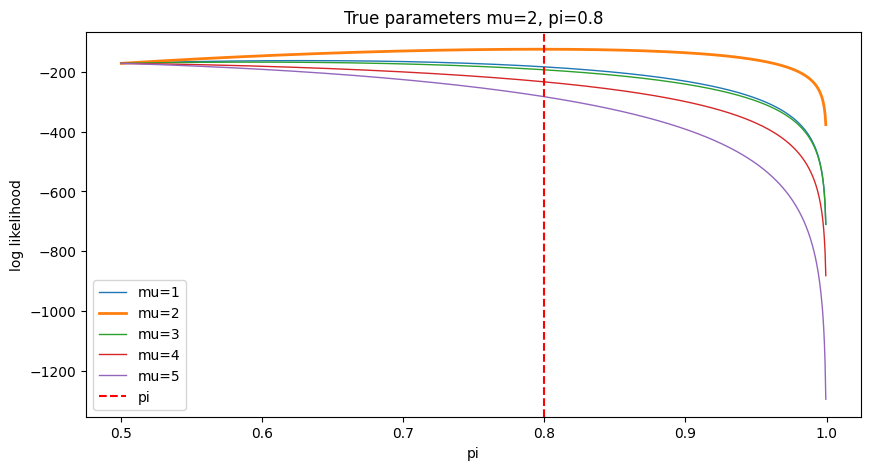
\includegraphics[width=0.5\textwidth]{Attachments/log_likelihoods.png}
    \caption{Log-likelihoods for each possible $\mu$ for $n = 100$ samples with the true parameters being $m = 5$, $\mu=2$ and $\pi = 0.8$ }
    \label{fig:log_likelihoods}
\end{figure}

We can examine the log-likelihood functions in Figure~\ref{fig:log_likelihoods} to understand how to optimize them. As observed, each of the functions $\pi \mapsto L_X(\pi, \mu)$ is concave on the interval $[0.5, 1]$.

\begin{thm}
    \label{thm:log_likelihood_concave}
    $\forall \mu \in \bbrack{1, m}$, 
    \[ \pi \mapsto L_W(\pi, \mu) \]
    is concave on $[0.5, 1]$.
\end{thm}

For the proof, see appendix~\ref{thm:log_likelihood_concave_appendix}.

As the log-likelihood is concave, we can employ the trichotomy method to find the maximum with a few evaluations of $L_W$. For a precision $\epsilon$, the trichotomy method requires $k \geq \frac{\lg_2 \epsilon + 1}{1 - \lg_2 3} = \mathcal O(\ln \epsilon)$ steps and therefore $\mathcal O(\ln \epsilon)$ evaluation of $L_X$.

\paragraph{Complexity}

The pre-computational cost of computing $u$ is $\mathcal O(m^2 2^m)$.

The evaluation of $L_W$ is done in $\mathcal O(n + m^2)$. We run the trichotomy algorithm $m$ times, and therefore, we evaluate $L_W$ $\mathcal O(m \ln \epsilon)$ times. The total cost is thus $\mathcal O(n + m^2 \ln \epsilon)$ for $m$ being the number of categories, $n$ the number of observations and $\epsilon$ being the precision on $\pi$.

%EM on the probabilistic model + algorithm
\section{Experiments}
In this section, we try to evaluate the performance of the two models on different datasets. We first present the experimental setup and the datasets used for the experiments. We then present the results obtained for the estimation algorithms on synthetic data and on real-life datasets. We finally try to discuss the results obtained and the relevance of the models. 

The goal of these experiments is to compare the two models but also to individually test their ability to cluster ordinal datasets and to check whether they are able to generalize to real-life datasets.

All of the experiments and table are reproducible using the provided code and datasets using the fixed seeds.

\subsection{Synthetic data}
\paragraph{Experimental setup.}
In this section, we propose to test the AECM algorithm for the BOS and the GOD model on synthetic data in order to check the ability of our proposed estimation methods to correctly estimate the parameters of the dataand to cluster the datasets. 

\paragraph{Evaluating the estimation error.}
We generate data from the BOS and the GOD model with different parameters and with both a random initialization of the parameters and an initialization of the parameters using the K-Means algorithm and then run the AECM algorithm on the generated data to estimate the parameters. We then compare the estimated parameters with the true parameters using the $L_1$ distance between the two vectors similarly to \cite{biernacki2016model}. We repeat this process multiple times for different parameters and average the results to obtain the metrics presented in Table~\ref{tab:results_bos} and Table~\ref{tab:results_god} in Appendix \ref{appendix:metrics_synth}. Runtimes are also measured on the same machine for all the algorithms to evaluate their efficiency.
 \\ \\
\ar{add discusssion on the results}

\paragraph{Clustering performance.}
We also generate data with multiple clusters from different distributions and then run the AECM algorithm on the generated data to estimate the clusters. The goal of this experiment is to check the ability of the models to correctly cluster the data and to check whether the models are able to generalize to different distributions.
The distributions used are the BOS model, the GOD model and discretized blobs.
The following clustering algorithms are used for comparison: K-Means, Gaussian Mixture Models and the BOS and GOD models. The ARI score (section~\ref{sec:evaluation_method}) is used to measure the clustering performance. The results are presented in Table~\ref{tab:ari_synthetic} in Appendix \ref{appendix:metrics_synth}. \\ \\
\ar{Need to add ordinal clustering algorithms that are different?}
\ar{Discussion}

\paragraph{Visualizing the clusters.}
In order to get a better idea of the differences between the clustering methods, t-SNE visualizations \citep{van2008visualizing} are plotted for different disitributions and clustering methods. The visualizations project the categorical datapoints in a continuous space and allow to check whether the estimated clusters are coherent with the true clusters. Since categorical data is used, it is more difficult to separate the clusters with smaller dimensionnal data and when the number of categories is small. Multiple datasets are generated with different parameters in order to highlight these differences. Moreover, as seen in the previous paragraph, it is also easier to cluster the data when the number of categories or features are high.
The results are presented in Figure~\ref{fig:tsne_synthetic} in Appendix \ref{appendix:metrics_synth}. \\ \\
\ar{Discussion}

\paragraph{Parameters of the experiment}

\subsection{Real-life datasets}
\subsubsection{Datasets} One of the main goal of the experiments is to test the ability of the models to generalize to real-life datasets. We therefore propose to test the illustrated methods on real world datasets to check the usefulness of the models on different real-life situations. Since the algorithm is specifically designed for ordinal observations, the datasets need to be adapted for the task. One way to apply to obtain real-life datasets is to quantize continuous datasets of observations that can be categorized (e.g. movies, store products, species...) \citep{skubacz2000quantization}. Another interesting approach could be to test the models on tasks that they were not specifically designed for. This could allow seeing how they can generalize and whether they are applicable to a broader class of problems. We therefore propose to test the ability to cluster observations of binary features into different animal species.
\paragraph{Zoo Dataset.} The zoo dataset consists of multiple features describing $101$ different animals, with most of them being binary variables associated to a characteristic of the animal (hair, feathers, eggs, milk, \ldots) \citep{misc_zoo_111}. Every animal belongs to one of $6$ classes. 
\paragraph{Car Evaluation Dataset.} The car evaluation dataset consists of multiple features describing $1728$ different cars, with most of them being ordinal variables associated to a characteristic of the car (buying price, maintenance price, number of doors, \ldots) \citep{misc_car_evaluation_19}. Every car belongs to one of $4$ classes.
\paragraph{Hayes-Roth Dataset.} The Hayes-Roth dataset consists of multiple features describing $132$ different persons, with most of them being binary variables associated to a characteristic of the person (has a PhD, is married, is a professional, \ldots) \citep{misc_hayes_roth_44}. Every person belongs to one of $3$ classes.
\paragraph{Caesarian Dataset.} The Caesarian dataset is a dataset describing $80$ different patients with multiple features associated to the patient (age, delivery number, delivery time, blood pressure, \ldots) \citep{misc_caesarian_section_classification_dataset_472}. Every patient belongs to one of $2$ classes. \\ \\
The advantage of these datasets is that they are small enough to be able to compute the exact likelihood of the data given the model and the parameters. This allows to check whether the models are able to correctly fit the data.
\paragraph{Nursery School Dataset.} The Nursery School dataset is a dataset describing $12960$ different children with multiple features associated to the child (parents' occupation, family status, social conditions, \ldots) \citep{misc_nursery_76}. Every child belongs to one of $5$ classes. 
These classes are can also be interpreted as ordinal and represent the subjective quality of the nursery school that they attend. \\ \\

\subsubsection{Evaluation method.} \label{sec:evaluation_method}
For most of the real-life evaluation datasets, we will use classification tasks to check the ability to cluster with respect to pre-existing classes. This allows the evaluation framework to be easier to define. However, the results are very sensitive to the initial parameters used. In our evaluation, we keep the results for a unique seed, but it might be interesting to try different initialization scenarios in a real-life situation when trying to fit new data. 
Moreover, we are evaluating on the classification task, but the classes might not necessarily be the same as the clusters found (multiple classifications are possible in a dataset depending on the task).

In order to correctly associate the predicted clusters with the true clusters, we need to define a strategy that matches each predicted clusters with a true cluster number which will minimize a given criterion.
In order to do so, we propose two methods:
\begin{itemize}
    \item The first one and consists in sorting the histograms of the predicted clusters and the true clusters and then matching the two sorted lists by assigning the predicted clusters to the true cluster in the same sorted order.
    
    This method is naive because it does not take into account the distribution of the real clusters according to the true labels for the matching.
    
\item The second method consists in solving the Assignment Problem \citep{kuhn1955hungarian} with the cost matrix being the distance between the histograms of the predicted clusters and the true clusters. This method takes into account the distribution of the real clusters according to the true labels for the matching. We can easily solve it using any Optimal Transport algorithm (or by defining the Linear Programming problem and solving it using an LP solver).
\end{itemize}
Figure \ref{fig:assignment_methods} in appendix \ref{appendix:metrics_real} shows that the optimal matching when considering the assignment matrix is a better choice in the case of the Zoo dataset for example and that the classes in the predicted distribution are assigned to the correct true class with respect to their proportions.


The evaluation metrics used to compare the different models are the F1-score, and the Accuracy score in the cases where the datasets are suited for classification and the Wasserstein distance and the Adjusted Rand Index (ARI).
\begin{itemize}
    \item The F1-score is the harmonic mean of the precision and the recall for classification problems.
    \item The Wasserstein distance is a measure of the distance between two probability distributions \citep{ramdas2017wasserstein}. 
        It measures the cost of transforming one distribution into the other using the optimal transport plan which in this case is the matching obtained as described above.
        \begin{equation}
            W(\hat{y}, y) = \min_{\gamma \in \Gamma(\hat{y}, y)} \sum_{i, j} \gamma_{i, j} \norm{i - j}
        ,\end{equation}
    where $\Gamma(\hat{y}, y)$ is the set of all possible matchings between the predicted clusters and the true clusters and $\gamma_{i, j}$ is the probability of matching the predicted cluster $i$ with the true cluster $j$ (i.e. it is the proportion of the samples in the predicted cluster $i$ that are in the true cluster $j$) for the matching.
\item The ARI is a measure of the similarity between two clusterings of the same dataset. It is a function that outputs a value between -0.5 and 1, where 1 means that the two clusterings are identical, 0 means that the two clusterings are independent (random) and -0.5 means that the two clusterings are as different as possible. The ARI is symmetric and therefore does not take into account the order of the clusters \citep{steinley2004properties}. 
    \begin{equation}
    \text{ARI}(\hat{y}, y) = \frac{\sum_{i, j} \binom{n_{i, j}}{2} - \left[\sum_i \binom{\hat{n}_i}{2} \sum_j \binom{n_j}{2}\right] / \binom{n}{2}}{\frac{1}{2} \left[\sum_i \binom{\hat{n}_i}{2} + \sum_j \binom{n_j}{2}\right] - \left[\sum_i \binom{\hat{n}_i}{2} \sum_j \binom{n_j}{2}\right] / \binom{n}{2}}
    ,\end{equation}
where $n_{i, j}$ is the number of samples that are in the predicted cluster $i$ and in the true cluster $j$, $\hat{n}_i$ is the number of samples in the predicted cluster $i$ and $n_j$ is the number of samples in the true cluster $j$.
\end{itemize}

\subsubsection{Experiments with real-life datasets}
To do so, we also use simple clustering algorithms to compare the performance of the BOS model on data that is adapted (ordinal) with algorithms that are not specifically designed for this kind of data such as K-Means \citep{macqueen1967some} and Gaussian Mixture Models \citep{reynolds2009gaussian}.
The results are presented in Table~\ref{tab:results_real} in the appendix \ref{appendix:metrics_real}.
% We notice that although K-Means allows to significantly reduce the runtime of both the BOS and the GOD models estimations, it does not necessarily increase the clustering score and the classification score. The BOS model, because of its complexity, is also the longest to run but seems to be competitive with the other models on most datasets.

In order to get a better idea of the differences between the clustering methods, we also plot t-SNE visualizations \citep{van2008visualizing} for different datasets and the multiple models. Figures \ref{fig:tsne_zoo} in appendix \ref{sec:appendix_tsne} shows the plots of all the features and the associated true labels and clusters.

Histograms and assignment matrices of some datasets are provided in appendix~\ref{sec:appendix_hist} and appendix~\ref{sec:appendix_assign} in order to get a better understanding of the different assignments obtained in these settings for different models.

% \subsection{"experiment with a modification of the method"}







\section{Conclusion}
In this study, we analyzed model-based clustering for ordinal data, with a specific focus on the Binary Ordinal Search (BOS) and a proposed alternative we called Globally Ordinal Distribution (GOD) models. We aimed to understand and evaluate their efficiency in clustering and classifying ordinal data compared to more traditional methods like K-Means and Gaussian Mixture Models. Our exploration spanned both synthetic and real-world datasets, providing a comprehensive view of the models' performance in various scenarios.

The experiments on synthetic data confirmed the theoretical foundations of the BOS and GOD models. When parameters were known, both models were able to recover the underlying structure of the generated data. Particularly, the BOS model, which can now be implemented efficiently, performed well in clustering tasks, highlighting its potential for applications with ordinal data. The GOD model, also demonstrated promising results on the tasks, making it a practical alternative for large datasets.

When applied to real-world datasets, the results were more nuanced. While both BOS and GOD models performed competitively in certain scenarios, they did not universally outperform the traditional methods. This suggests that while specialized ordinal models are interesting, especially in scenarios where the ordinal nature of data is pronounced, they are not a default solution. It is essential to consider the specific characteristics of the dataset and the computational resources available when choosing the appropriate clustering method.

Different visualizations also provide further insights into how the models partition the data space. They revealed that while the clusters identified by the BOS and GOD models often made intuitive sense, they sometimes differ significantly from those identified by K-Means and Gaussian Mixture Models. This highlights the different assumptions and approaches these models take when learning the structure within data.

In conclusion, the study reaffirms the potential of model-based clustering for ordinal data, particularly highlighting the BOS and GOD models as valuable tools. However, it also demonstrates that the choice of model should be informed by both the nature of the data and the practical constraints of the problem at hand. Further research could explore further refinements to these models, more extensive comparisons with other methods, and applications to a broader range of real-world scenarios. Moreover, it might also be interesting to look for an even more efficient way to compute the coefficients for the likelihood of the GOD model.


\bibliography{references}

\appendix

\section{Synthetic data}
\label{appendix:metrics_synth}

\subsection*{AECM estimation for BOS and GOD distributions}
\begin{table}[H]
\centering
\begin{minipage}{.48\columnwidth}
\begin{adjustbox}{width=\columnwidth}
\begin{tabular}{lllllrrrr}
\toprule
 &  &  &  &  & Runtime (s) & $\Delta \alpha$ & $\Delta \mu$ & $\Delta \pi$ \\
Init. & $n$ & $n_{clusters}$ & $d$ & $n_{cats}$ &  &  &  &  \\
\midrule
\multirow[t]{16}{*}{kmeans} & \multirow[t]{8}{*}{50} & \multirow[t]{4}{*}{3} & \multirow[t]{2}{*}{3} & 2 & 0.012 & 0.187 & 0.400 & 0.145 \\
 &  &  &  & 3 & 0.048 & 0.155 & 0.378 & 0.073 \\
\cline{4-9}
 &  &  & \multirow[t]{2}{*}{5} & 2 & 0.034 & 0.117 & 0.220 & 0.088 \\
 &  &  &  & 3 & 0.079 & 0.111 & 0.240 & 0.046 \\
\cline{3-9} \cline{4-9}
 &  & \multirow[t]{4}{*}{5} & \multirow[t]{2}{*}{3} & 2 & 0.011 & 0.246 & 0.617 & 0.230 \\
 &  &  &  & 3 & 0.079 & 0.218 & 0.667 & 0.133 \\
\cline{4-9}
 &  &  & \multirow[t]{2}{*}{5} & 2 & 0.057 & 0.124 & 0.340 & 0.133 \\
 &  &  &  & 3 & 0.103 & 0.129 & 0.427 & 0.088 \\
\cline{2-9} \cline{3-9} \cline{4-9}
 & \multirow[t]{8}{*}{250} & \multirow[t]{4}{*}{3} & \multirow[t]{2}{*}{3} & 2 & 0.021 & 0.209 & 0.317 & 0.131 \\
 &  &  &  & 3 & 0.057 & 0.148 & 0.400 & 0.067 \\
\cline{4-9}
 &  &  & \multirow[t]{2}{*}{5} & 2 & 0.048 & 0.088 & 0.200 & 0.078 \\
 &  &  &  & 3 & 0.086 & 0.091 & 0.213 & 0.040 \\
\cline{3-9} \cline{4-9}
 &  & \multirow[t]{4}{*}{5} & \multirow[t]{2}{*}{3} & 2 & 0.023 & 0.203 & 0.517 & 0.227 \\
 &  &  &  & 3 & 0.087 & 0.209 & 0.522 & 0.130 \\
\cline{4-9}
 &  &  & \multirow[t]{2}{*}{5} & 2 & 0.070 & 0.117 & 0.390 & 0.119 \\
 &  &  &  & 3 & 0.136 & 0.090 & 0.393 & 0.074 \\
\cline{1-9} \cline{2-9} \cline{3-9} \cline{4-9}
\multirow[t]{16}{*}{random} & \multirow[t]{8}{*}{50} & \multirow[t]{4}{*}{3} & \multirow[t]{2}{*}{3} & 2 & 0.023 & 0.155 & 0.367 & 0.109 \\
 &  &  &  & 3 & 0.047 & 0.152 & 0.367 & 0.063 \\
\cline{4-9}
 &  &  & \multirow[t]{2}{*}{5} & 2 & 0.038 & 0.073 & 0.130 & 0.057 \\
 &  &  &  & 3 & 0.077 & 0.088 & 0.147 & 0.032 \\
\cline{3-9} \cline{4-9}
 &  & \multirow[t]{4}{*}{5} & \multirow[t]{2}{*}{3} & 2 & 0.035 & 0.149 & 0.533 & 0.157 \\
 &  &  &  & 3 & 0.077 & 0.172 & 0.567 & 0.114 \\
\cline{4-9}
 &  &  & \multirow[t]{2}{*}{5} & 2 & 0.061 & 0.106 & 0.410 & 0.117 \\
 &  &  &  & 3 & 0.126 & 0.131 & 0.380 & 0.075 \\
\cline{2-9} \cline{3-9} \cline{4-9}
 & \multirow[t]{8}{*}{250} & \multirow[t]{4}{*}{3} & \multirow[t]{2}{*}{3} & 2 & 0.031 & 0.152 & 0.283 & 0.104 \\
 &  &  &  & 3 & 0.055 & 0.149 & 0.300 & 0.055 \\
\cline{4-9}
 &  &  & \multirow[t]{2}{*}{5} & 2 & 0.045 & 0.072 & 0.140 & 0.052 \\
 &  &  &  & 3 & 0.084 & 0.080 & 0.153 & 0.027 \\
\cline{3-9} \cline{4-9}
 &  & \multirow[t]{4}{*}{5} & \multirow[t]{2}{*}{3} & 2 & 0.044 & 0.144 & 0.517 & 0.148 \\
 &  &  &  & 3 & 0.085 & 0.150 & 0.522 & 0.109 \\
\cline{4-9}
 &  &  & \multirow[t]{2}{*}{5} & 2 & 0.069 & 0.119 & 0.390 & 0.105 \\
 &  &  &  & 3 & 0.134 & 0.085 & 0.313 & 0.054 \\
\cline{1-9} \cline{2-9} \cline{3-9} \cline{4-9}
\bottomrule
\end{tabular}
\end{adjustbox}
\caption{Results of the experiments for the AECM algorithm on synthethic data with the GOD model. The parameters are the number of samples $n$, the number of clusters $n_{clusters}$, the dimension $d$ and the number of categories $n_{cats}$. The deltas are the average of the $L_1$ distances between the true and estimated parameters after applying optimal transport to find the correct clusters. 10 different runs were made for each configuration and the average scores are reported for statistical significance.}
\label{tab:results_god}
\end{minipage} \hspace{.02\columnwidth}%
\begin{minipage}{.48\columnwidth}
\begin{adjustbox}{width=\columnwidth}
\begin{tabular}{lllllrrrr}
\toprule
 &  &  &  &  & Runtime (s) & $\Delta \alpha$ & $\Delta \mu$ & $\Delta \pi$ \\
Init. & $n$ & $n_{clusters}$ & $d$ & $n_{cats}$ &  &  &  &  \\
\midrule
\multirow[t]{16}{*}{kmeans} & \multirow[t]{8}{*}{50} & \multirow[t]{4}{*}{3} & \multirow[t]{2}{*}{3} & 2 & 0.026 & 0.207 & 0.317 & 0.264 \\
 &  &  &  & 3 & 0.051 & 0.216 & 0.356 & 0.146 \\
\cline{4-9}
 &  &  & \multirow[t]{2}{*}{5} & 2 & 0.041 & 0.095 & 0.230 & 0.151 \\
 &  &  &  & 3 & 0.143 & 0.112 & 0.233 & 0.099 \\
\cline{3-9} \cline{4-9}
 &  & \multirow[t]{4}{*}{5} & \multirow[t]{2}{*}{3} & 2 & 0.015 & 0.189 & 0.600 & 0.381 \\
 &  &  &  & 3 & 0.111 & 0.250 & 0.744 & 0.250 \\
\cline{4-9}
 &  &  & \multirow[t]{2}{*}{5} & 2 & 0.057 & 0.112 & 0.360 & 0.246 \\
 &  &  &  & 3 & 0.188 & 0.095 & 0.367 & 0.144 \\
\cline{2-9} \cline{3-9} \cline{4-9}
 & \multirow[t]{8}{*}{250} & \multirow[t]{4}{*}{3} & \multirow[t]{2}{*}{3} & 2 & 0.016 & 0.150 & 0.283 & 0.265 \\
 &  &  &  & 3 & 0.089 & 0.146 & 0.344 & 0.139 \\
\cline{4-9}
 &  &  & \multirow[t]{2}{*}{5} & 2 & 0.088 & 0.107 & 0.180 & 0.145 \\
 &  &  &  & 3 & 0.112 & 0.090 & 0.213 & 0.072 \\
\cline{3-9} \cline{4-9}
 &  & \multirow[t]{4}{*}{5} & \multirow[t]{2}{*}{3} & 2 & 0.025 & 0.202 & 0.567 & 0.415 \\
 &  &  &  & 3 & 0.150 & 0.238 & 0.611 & 0.241 \\
\cline{4-9}
 &  &  & \multirow[t]{2}{*}{5} & 2 & 0.149 & 0.130 & 0.380 & 0.253 \\
 &  &  &  & 3 & 0.385 & 0.126 & 0.427 & 0.140 \\
\cline{1-9} \cline{2-9} \cline{3-9} \cline{4-9}
\multirow[t]{16}{*}{random} & \multirow[t]{8}{*}{50} & \multirow[t]{4}{*}{3} & \multirow[t]{2}{*}{3} & 2 & 0.026 & 0.122 & 0.200 & 0.161 \\
 &  &  &  & 3 & 0.055 & 0.117 & 0.167 & 0.116 \\
\cline{4-9}
 &  &  & \multirow[t]{2}{*}{5} & 2 & 0.053 & 0.056 & 0.130 & 0.094 \\
 &  &  &  & 3 & 0.064 & 0.037 & 0.133 & 0.050 \\
\cline{3-9} \cline{4-9}
 &  & \multirow[t]{4}{*}{5} & \multirow[t]{2}{*}{3} & 2 & 0.061 & 0.118 & 0.283 & 0.234 \\
 &  &  &  & 3 & 0.160 & 0.140 & 0.489 & 0.195 \\
\cline{4-9}
 &  &  & \multirow[t]{2}{*}{5} & 2 & 0.127 & 0.087 & 0.260 & 0.192 \\
 &  &  &  & 3 & 0.235 & 0.051 & 0.160 & 0.114 \\
\cline{2-9} \cline{3-9} \cline{4-9}
 & \multirow[t]{8}{*}{250} & \multirow[t]{4}{*}{3} & \multirow[t]{2}{*}{3} & 2 & 0.084 & 0.143 & 0.150 & 0.082 \\
 &  &  &  & 3 & 0.059 & 0.066 & 0.067 & 0.049 \\
\cline{4-9}
 &  &  & \multirow[t]{2}{*}{5} & 2 & 0.085 & 0.049 & 0.040 & 0.052 \\
 &  &  &  & 3 & 0.135 & 0.025 & 0.093 & 0.026 \\
\cline{3-9} \cline{4-9}
 &  & \multirow[t]{4}{*}{5} & \multirow[t]{2}{*}{3} & 2 & 0.074 & 0.109 & 0.150 & 0.153 \\
 &  &  &  & 3 & 0.111 & 0.093 & 0.156 & 0.104 \\
\cline{4-9}
 &  &  & \multirow[t]{2}{*}{5} & 2 & 0.207 & 0.060 & 0.120 & 0.114 \\
 &  &  &  & 3 & 0.336 & 0.035 & 0.093 & 0.057 \\
\cline{1-9} \cline{2-9} \cline{3-9} \cline{4-9}
\bottomrule
\end{tabular}
\end{adjustbox}
\caption{Results of the experiments for the AECM algorithm no synthethic data with the BOS distribution. The parameters are the number of samples $n$, the number of clusters $n_{clusters}$, the dimension $d$ and the number of categories $n_{cats}$. The deltas are the average of the $L_1$ distances between the true and estimated parameters after applying optimal transport to find the correct clusters. 10 different runs were made for each configuration and the average scores are reported for statistical significance.}
\label{tab:results_bos}
\end{minipage}
\end{table}

\subsection*{Synthetic data clustering}
\label{sec:appendix_synth_clustering}

 \begin{table}[H]
    \begin{minipage}{.48\columnwidth}
    \begin{adjustbox}{width=\columnwidth}
    \begin{tabular}{lllllrrrr}
     &  &  &  &  & ARI BOS & ARI GOD & ARI KMeans & ARI GMM \\
    Data model & n & k & d & m &  &  &  &  \\
    \cline{1-9}
    \multirow[t]{3}{*}{BOS} & \multirow[t]{3}{*}{10000} & \multirow[t]{3}{*}{4} & 4 & 4 & \textbf{\underline{0.389}} & 0.367 & 0.189 & 0.192 \\
    \cline{4-9}
     &  &  & 7 & 7 & \textbf{\underline{0.855}} & 0.840 & 0.395 & 0.450 \\
    \cline{4-9}
     &  &  & 10 & 10 & \textbf{\underline{0.972}} & 0.963 & 0.691 & 0.580 \\
    \end{tabular}
    \end{adjustbox}
    \end{minipage} \hspace{.02\columnwidth}%
    \begin{minipage}{.48\columnwidth}
    \begin{adjustbox}{width=\columnwidth}
    \begin{tabular}{lllllrrrr}
     &  &  &  &  & ARI BOS & ARI GOD & ARI KMeans & ARI GMM \\
    Data model & n & k & d & m &  &  &  &  \\
    \cline{1-9}
    \multirow[t]{3}{*}{GOD} & \multirow[t]{3}{*}{10000} & \multirow[t]{3}{*}{4} & 4 & 4 & 0.260 & \textbf{\underline{0.494}} & 0.308 & 0.308 \\
    \cline{4-9}
     &  &  & 7 & 7 & 0.548 & \textbf{\underline{0.828}} & 0.481 & 0.499 \\
    \cline{4-9}
     &  &  & 10 & 10 & 0.707 & \textbf{\underline{0.829}} & 0.649 & 0.614 \\
    \end{tabular}
    \end{adjustbox}
    \end{minipage}

    \begin{minipage}{\textwidth}
    \centering
    \begin{adjustbox}{width=.48\textwidth, center}
    \begin{tabular}{lllllrrrr}
     &  &  &  &  & ARI BOS & ARI GOD & ARI KMeans & ARI GMM \\
    Data model & n & k & d & m &  &  &  &  \\
    \cline{1-9}
        \multirow[t]{3}{*}{Blobs} & \multirow[t]{3}{*}{10000} & \multirow[t]{3}{*}{4} & 4 & 4 & 0.747 & 0.928 & \textbf{\underline{0.988}} & \textbf{\underline{0.988}} \\
    \cline{4-9}
        &  &  & 7 & 7 & 0.719 & 0.875 & \textbf{\underline{0.993}} & \textbf{\underline{0.993}} \\
    \cline{4-9}
        &  &  & 10 & 10 & 0.976 & 0.246\footnote{likely stuck in a bad local minima} & \textbf{\underline{1.000}} & \textbf{\underline{1.000}} \\
    \end{tabular}
    \end{adjustbox}
    \end{minipage}
    \caption{Results of the clustering experiments on synthetic data. The metrics are the Adjusted Rand Index (ARI) for the different methods. The best results for each dataset and metric are highlighted in bold.}
     \label{tab:results_synth_clustering}
\end{table}

\subsection*{t-SNE plots for the synthetic data}
\label{sec:appendix_tsne_synth}

\begin{figure}[H]
    \centering
    \begin{subfigure}[b]{0.49\textwidth}
        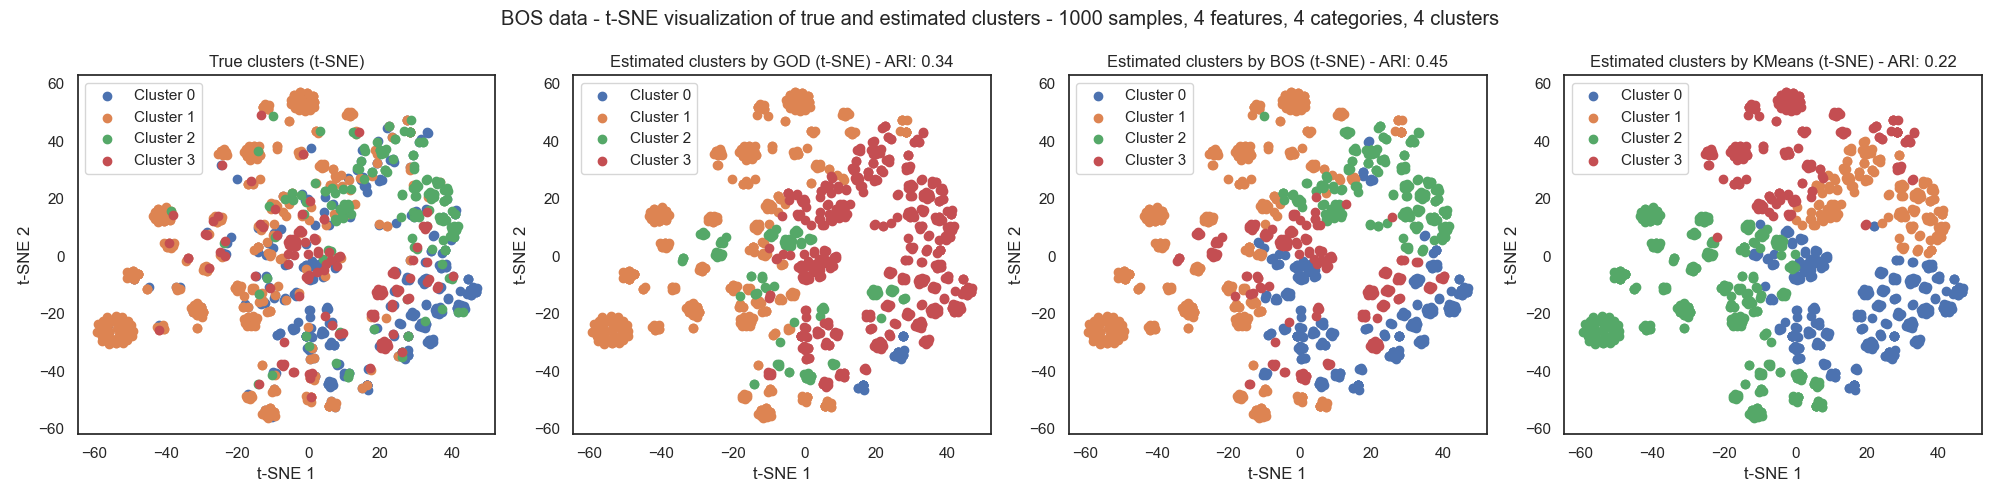
\includegraphics[width=\textwidth]{python_figures/tsne_bos_n1000_d4_m4_k4.png}
        \caption{BOS Model (4 features, 4 Clusters)}
        \label{fig:tsne_bos_4d}
    \end{subfigure}
    \hfill
    \begin{subfigure}[b]{0.49\textwidth}
        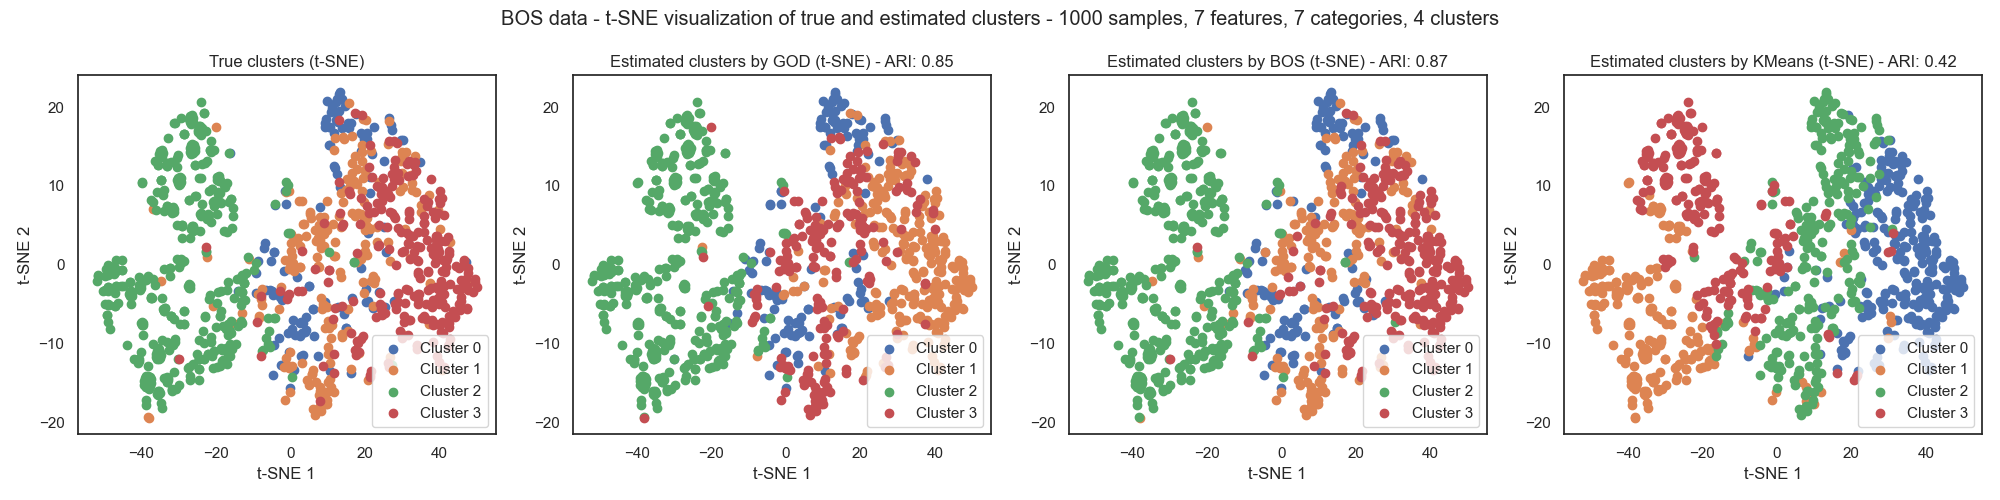
\includegraphics[width=\textwidth]{python_figures/tsne_bos_n1000_d7_m7_k4.png}
        \caption{BOS Model (7 features, 7 Categories)}
        \label{fig:tsne_bos_7d}
    \end{subfigure}
    \newline
    \begin{subfigure}[b]{0.49\textwidth}
        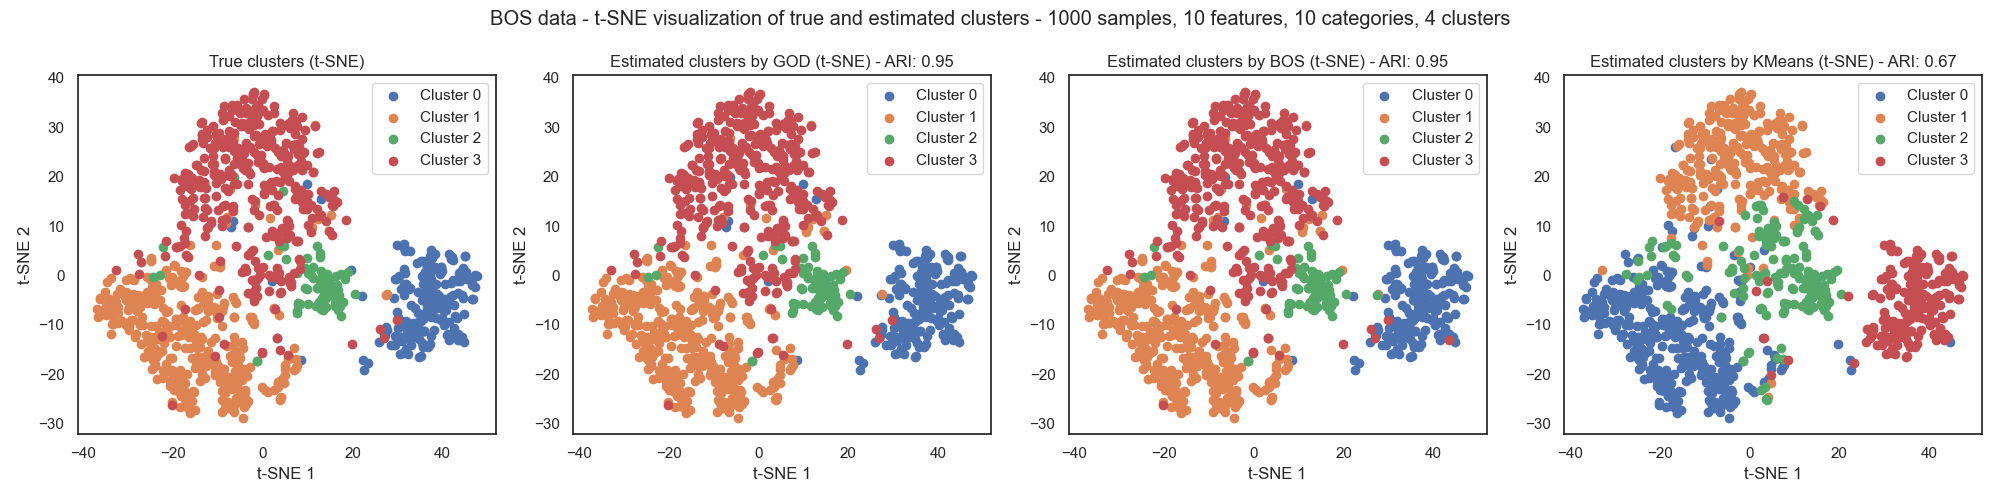
\includegraphics[width=\textwidth]{python_figures/tsne_bos_n1000_d10_m10_k4.png}
        \caption{BOS Model (10 features, 10 Categories)}
        \label{fig:tsne_bos_10d}
    \end{subfigure}
    \hfill
    \begin{subfigure}[b]{0.49\textwidth}
        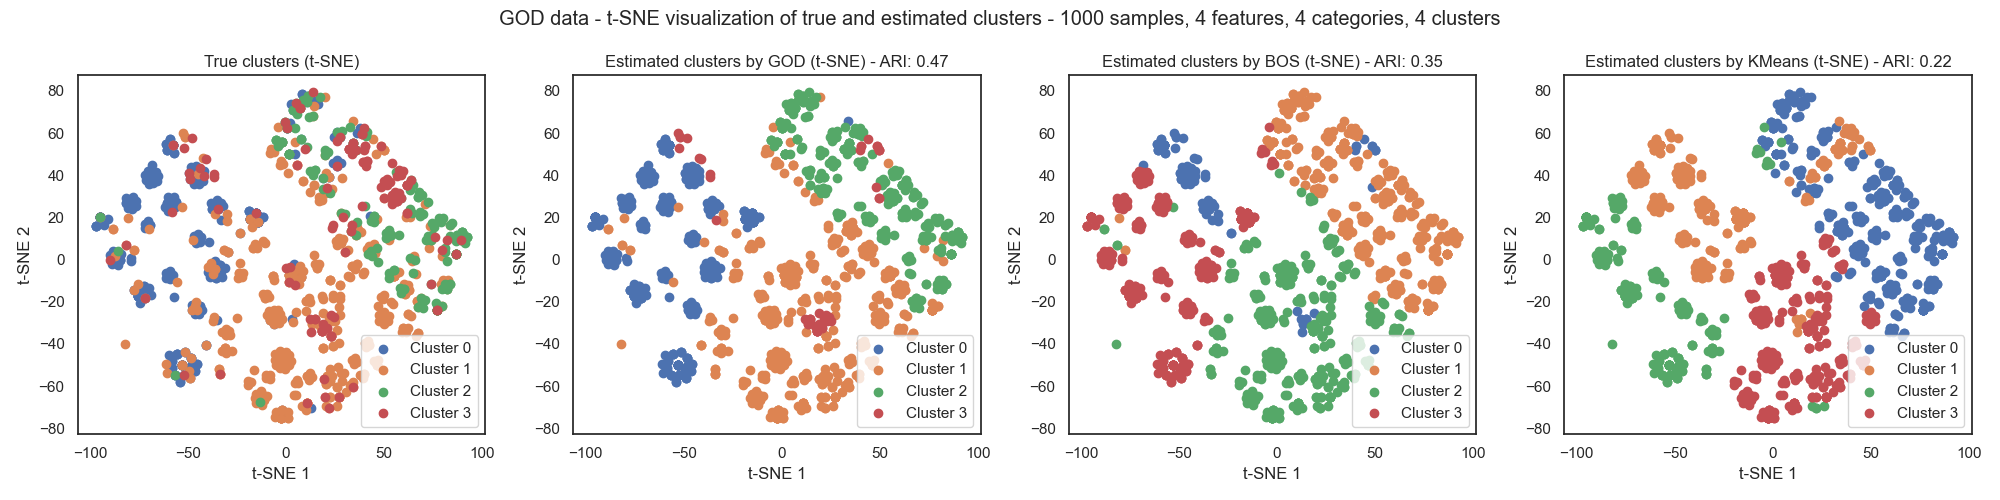
\includegraphics[width=\textwidth]{python_figures/tsne_god_n1000_d4_m4_k4.png}
        \caption{GOD Model (4 features, 4 Clusters)}
        \label{fig:tsne_god_4d}
    \end{subfigure}
    \newline
    \begin{subfigure}[b]{0.49\textwidth}
        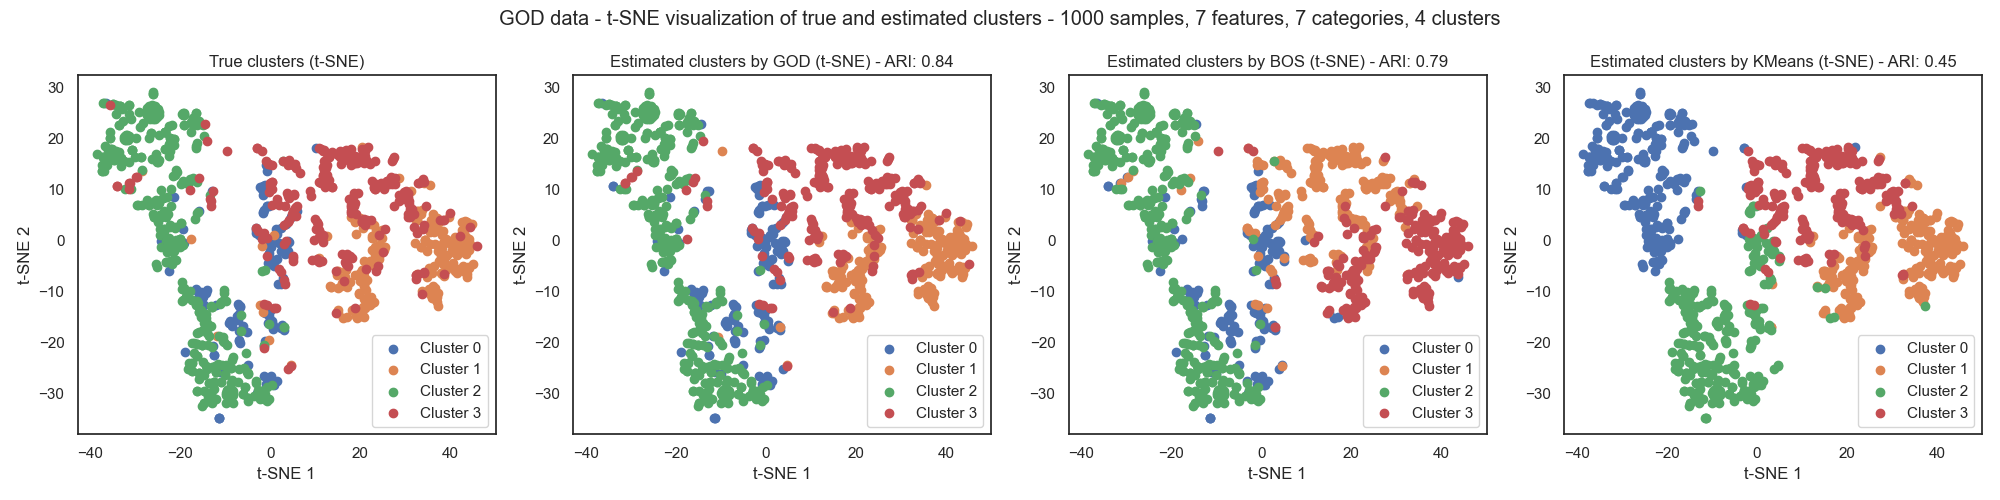
\includegraphics[width=\textwidth]{python_figures/tsne_god_n1000_d7_m7_k4.png}
        \caption{GOD Model (7 features, 7 Clusters)}
        \label{fig:tsne_god_7d}
    \end{subfigure}
    \hfill
    \begin{subfigure}[b]{0.49\textwidth}
        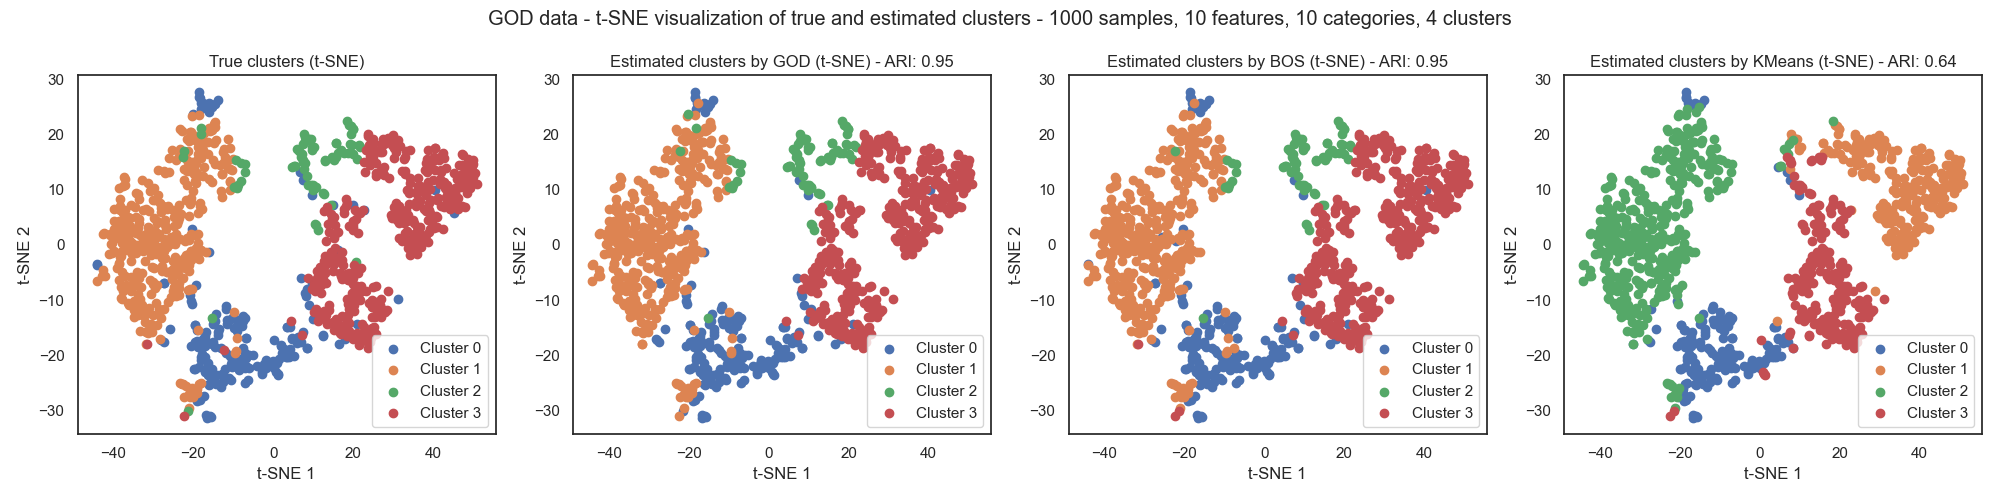
\includegraphics[width=\textwidth]{python_figures/tsne_god_n1000_d10_m10_k4.png}
        \caption{GOD Model (10 features, 10 Clusters)}
        \label{fig:tsne_god_10d}
    \end{subfigure}
    \caption{Comparative t-SNE visualizations and assignment methods analysis. Subfigures (a) and (b) showcase BOS model distributions in 4D and 7D spaces, respectively, highlighting clusters and categories. Subfigure (c) visualizes the GOD model distribution in a 4D space. Subfigure (d) contrasts naive and optimal assignment methods post-clustering. Each visualization underscores the predictive capabilities and clustering accuracy across different dimensions and distributions.}
    \label{fig:tsne_comparative_analysis}
\end{figure}

\section{Real-life datasets}
\label{appendix:metrics_real}

\begin{figure}[H]
    \centering
    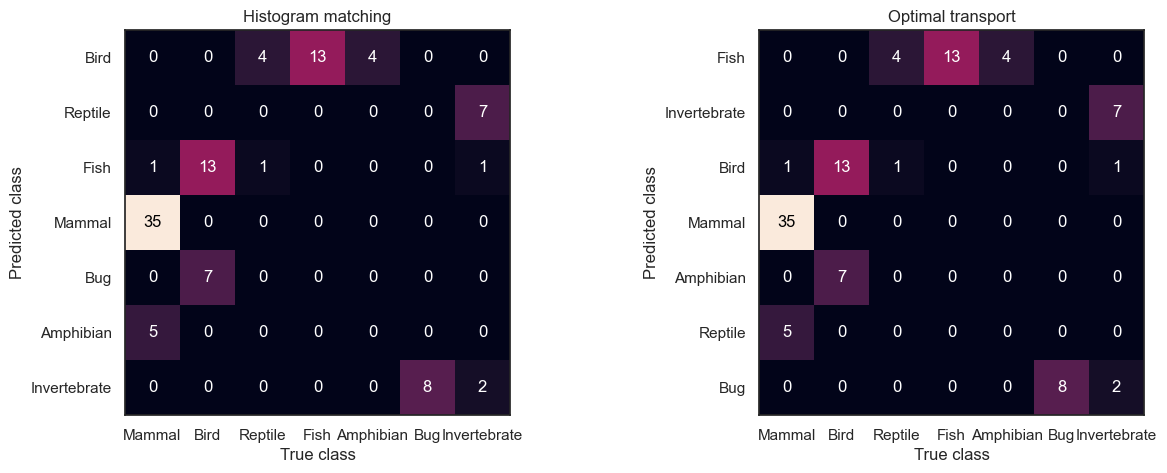
\includegraphics[width=\textwidth]{Attachments/assignment_method.png}
    \caption{Illustration of the two assignment matrices from the different methods after clustering the Zoo dataset. On the left, the naive method and on the right, the optimal assignment method.
    The numbers in the matrices represent the number of samples in the predicted cluster $i$ that are in the true cluster $j$.}
    \label{fig:assignment_methods}
\end{figure}

\begin{table}
\begin{adjustbox}{width=\columnwidth}
\begin{tabular}{lllllll}
\toprule
 &  & \textbf{Runtime (s)} & \textbf{F1} & \textbf{Accuracy} & $W_1$ & \textbf{ARI} \\
Dataset & Method &  &  &  &  &  \\
\midrule
\multirow[t]{6}{*}{\textbf{Zoo}} & \textbf{BOS Random} & 0.93 & 0.89 & 0.89 & 0.20 & 0.85 \\
\textbf{} & \textbf{BOS K-Means} & 0.40 & 0.81 & 0.80 & 0.28 & 0.83 \\
\textbf{} & \textbf{GOD Random} & 0.63 & \textbf{\underline{0.90}} & \textbf{\underline{0.90}} & \textbf{\underline{0.08}} & \textbf{\underline{0.91}} \\
\textbf{} & \textbf{GOD K-Means} & 0.25 & 0.81 & 0.80 & 0.28 & 0.83 \\
\textbf{} & \textbf{K-Means} & \textbf{\underline{0.01}} & 0.84 & 0.85 & 0.20 & 0.83 \\
\textbf{} & \textbf{Gaussian} & 0.52 & 0.77 & 0.74 & 0.55 & 0.66 \\
\cline{1-7}
    \multirow[t]{6}{*}{\textbf{Car Evaluation}} & \textbf{BOS Random} & 0.20 & 0.46 & 0.38 & \textbf{\underline{0.72}} & 0.01 \\
    \textbf{} & \textbf{BOS K-Means} & 0.52 & 0.45 & 0.38 & 1.01 & \textbf{\underline{0.04}} \\
\textbf{} & \textbf{GOD Random} & 0.18 & \textbf{\underline{0.48}} & \textbf{\underline{0.42}} & 0.74 & -0.00 \\
\textbf{} & \textbf{GOD K-Means} & 0.60 & 0.39 & 0.31 & 1.03 & -0.00 \\
    \textbf{} & \textbf{K-Means} & \textbf{\underline{0.01}} & 0.35 & 0.29 & 1.11 & 0.00 \\
\textbf{} & \textbf{Gaussian} & 0.04 & 0.41 & 0.33 & 1.24 & 0.01 \\
\cline{1-7}
    \multirow[t]{6}{*}{\textbf{Hayes-Roth}} & \textbf{BOS Random} & 0.09 & \textbf{\underline{0.45}} & \textbf{\underline{0.46}} & 0.14 & 0.02 \\
\textbf{} & \textbf{BOS K-Means} & 0.09 & 0.34 & 0.33 & 0.16 & -0.01 \\
\textbf{} & \textbf{GOD Random} & 0.26 & 0.40 & 0.41 & 0.34 & 0.01 \\
\textbf{} & \textbf{GOD K-Means} & 0.06 & 0.36 & 0.36 & 0.22 & -0.01 \\
\textbf{} & \textbf{K-Means} & \textbf{\underline{0.00}} & 0.34 & 0.33 & 0.16 & -0.01 \\
\textbf{} & \textbf{Gaussian} & 0.03 & \textbf{\underline{0.45}} & 0.45 & \textbf{\underline{0.11}} & \textbf{\underline{0.07}} \\
\cline{1-7}
    \multirow[t]{6}{*}{\textbf{Caesarian}} & \textbf{BOS Random} & 0.26 & \textbf{\underline{0.61}} & \textbf{\underline{0.64}} & 0.21 & \textbf{\underline{0.06}} \\
\textbf{} & \textbf{BOS K-Means} & 0.15 & 0.54 & 0.54 & 0.09 & -0.01 \\
\textbf{} & \textbf{GOD Random} & 0.24 & 0.57 & 0.57 & 0.23 & 0.01 \\
\textbf{} & \textbf{GOD K-Means} & 0.12 & 0.56 & 0.56 & 0.06 & 0.00 \\
    \textbf{} & \textbf{K-Means} & \textbf{\underline{0.00}} & 0.56 & 0.56 & 0.09 & 0.00 \\
    \textbf{} & \textbf{Gaussian} & 0.02 & 0.59 & 0.59 &\textbf{\underline{0.04}} & 0.02 \\
\cline{1-7}
    \multirow[t]{6}{*}{\textbf{Nursery}} & \textbf{BOS Random} & \textbf{\underline{0.91}} & \textbf{\underline{0.40}} & \textbf{\underline{0.42}} & 0.84 & 0.04 \\
\textbf{} & \textbf{BOS K-Means} & 1.30 & 0.32 & 0.29 & 0.30 & 0.01 \\
    \textbf{} & \textbf{GOD Random} & 5.31 & 0.40 & 0.39 & \textbf{\underline{0.26}} & 0.03 \\
\textbf{} & \textbf{GOD K-Means} & 3.97 & 0.31 & 0.28 & 0.71 & 0.01 \\
    \textbf{} & \textbf{K-Means} & 1.42 & 0.36 & 0.31 & 0.47 & \textbf{\underline{0.07}} \\
\textbf{} & \textbf{Gaussian} & 33.32 & 0.34 & 0.29 & 0.54 & 0.05 \\
\cline{1-7}
\bottomrule
\end{tabular}
\end{adjustbox}
\caption{
Results of the classification task for the different datasets and the proposed methods. The metrics are the F1-score, the accuracy, the Wasserstein distance and the adjusted rand index (ARI). 
The runtime is also reported. The best results for each dataset and metric are highlighted in bold italic and underlined. 
}
\label{tab:results_real}
\end{table}

%\tm{Penser à mettre en avant les bons résultats. Eventuellement ajouter les temps de calcul}

\subsection*{t-SNE plots}
\label{sec:appendix_tsne}

\begin{figure}[H]
    \centering
    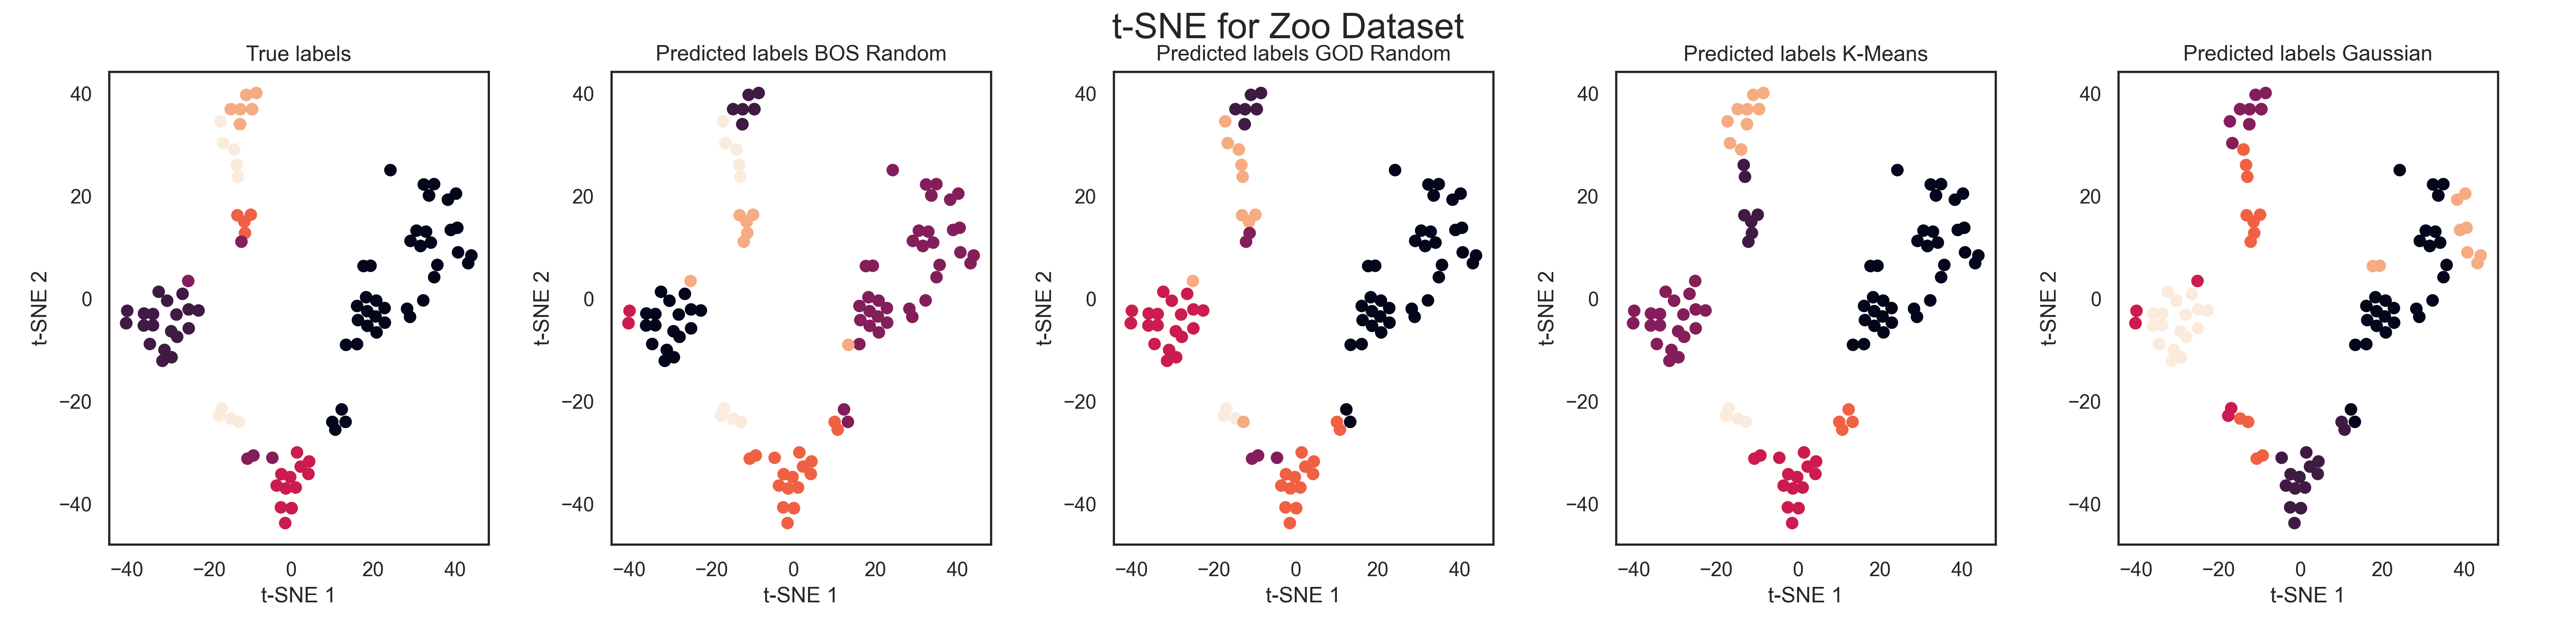
\includegraphics[width=\textwidth]{python_figures/tsne_zoo.png}
    \caption{t-SNE visualization of the Zoo dataset with the true labels and the predicted clusters for the BOS model with random initialization, the GOD model with random initialization, the K-Means algorithm and the Gaussian Mixture Models.}
    \label{fig:tsne_zoo}
\end{figure}

\begin{figure}[H]
    \centering
    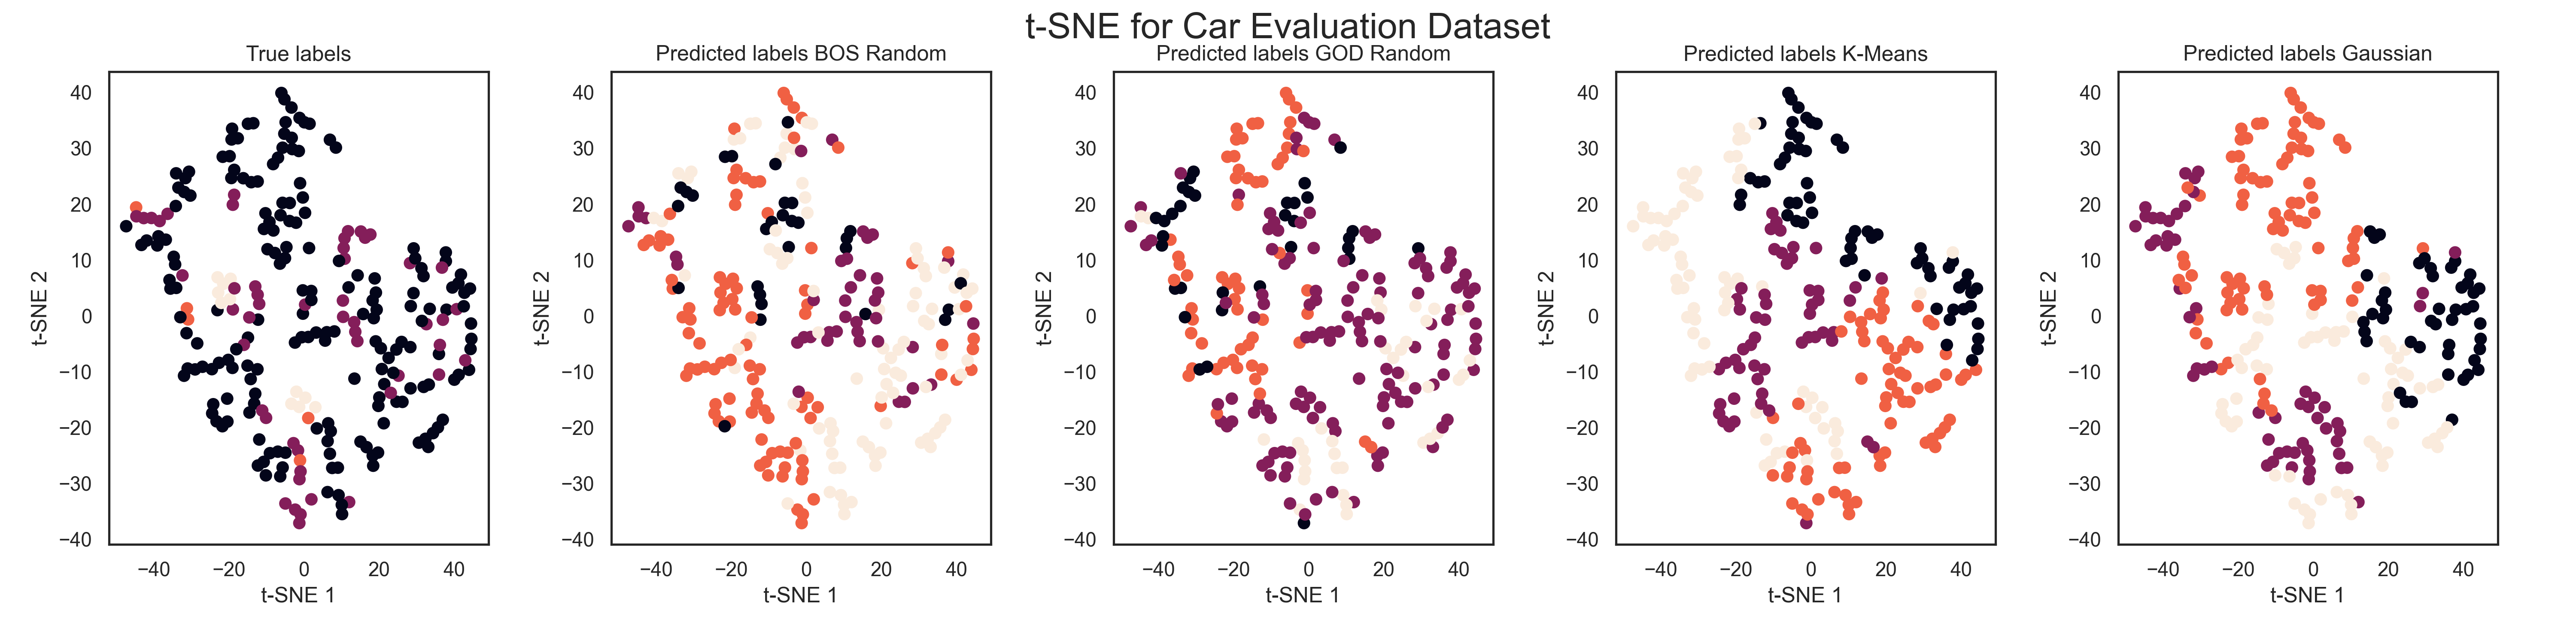
\includegraphics[width=\textwidth]{python_figures/tsne_car_evaluation.png}
    \caption{t-SNE visualization of the Car Evaluation dataset with the true labels and the predicted clusters for the BOS model with random initialization, the GOD model with random initialization, the K-Means algorithm and the Gaussian Mixture Models.}
    \label{fig:tsne_car}
\end{figure}

\begin{figure}[H]
    \centering
    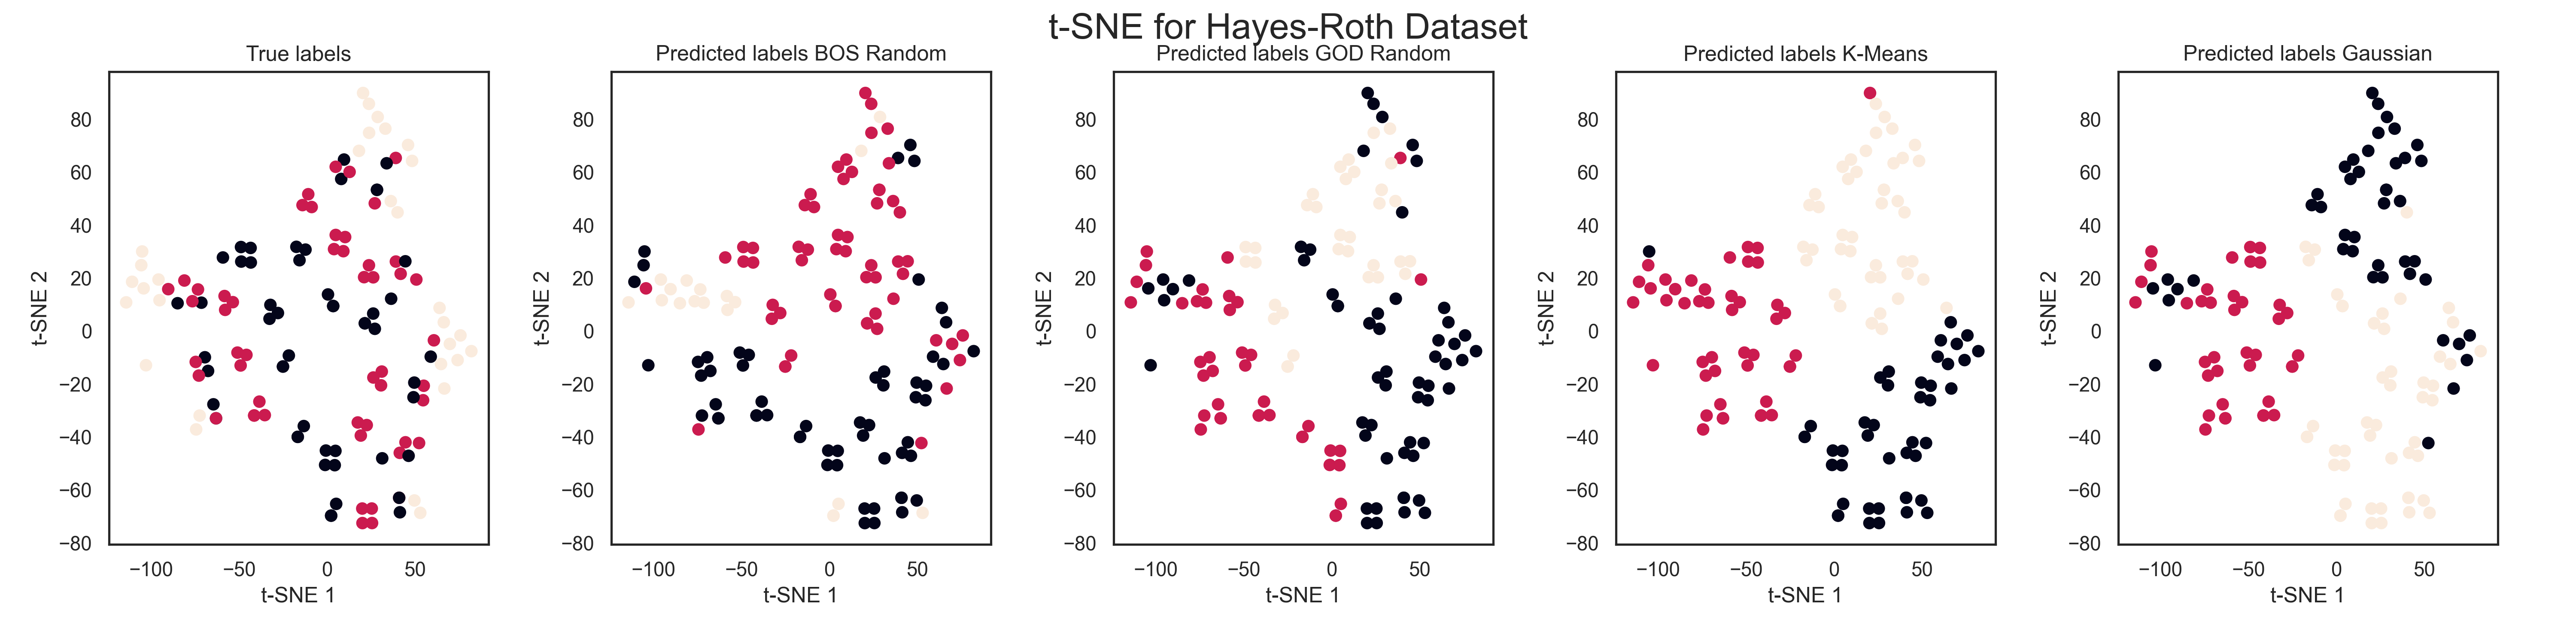
\includegraphics[width=\textwidth]{python_figures/tsne_hayes-roth.png}
    \caption{t-SNE visualization of the Hayes-Roth dataset with the true labels and the predicted clusters for the BOS model with random initialization, the GOD model with random initialization, the K-Means algorithm and the Gaussian Mixture Models.}
    \label{fig:tsne_hr}
\end{figure}

\begin{figure}[H]
    \centering
    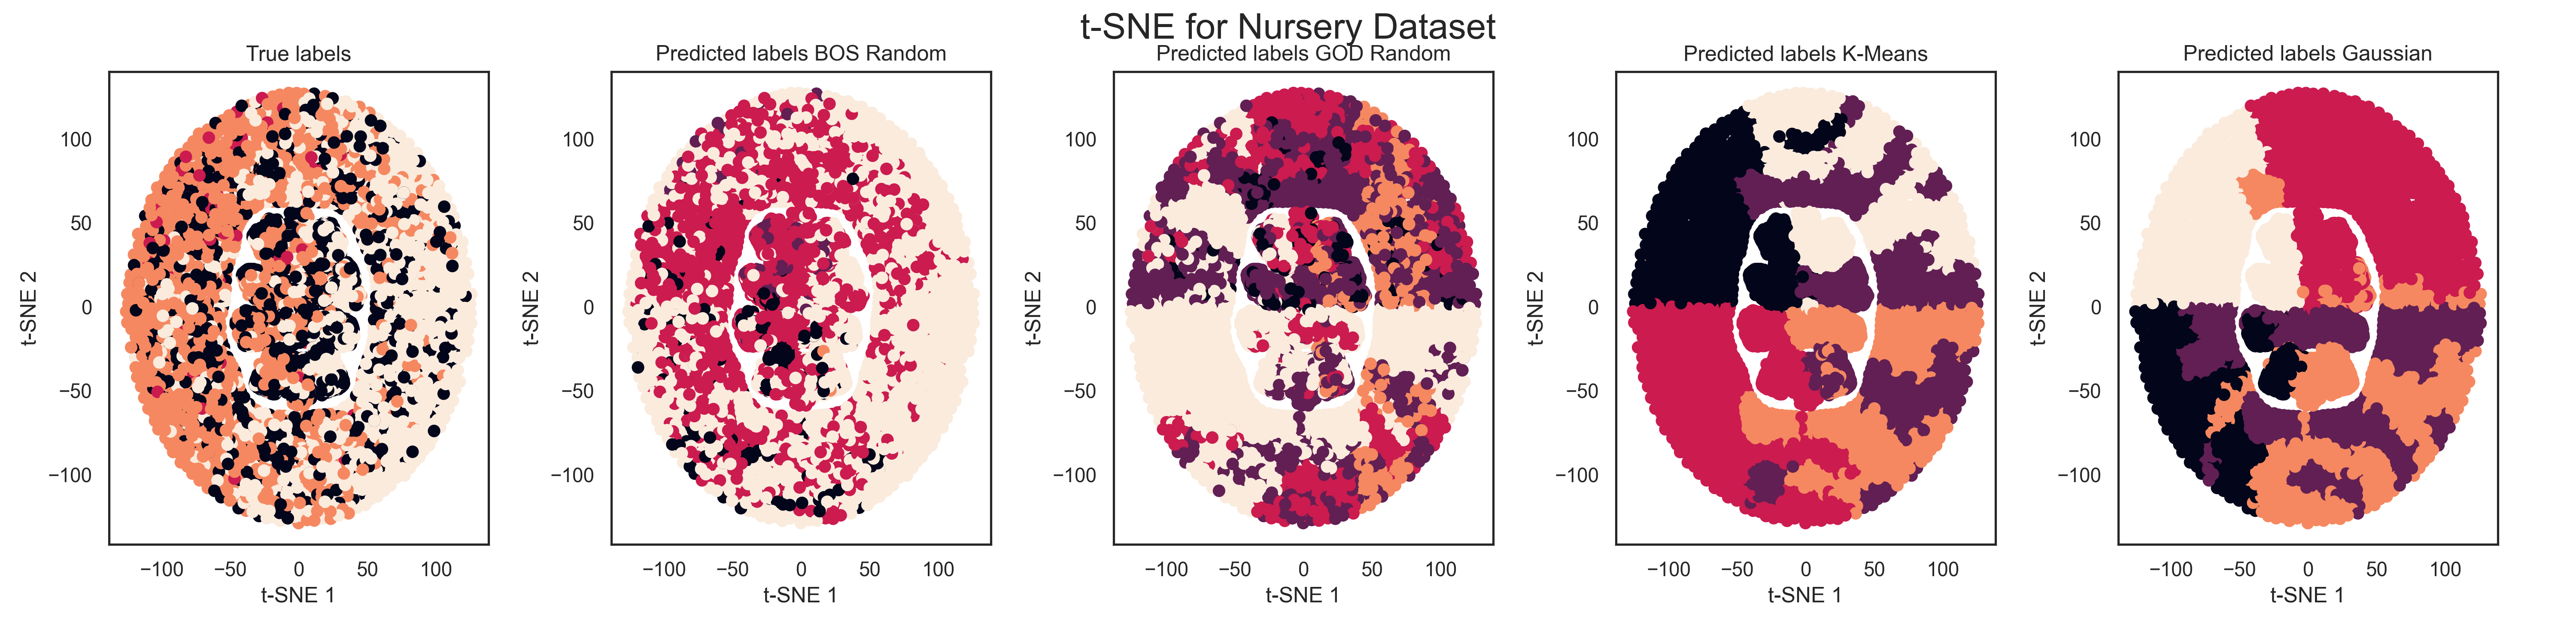
\includegraphics[width=\textwidth]{python_figures/tsne_nursery.png}
    \caption{t-SNE visualization of the Nursery School dataset with the true labels and the predicted clusters for the BOS model with random initialization, the GOD model with random initialization, the K-Means algorithm and the Gaussian Mixture Models. While continuous clustering algorithms separate the circle as expected, categorical algorithms are a little more subtle and adapted.}
    \label{fig:tsne_hr}
\end{figure}

% \begin{figure}[H]
%     \centering
%     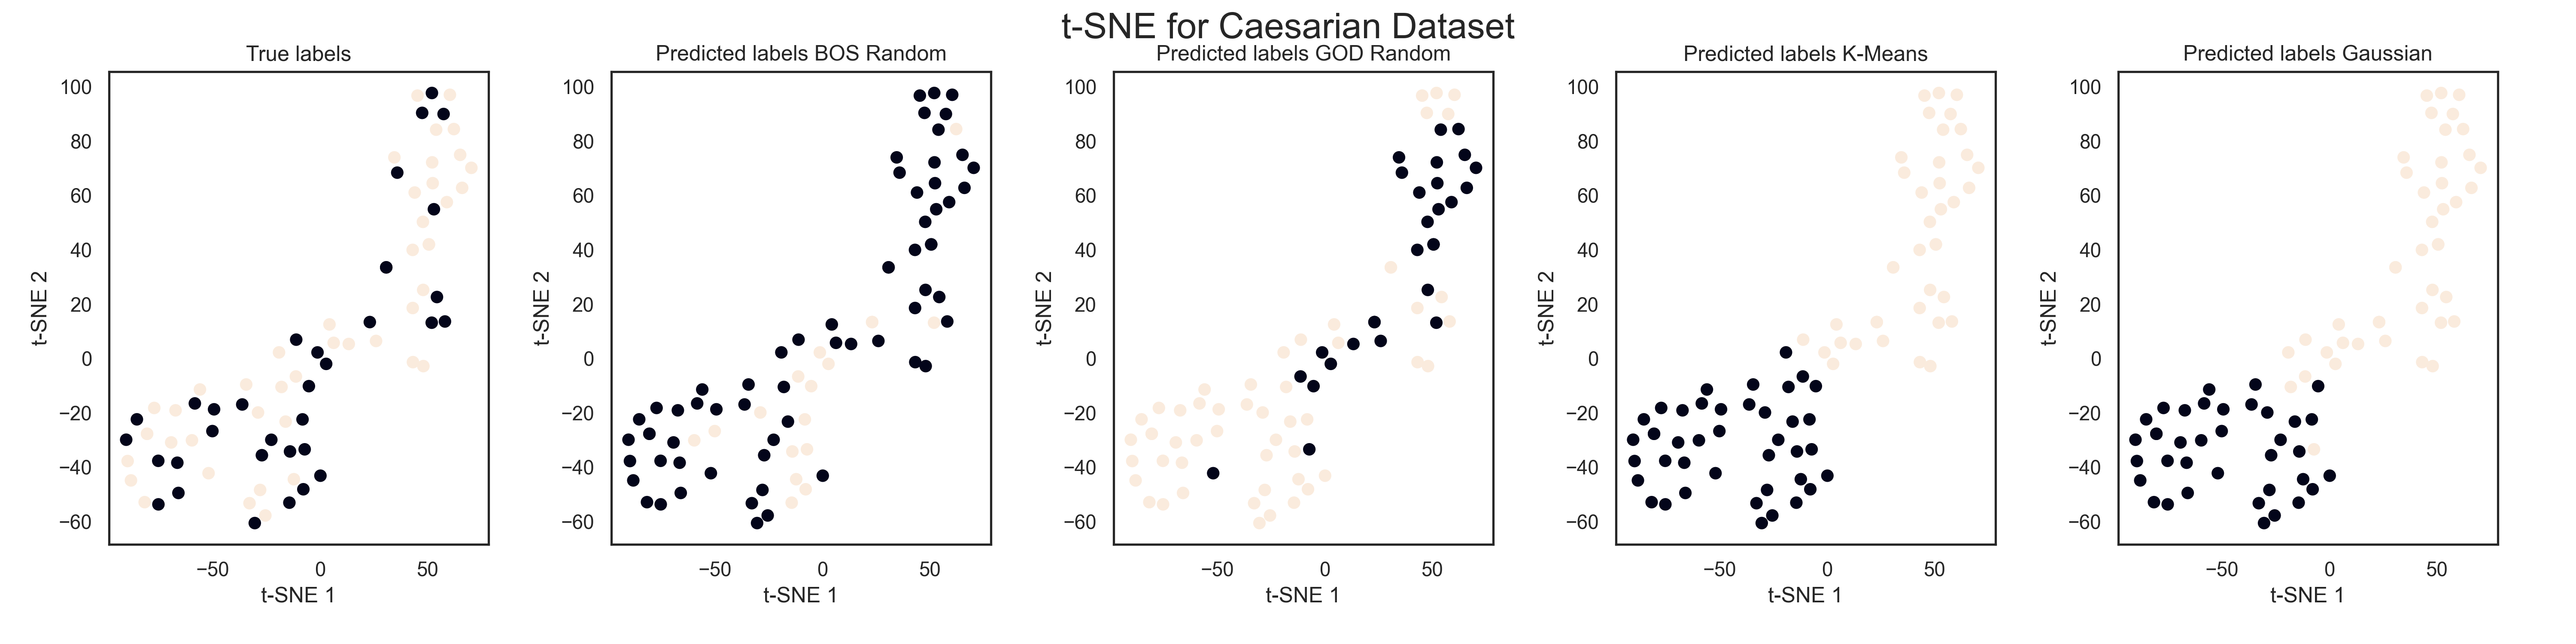
\includegraphics[width=\textwidth]{python_figures/tsne_caesarian.png}
%     \caption{t-SNE visualization of the Caesarian dataset with the true labels and the predicted clusters for the BOS model with random initialization, the GOD model with random initialization, the K-Means algorithm and the Gaussian Mixture Models.}
%     \label{fig:tsne_caesarian}
% \end{figure}

\subsection*{Assignment matrix and histograms}
\label{sec:appendix_assign}

\begin{figure}[H]
    \centering
    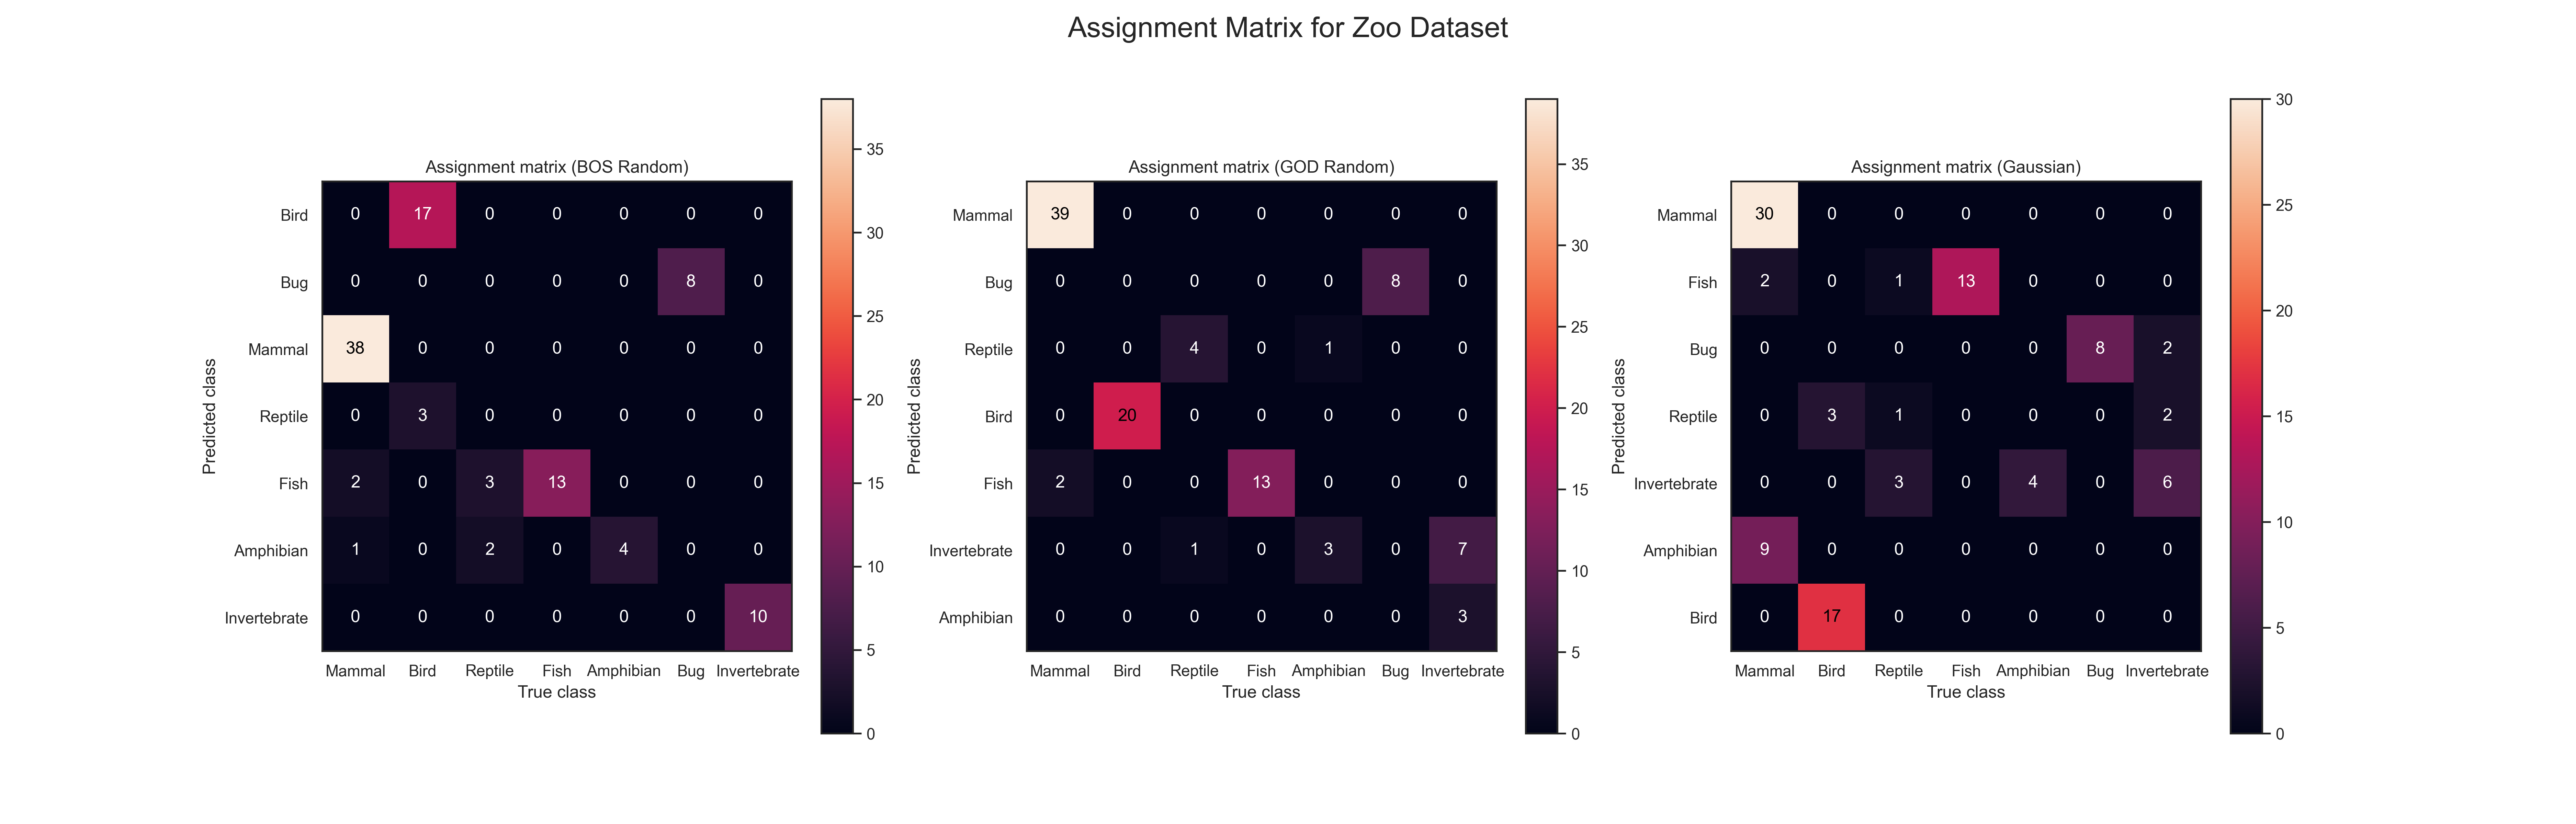
\includegraphics[width=\linewidth]{python_figures/assignment_matrix_zoo.png}
    \caption{Assignment matrix for the Zoo dataset with different methods.}
    \label{fig:assign_zoo}
\end{figure}

\begin{figure}[H]
    \centering
    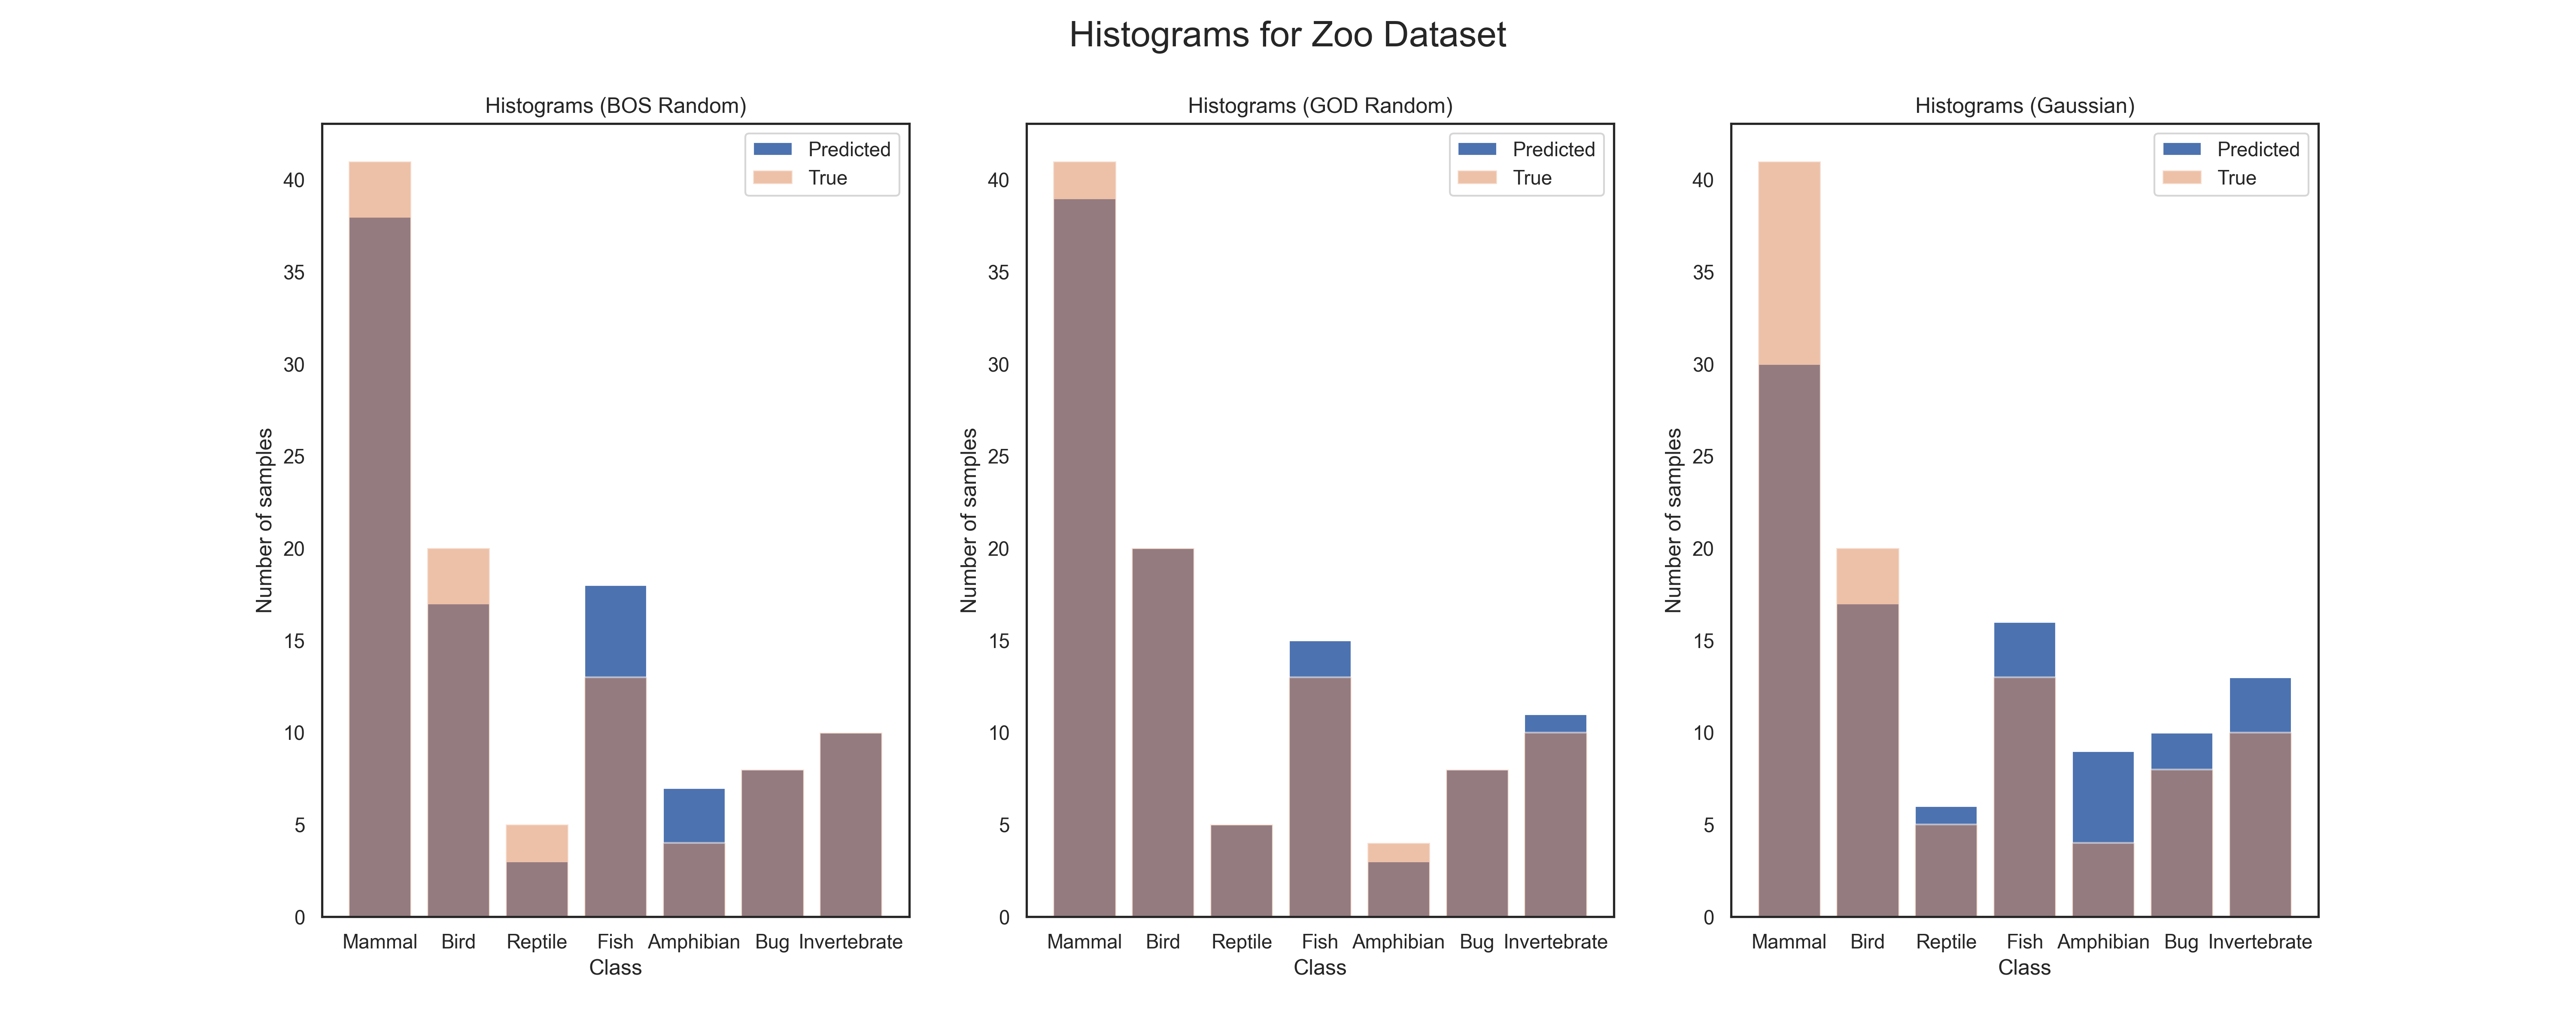
\includegraphics[width=\linewidth]{python_figures/histograms_zoo.png}
    \caption{Histograms for the Zoo dataset with different methods.}
    \label{fig:hist_zoo}
\end{figure}


\section{Generic proofs}

\subsection{Ternary search algorithm}
\label{sec:ternary_search_algorithm}

\begin{algorithm}[H]
    \caption{Ternary search}
    \begin{algorithmic}[1]
    \Require $f$ concave on $[a, b]$, $\epsilon > 0$
    \Ensure For $y$ the returned value, $\exists x \in \argmax_{[a, b]} f$, $|y - x| < \epsilon$
    
    \Function{TernarySearch}{$f$, $a$, $b$, $\epsilon$}

    \If {$b - a < \epsilon$}
        \State \Return $\frac{a + b}{2}$
    \EndIf
    
    \State $c \leftarrow a + \frac{b - a}{3}$
    \State $d \leftarrow a + \frac{2(b - a)}{3}$
    
    \If {$f(c) \geq f(d)$}
        \State \Return \Call{TernarySearch}{$f$, $a$, $d$, $\epsilon$}
    \Else
        \State \Return \Call{TernarySearch}{$f$, $c$, $b$, $\epsilon$}
    \EndIf
    \EndFunction
    
    \end{algorithmic}
\end{algorithm}


\begin{thm}
    Let $f$ be a concave function on $[A, B]$. The ternary search algorithm returns a value $y$ such that $\exists x \in \argmax_{[A, B]} f$, $|y - x| < \epsilon$.
\end{thm}
\begin{proof}
    The algorithm stops when the length of the interval is less than $\epsilon$. At each iteration, the length of the interval is multiplied by $\frac{2}{3}$. Hence the algorithm terminates and require $\Theta(\log \frac{b - a}{\epsilon})$ iterations.

    \tr{TODO: clean this} 
    Indeed after iteration $k$, the length of the interval is $\left(\frac{2}{3}\right)^k(b - a)$~\footnote{$\lg=\log_2$}:
    \begin{align}
        \left(\frac{2}{3}\right)^k(b - a) < \epsilon &\Leftrightarrow \left(\frac{2}{3}\right)^k < \frac{\epsilon}{b - a} \\
        &\Leftrightarrow k (\lg 2 - \lg 3) < \lg \frac{\epsilon}{b - a} \\
        &\Leftrightarrow k > \frac{1}{\lg 3 - 1} \lg \frac{b - a}{\epsilon}
        \end{align}
    which for $\epsilon = 2^{-p}$ and $b - a \leq 1$ gives:
    \begin{equation}
        k > \frac{1}{\lg 3 - 1} p \approx 1.7095 p
    \end{equation}

    We note $[a, b]$ the interval on which the algorithm is called and $[A, B]$ the initial interval.
    We prove the following invariant: at each iteration of the algorithm, the interval $[a, b]$ is such that $\exists x \in \argmax_{[a, b]} f, a \leq x \leq b$.
    \begin{itemize}
        \item At the beginning of the algorithm, we have $a = A$ and $b = B$. The invariant is true.
        \item We now suppose that $f(c) \geq f(d)$. We want to prove that the invariant is true for the interval $[a, d]$. We just have to prove that for any $g \in ]d, b]$, $f(g) \leq f(c)$ (\text{i.e.} $g$ is not an argmax or if so $c$ is alos one). As $d \in [c, g]$, we have $\lambda \in ]0, 1]$ such that $g = (1 - \lambda)c + \lambda d$. As $f$ is concave, we have $f(d) \geq (1 - \lambda)f(c) + \lambda f(g)$. As $f(c) \geq f(d)$, we have $f(c) - (1 - \lambda)f(c) \geq \lambda f(g)$ which gives $f(c) \geq f(g)$. Hence the invariant is true for the interval $[a, d]$.
        
        We can do the same reasoning for the case $f(c) < f(d)$ and the interval $[c, b]$.
    \end{itemize}
\end{proof}


\subsection{Concavity}

\begin{lemma}[Concavity of log composed functions]
    \label{lemma:concavity_log_composed_functions}
    For $f: I \rightarrow \RR_+^*$ be a twice-differentiable function, we have that:
    \[ \ln \circ f \text{ is concave } \iff  f'^2 - f f'' \geq 0 \]
\end{lemma}
\begin{proof}
    We have that:
    \begin{align}
        (\ln \circ f)' &= \frac{f'}{f}\\
        (\ln \circ f)'' &= \frac{f''f - f'^2}{f^2}
    \end{align}
    
    Therefore, $\ln \circ f$ is concave if and only if $f'^2 - f f'' \geq 0$.
\end{proof}


\section{BOS Model proofs}
\label{appendix:bos_proofs}

\subsection{Notations}

For the whole section we will consider that $e$ is a subset of $\bbrack{1, m}$ and that supposing that we know $e$ means that we look a the random process where the starting set of categories is $e$. We will also note $e^{-,y}$, $e^{=,y}$ and $e^{+,y}$ the sets of categories that are respectively less than, equal to and greater than $y$ in $e$ and $f$ any next set of categories considered in the BOS process. For example,  $\Pr(f | e)$ is the probability of having as next set of categories $f$ knowing that the current set of categories is $e$ (you could imagine that we have $j$ such that $e_j = e$ and $e_{j+1} = f$).

\begin{definition}
    We define $\correct{\mu}{e}{y}{f}$ as the indicator function that $f$ is the correct subset to choose in case of a perfect comparison \textit{i.e.} if $\mu \in f$ or by default the closest to $\mu$.
\end{definition}

\begin{definition}
    We define $\nextes{e}{y}$ as the set of intervals that can be chosen after a comparison at breakpoint $y$ in the interval $e$ \textit{i.e.} $\nextes{e}{y} = \set{e^{-,y}, e^{=,y}, e^{+,y}}$ with $e = \bbrack{l, u - 1}$ and $y \in \bbrack{l, u - 1}$: $e^{-,y} = \bbrack{l, y - 1}$, $e^{=,y} = \set{y}$ and $e^{+,y} = \bbrack{y + 1, u - 1}$.
\end{definition}


\subsection{Polynomiality}

\begin{lemma}[Transition probability]
    \label{lemma:bos_transition}
    $\forall m \in \NN^*, \forall x \in \bbrack{1, m}, \forall \mu \in \bbrack{1, m}, \pi \in [0, 1], \forall e \subset \bbrack{1, m}, \forall f \subset e$:
    \[ \Pr(f | x \in e, e, \mu, \pi) =  \frac{1}{\card{e}}  \sum_{y \in e} \left[ \left( \correct{\mu}{e}{y}{f} - \frac{\card{f}}{\card{e}} \right) \pi + \frac{\card{f}}{\card{e}} \right]  \indickronecker{x \in \nextes{e}{y}} \]

    Note that $\indickronecker{x \in \nextes{e}{y}} = 1$ only for one value of $y$ and $0$ for all the others. Moreover $\pi \mapsto \Pr(f | x \in e, e, \mu, \pi)$ is an affine function.
\end{lemma}
\begin{proof}
    We have that, by marginalization over the breakpoint $y$:
    \begin{align}
        \Pr(f | x \in e, e, \mu, \pi) 
        &= \sum_{y \in e} \Pr(f, y | x \in e, e, \mu, \pi) \\
        &= \sum_{y \in e} \Pr(f | y, x \in e, e, \mu, \pi) \Pr(y | x \in e, e, \mu, \pi) \\
        &= \sum_{y \in e} \Pr(f | y, x \in e, e, \mu, \pi) \frac{1}{\card{e}} \\
        &= \frac{1}{\card{e}} \sum_{y \in e} \Pr(f | y, x \in e, e, \mu, \pi)
    \end{align}

    Then by marginalization over the accuracy indicator $z$:
    \begin{align}
        \Pr(f | x \in e, e, \mu, \pi) 
        &= \frac{1}{\card{e}} \sum_{y \in e} \sum_{z \in \set{0, 1}} \Pr(f | y, x \in e, e, \mu, \pi, z) \Pr(z | y, x \in e, e, \mu, \pi) \\
        &= \frac{1}{\card{e}} \sum_{y \in e} \left[ \Pr(f | y, x \in e, e, \mu, \pi, z=1) \pi + \Pr(f | y, x \in e, e, \mu, \pi, z=0) (1 - \pi) \right] \\
        &= \frac{1}{\card{e}}  \sum_{y \in e} \left[ \correct{\mu}{e}{y}{f} \pi + \frac{\card{f}}{\card{e}} (1 - \pi) \right]  \indickronecker{x \in \nextes{e}{y}} \\
        &= \frac{1}{\card{e}}  \sum_{y \in e} \left[ \left( \correct{\mu}{e}{y}{f} - \frac{\card{f}}{\card{e}} \right) \pi + \frac{\card{f}}{\card{e}} \right]  \indickronecker{x \in \nextes{e}{y}}
    \end{align}
\end{proof}

\begin{lemma}
    \label{lemma:bos_polynomial}
    $\forall m \in \NN^*, \forall x \in \bbrack{1, m}, \forall \mu \in \bbrack{1, m}, \pi \in [0, 1], \forall e \subset \bbrack{1, m}$:
    \[ \pi \mapsto \Pr(x | x \in e, e, \mu, \pi)\] 
    is a polynomial function of degree at most $\card{e} - 1$.
\end{lemma}
\begin{proof}
    Let $m \in \NN^*, x \in \bbrack{1, m}, \mu \in \bbrack{1, m}, \pi \in [0, 1]$.

    We proceed by strong induction on $\card{e}$.
    \begin{itemize}
        \item Initialization: $\card{e} = 1$:
        \[ \Pr(x | x \in e, e, \mu, \pi) = \indickronecker{e = \set{x}} \] which is a polynomial function of degree $0$.
        
        \item Induction: Suppose the result holds for all $f \subset \bbrack{1, m}$ of size less or equal than $\card{e} - 1$ and let us prove it for $\card{e}$.
        
        We marginalize over the next interval $f$ and we have that:
        \begin{align}
            \Pr(x | x \in e, e, \mu, \pi) 
            &= \sum_{f \subset e} \Pr(x, f | x \in e, e, \mu, \pi) \\
            &= \sum_{f \subset e} \Pr(x | f, x \in e, e, \mu, \pi) \Pr(f | x \in e, e, \mu, \pi)
        \end{align}

        We can then notice that $\Pr(x | f, x \in e, e, \mu, \pi)$ is $0$ if $x \notin f$ and that $e$ does not intervene in the BOS process anymore. Hence we can replace $\Pr(x | f, x \in e, e, \mu, \pi)$ by $\Pr(x | x \in f, f, \mu, \pi)$ and sum only over $f \subset e$ such that $x \in f$:

        \begin{align}
            \Pr(x | x \in e, e, \mu, \pi) 
            &= \sum_{f \subset e ; x \in f} \Pr(x | x \in f, f, \mu, \pi) \Pr(f | x \in e, e, \mu, \pi)
        \end{align}

        As $\Pr(f | x \in e, e, \mu, \pi)$ is a polynomial function of degree at most $1$ (see lemma \ref{lemma:bos_transition}) and $\Pr(x | f, x \in f, f, \mu, \pi)$ is a polynomial function of degree at most $\card{f} - 1 \leq \card{e} - 2$ by induction hypothesis, we have that $\Pr(x | x \in e, e, \mu, \pi)$ is a polynomial function of degree at most $\card{e} - 1$.
    \end{itemize}

    Hence the result holds for all $e$.
\end{proof}


\begin{thm}[Likelihood is polynomial]
    \label{thm:likelihood_bos_is_polynomial}
    $\forall m \in \NN^*, \forall x \in \bbrack{1, m}, \forall \mu \in \bbrack{1, m}$,:
    \[ \pi \mapsto \Pr(x | \mu, \pi) \]
    is a polynomial function of degree at most $m - 1$.  
\end{thm}
\begin{proof}
    Let $m \in \NN^*$, $x \in \bbrack{1, m}$ and $\mu \in \bbrack{1, m}$. 

    First we can introduce redondant knowledge as we start necessarily with the full set of categories, we can add its value as known. We have that $\Pr(x | \mu, \pi) = \Pr(x | e_1, \mu, \pi)$. We also now that $x \in e_1$ therefore $\Pr(x | \mu, \pi) = \Pr(x | x \in e_1, e_1, \mu, \pi)$.

    We can now use the previous lemma~\ref{lemma:bos_polynomial} to conclude that $\Pr(x | \mu, \pi)$ is a polynomial function of degree at most $m - 1$.
\end{proof}


\subsection{Concavity}

% We can now prove that $\forall x \in \bbrack{0, h - 1}, \forall \mu \in \bbrack{0, h - 1}, \pi \mapsto \Pr(x | x \in \bbrack{0, h - 1}, \mu, \pi)$ is concave on $[0, 1]$
% 
% 
% \begin{lemma}[Log concavity affine times polynomial]
%     \label{lemma:concavity_log_polynomial_times_affine}
%     For $I$ a real interval.
% 
%     Let $P$ be a $\log$-concave function on $I$ and $a, b \in \RR$ with $\forall t  \in I, at + b \geq 0$. Then $f: t \mapsto (at + b)P(t)$ is $\log$-concave on $I$.
% \end{lemma}
% \begin{proof}
%     Let $t \in I$.
% 
%     As $at + b \geq 0$, we have that $f(t) \geq 0$. We can therefore consider its logarithm (with that $\log(0) = -\infty$).
% 
%     We have that:
%     \begin{align}
%         f'(t) &= aP(t) + (at + b)P'(t) \\
%         f''(t) &= 2 aP'(t) + (at + b)P''(t) \\
%         f'(t)^2 &= a^2P(t)^2 + 2a(at + b)P(t)P'(t) + (at + b)^2P'(t)^2 \\
%         f(t)f''(t) &= 2a(at + b) P(t)P'(t) + (at + b)^2P(t)P''(t)
%     \end{align}
% 
%     Hence:
%     \[f'(t)^2 - f(t) f''(t) = a^2 P(t)^2 + (at + b)^2 \left[ P'(t)^2 - P(t)P''(t) \right] \]
% 
%     As $P$ is $\log$-concave on $I$, using the lemma~\ref{lemma:concavity_log_composed_functions} we have that $P'(t)^2 - P(t)P''(t) > 0$.
%     
%     As all the terms are $\geq 0$ we have that $\forall t \in I, f'(t)^2 - f(t) f''(t) \geq 0$ and using the lemma~\ref{lemma:concavity_log_composed_functions} we have that $f$ is $\log$-concave on $I$.
% \end{proof}
% 
% \begin{lemma}[Log concavity of the BOS model]
%     \label{lemma:log_concavity_bos_model}
%     $\forall m \in \NN^*, \forall x \in \bbrack{1, m}, \forall \mu \in \bbrack{1, m},, \forall e \subset \bbrack{1, m}$:
%     \[ \pi \mapsto \Pr(x | x \in e, e, \mu, \pi) \]
%     is $\log$-concave on $[0, 1]$.
% \end{lemma}
% \begin{proof}
%     Let $m \in \NN^*$, $x \in \bbrack{1, m}$ and $\mu \in \bbrack{1, m}$.
%     We proceed by induction on $\card{e}$:
% 
%     \[ P_n : \forall e \subset \bbrack{1, m}, |e| \leq n \Rightarrow \pi \mapsto \Pr(x | x \in e, e, \mu, \pi) \text{ is } \log\text{-concave on } [0, 1] \]
% 
%     \begin{itemize}
%         \item Initialization: $\card{e} = 1$:
%         \[\pi \mapsto \Pr(x | x \in e, e, \mu, \pi) = \indickronecker{e = \set{x}} \] which is $\log$-concave on $[0, 1]$.
%         Thus $P_1$ holds.
% 
%         \item Induction: Suppose $P_n$, the result holds for all $f \subset \bbrack{1, m}$ of size less or equal than $n$ and let us prove it for $n+1$.
%         
%         Let $e \subset \bbrack{1, m}$ such that $\card{e} = n + 1$.
% 
%         Using the lemma~\ref{lemma:bos_polynomial}, we have:
%         \begin{align}
%             \Pr(x | x \in e, e, \mu, \pi) 
%             &= \sum_{f \subset e ; x \in f} \Pr(x | x \in f, f, \mu, \pi) \Pr(f | x \in e, e, \mu, \pi)
%         \end{align}
% 
%         We have a sum of function. We now have to check that each function is $\log$-concave on $[0, 1]$. We will use the lemma~\ref{lemma:concavity_log_polynomial_times_affine}. 
%         
%         We first focus on $\Pr(f | x \in e, e, \mu, \pi)$.
%         Using the lemma~\ref{lemma:bos_transition}, we have that  $\Pr(f | x \in e, e, \mu, \pi)$ is an affine function of $\pi$ and a probability therefore it is of the form $a \pi + b$ with $\forall \pi \in [0, 1], a \pi + b \geq 0$. 
%         
%         Using $P_n$ we have that $\pi \mapsto \Pr(x | x \in f, f, \mu, \pi)$ is $\log$-concave. Hence, using the lemma~\ref{lemma:concavity_log_polynomial_times_affine}, we have that each $\pi \mapsto \Pr(x | x \in f, f, \mu, \pi) \Pr(f | x \in e, e, \mu, \pi)$ is $\log$-concave on $[0, 1]$.
%         
%         This gives us that $\Pr(x | x \in e, e, \mu, \pi)$ is a sum of $\log$-concave functions and is therefore $\log$-concave on $[0, 1]$.
% 
%         This is true for any $e$ of size $n + 1$ and therefore $P_{n+1}$ holds.
%         
%     \end{itemize}
% 
% \end{proof}
% 

\begin{conjecture}[Log concavity of the BOS model]
    $\forall m \in \NN^*, \forall x \in \bbrack{1, m}, \forall \mu \in \bbrack{1, m}$:
    \[\pi \mapsto \Pr(x | \mu, \pi) \] 
    is $\log$-concave on $[0, 1]$.
\end{conjecture}
% \begin{proof}
%     We just have to apply the lemma~\ref{lemma:log_concavity_bos_model} to the case where $e = \bbrack{1, m}$.
% \end{proof}

Unfortunately, we have not yet been able to prove this theorem. However, we have successfully verified with high confidence that this property holds for $m \leq 94$. Our methodological approach for this empirical result involves checking the negativity of the second derivative of the log-likelihood. To do so we compute the second derivative and consider only the numerator since the denominator is always positive. Since the numerator is a polynomial, we can apply the following tests to verify its negativity on $[0,1]$:
\begin{itemize}
    \item If all the coefficients of the polynomial are negative, then the polynomial is negative on $[0,1]$. 
    \item Otherwise, we check if Lemma \ref{lemma:polynomial_negativity} applies.
    \item If it does not, we perform an efficient verification of the negativity of the polynomial by evaluating it on multiple points in $[0,1]$ as described below.
\end{itemize}
If any of these tests is successful, we can conclude that the second derivative is negative on $[0,1]$ and therefore the log-likelihood is concave on $[0,1]$.

\begin{lemma}
    \label{lemma:polynomial_negativity}
    Let $P$ be a polynomial function of degree $n$ on $[0, 1]$. Let $(a_i)_{i=0}^{n}$ be the coefficients of $P$ such that $P(x) = \sum_{i=0}^{n} a_i x^i$. Let $(p_i)_{i=0}^n$ be the positive part of $(a_i)_{i=0}^n$, i.e. $\forall i, p_i = \max(0,a_i)$. In that case, if $\sum_{i=1}^{n} p_i \leq -a_0$, then $P$ is negative on $[0, 1]$.
\end{lemma}


\begin{proof}
    Let $x \in [0, 1]$, $P(x) = \sum_{i=0}^{n} a_i x^i$. Define for all $i$, $p_i = \max(0, a_i)$ and $n_i = \min(0, a_i)$.

    We have that:
    \begin{align}
        \sum_{i=1}^{n} p_i \leq -a_0 &\implies \sum_{i=1}^{n} p_i x_i \leq -a_0 \qquad \text{since $x\in [0, 1]$} \\
        &\implies \sum_{i=1}^{n} p_i x_i + \sum_{i=1}^{n} n_i x_i \leq -a_0 \\
        &\iff \sum_{i=1}^{n} a_i x_i \leq -a_0 \\
        &\iff P(x) \leq 0
    \end{align}
\end{proof}

\paragraph*{Efficient verification of the negativity on $[0,1]$ of a polynomial} One straightforward approach is to evaluate the polynomial at a large number of points in the interval \([0,1]\) and check if it is always negative. However, this method lacks firm guarantees on the negativity of the polynomial and requires increasing computational resources as the number of points increases.

To address this, we propose a more efficient method for verifying the negativity of a polynomial on \([0,1]\) with confidence limited only by numerical errors of the machine.

Suppose we know an upper bound \(M\) on the derivative of the function on \([0,1]\). Then, for any \(x \in [0,1]\) and \(h \in \mathbb{R}_+\) such that \(x+h\leq 1\), we have \(P(x+h) \leq P(x) + hM\). Therefore, if \(P(x) \leq 0\) and \(h \leq -\frac{P(x)}{M}\), then \(P(x+h) \leq 0\).

This result allows us to devise an adaptive algorithm for verifying the negativity of a polynomial on \([0,1]\) by sampling the polynomial at intervals of varying lengths. The upper bound \(M\) can be estimated by computing the sum of the positive coefficients of degree \(i \geq 1\) of the derivative of the polynomial and the coefficient of degree \(0\) (regardless of sign). The algorithm is outlined in Algorithm~\ref{algo:check_polynomial_negativity}.

\begin{algorithm}[H]
    \caption{Check polynomial negativity}
    \begin{algorithmic}[1]
    \Require $P$ a polynomial function represented by its coefficients $(a_i)_{i=0}^n$ 
        
    \State Let $M=\text{ComputeDerivativeUpperBound}(P')$
    \State Let $x=0$
    \State Let $y=P(x)$
    \While{$x<1$ and $y\leq 0$}
        \State $y=P(x)$
        \State $x = x + \frac{-y}{M}$
    \EndWhile
    \State \Return $y\leq 0$
\end{algorithmic}

\label{algo:check_polynomial_negativity}
\end{algorithm}


\subsection{Efficient computation of the likelihood}

\subsubsection{Mathematical proofs}

\begin{lemma}[Symetries the likelihood]
    \label{lemma:symetries_bos}
    $\forall m \in \NN^*, \forall x \in \bbrack{1, m}, \forall \mu \in \bbrack{1, m}, \pi \in [0, 1], \forall e = \bbrack{l, u} \subset \bbrack{1, m}$:
    
    \[ \Pr(x | x \in \bbrack{l, u}, e = \bbrack{l, u}, \mu, \pi) = \Pr(x - l | x - l \in \bbrack{0, u - l}, e= \bbrack{0, u - l}, \max(0, \mu - l), \pi)\]
\end{lemma}
\begin{proof}
    It is a simple translation of the categories. The only tricks is to notice that if $\mu$ is stricly less than the interval or equal to the lower bound, it will not affect the correctness of any sub-interval.
\end{proof}

\begin{definition}
    As justified by the lemma~\ref{lemma:symetries_bos}, we can define the following notation:
    \[ \bosl{x}{\mu}{h} := \Pr(x | x \in \bbrack{0, h - 1}, e = \bbrack{0, h - 1}, \mu, \pi) \]
\end{definition}

\begin{thm}[Computing the likelihood]
    \label{thm:computing_likelihood_bos}
    $\forall m \in \NN^*, \forall x \in \bbrack{1, m}, \forall \mu \in \bbrack{1, m}, \forall \pi \in [0, 1]$:

\begin{equation}
    \begin{aligned}
        \bosl{x}{\mu}{h}
        &=\frac{1}{h} \sum_{y = 0}^{x - 1} \bosl{x}{\mu}{y} \left[ \left( \indickronecker{\mu < y} - \frac{y}{h} \right) \pi + \frac{y}{h} \right] \\
        &+\frac{1}{h} \ \qquad \left[ \left( \indickronecker{\mu = x \lor (x = 0 \land \mu \leq x) \lor (x = h - 1 \land \mu \geq x)} - 1 \right) \pi +  \frac{1}{h} \right] \\
        &+\frac{1}{h} \sum_{y = x + 1}^{h - 1}\bosl{x - y}{\max(0, \mu - y)}{h - y}    \left[ \left( \indickronecker{\mu > y} - \frac{h - y - 1}{h} \right) \pi + \frac{h - y - 1}{h} \right]
    \end{aligned} \\
\end{equation}
\end{thm}

\begin{proof}

First we marginalize over the breakpoint $y$:
\begin{align}
    \bosl{x}{\mu}{h}
    &= \Pr(x | x \in \bbrack{0, h - 1}, e = \bbrack{0, h - 1}, \mu, \pi) \\
    &
    \begin{aligned}
        &= \sum_{y = 0}^{h - 1} \Pr(x, f=e^{-, y} | x \in \bbrack{0, h - 1}, e = \bbrack{0, h - 1}, \mu, \pi)\\
        &+ \sum_{y = 0}^{h - 1} \Pr(x, f=e^{=, y} | x \in \bbrack{0, h - 1}, e = \bbrack{0, h - 1}, \mu, \pi)\\
        &+ \sum_{y = 0}^{h - 1} \Pr(x, f=e^{+, y} | x \in \bbrack{0, h - 1}, e = \bbrack{0, h - 1}, \mu, \pi)
    \end{aligned} \\
\end{align}

Then we use the Bayes rule ($P(A, B) = P(A | B) P(B)$) to get likelihoods of $x$:

\begin{align}
    &
    \begin{aligned}
        &=\sum_{y = 0}^{h - 1} \Pr(x | x \in \bbrack{0, h - 1}, f = e^{-, y}, \mu, \pi) \Pr(e^{-, y} | x \in \bbrack{0, h - 1}, e = \bbrack{0, h - 1}, \mu, \pi)\\
        &+ \sum_{y = 0}^{h - 1} \Pr(x | x \in \bbrack{0, h - 1}, f = e^{=, y}, \mu, \pi) \Pr(e^{=, y} | x \in \bbrack{0, h - 1}, e = \bbrack{0, h - 1}, \mu, \pi)\\
        &+ \sum_{y = 0}^{h - 1} \Pr(x | x \in \bbrack{0, h - 1}, f = e^{+, y}, \mu, \pi) \Pr(e^{+, y} | x \in \bbrack{0, h - 1}, e = \bbrack{0, h - 1}, \mu, \pi)
    \end{aligned} \\
\end{align}

Then we can get rid of the case where $x \notin f$ as it is $0$: 
\begin{align}
    &
    \begin{aligned}
        &=\sum_{y = 0}^{x - 1} \Pr(x | x \in \bbrack{0, y - 1}, f = \bbrack{0, y - 1} , \mu, \pi) \Pr(\bbrack{0, y - 1} | x \in \bbrack{0, h - 1}, e = \bbrack{0, h - 1}, \mu, \pi)\\
        &+\ \qquad \Pr(x | x \in \set{x}, f = \set{x}, \mu, \pi) \Pr(\set{x} | x \in \bbrack{0, h - 1}, e = \bbrack{0, h - 1}, \mu, \pi)\\
        &+ \sum_{y = x + 1}^{h - 1} \Pr(x | x \in \bbrack{y + 1, h - 1}, f = \bbrack{y + 1, h - 1}, \mu, \pi) \\
        &\qquad \Pr(\bbrack{y + 1, h - 1} | x \in \bbrack{0, h - 1}, e = \bbrack{0, h - 1}, \mu, \pi)
    \end{aligned} \\
\end{align}

We can apply the lemma~\ref{lemma:symetries_bos} to the third term:
\begin{align}
    &
    \begin{aligned}
        &=\sum_{y = x + 1}^{h - 1} \Pr(x | x \in \bbrack{0, y - 1}, f = \bbrack{0, y - 1} , \mu, \pi) \Pr(\bbrack{0, y- 1} | x \in \bbrack{0, h - 1}, e = \bbrack{0, h - 1}, \mu, \pi)\\
        &+\ \qquad \Pr(x | x \in \set{x}, f = \set{x}, \mu, \pi) \Pr(\set{x} | x \in \bbrack{0, h - 1}, e = \bbrack{0, h - 1}, \mu, \pi)\\
        &+ \sum_{y =0}^{x - 1} \Pr(x - y - 1 | x - y - 1\in \bbrack{0, h - 1 - y - 1}, f = \bbrack{0, h - 1 - y - 1}, \max(0, \mu - y - 1), \pi) \\
        &\qquad \Pr(\bbrack{y + 1, h - 1} | x \in \bbrack{0, h - 1}, e = \bbrack{0, h - 1}, \mu, \pi)
    \end{aligned} \\
    &
    \begin{aligned}
        &=\sum_{y = x + 1}^{h - 1} \bosl{x}{\mu}{y - 1} \Pr(\bbrack{0, y-1} | x \in \bbrack{0, h - 1}, e = \bbrack{0, h - 1}, \mu, \pi)\\
        &+\ \qquad \bosl{x}{\mu}{1} \Pr(\set{x} | x \in \bbrack{0, h - 1}, e = \bbrack{0, h - 1}, \mu, \pi)\\
        &+ \sum_{y = 0}^{x - 1}\bosl{x - y - 1}{\max(0, \mu - y - 1)}{h - y - 1} \Pr(\bbrack{y + 1, h - 1} | x \in \bbrack{0, h - 1}, e = \bbrack{0, h - 1}, \mu, \pi)
    \end{aligned} \\
\end{align}

First we have $\bosl{x}{\mu}{1} = 1$.
Moreover, we can now use the lemma~\ref{lemma:bos_transition} to get replace the transition probabilities. In our case as we already selected the only possible interval for each breakpoint we have the only term of the sum where $\indickronecker{x \in \nextes{e}{y}} = 1$ and the sum is reduced to a single term:

\begin{align}
    \begin{aligned}
        &=\sum_{y = x + 1}^{h - 1} \bosl{x}{\mu}{y - 1} \frac{1}{h} \left[ \left( \correct{\mu}{\bbrack{0, h - 1}}{y - 1}{\bbrack{0, y - 1}} - \frac{y}{h} \right) \pi + \frac{y}{h} \right] \\
        &+\ \qquad \frac{1}{h} \left[ \left(\correct{\mu}{\bbrack{0, h - 1}}{x}{\set{x}} - \frac{1}{h} \right) \pi + \frac{1}{h} \right] \\
        &+ \sum_{y = 0}^{x - 1}\bosl{x - y}{\max(0, \mu - y)}{h - y} \frac{1}{h}  \\
        &\qquad \left[ \left( \correct{\mu - y - 1}{\bbrack{0, h - 1 - y - 1}}{h - y - 1}{\bbrack{y, h - 1}} - \frac{h - y - 1}{h} \right) \pi + \frac{h - y - 1}{h} \right]
    \end{aligned} \\ 
\end{align}

We can then replace $\correct{\mu}{\bbrack{0, h - 1}}{\bullet}{\bullet}$ by a logical expression. (We must take into account the special case of the first and last breakpoint):

\begin{align}
    \begin{aligned}
        &=\frac{1}{h} \sum_{y = x + 1}^{h - 1} \bosl{x}{\mu}{y} \left[ \left( \indickronecker{\mu < y} - \frac{y}{h} \right) \pi + \frac{y}{h} \right] \\
        &+\frac{1}{h} \ \qquad \left[ \left( \indickronecker{\mu = x \lor (x = 0 \land \mu \leq x) \lor (x = h - 1 \land \mu \geq x)} - 1 \right) \pi +  \frac{1}{h} \right] \\
        &+\frac{1}{h} \sum_{y = 0}^{x - 1}\bosl{x - y}{\max(0, \mu - y)}{h - y}    \left[ \left( \indickronecker{\mu > y} - \frac{h - y - 1}{h} \right) \pi + \frac{h - y - 1}{h} \right]
    \end{aligned} \\
\end{align}
\end{proof}


\subsubsection{Algorithm}

In the algorithm we consider that $u$ contains polynomials and that $\times_P$ and $+_P$ are respectively the multiplication and addition of polynomials.

on the line 16, we use the a $\min$ to avoid computing the polynomial for $\mu$ outside the considered range. As if $\mu$ is greater than the interval or equal to the upper bound, the correctness of any sub-interval is not different.

\begin{algorithm}[H]
    \caption{BOS polynomial computation}
    \begin{algorithmic}[1]
    \Require $m \in \NN$
    \Ensure $u[m -1, \mu - 1, x - 1] = \Pr(x | \mu, \pi)$ where we consider it as a polynomial equality  
        
    \State $u \leftarrow \text{array of size } m \times m \times m$ initialised to $0$
    \State $u[0] \leftarrow 1$
    \For{$h \in \bbrack{2, m}$}
        \For{$\mu \in \bbrack{0, h - 1}$}
            \For{$x \in \bbrack{0, h - 1}$}
                \State $s = u[h - 1, \mu, x]$
                \For{$y \in \bbrack{0, x - 1}$}
                    \State $p \leftarrow u[h - y - 2, \max(0, \mu - y - 1), x - y - 1]$
                    \State $a \leftarrow \frac{h - y - 1}{h}$
                    \State $s \leftarrow s +_P p \times_P \left[ \left( \indickronecker{\mu > y} - a \right) \pi +_P a \right]$
                \EndFor
                \State $c \leftarrow \indickronecker{\mu = x \lor (x = 0 \land \mu \leq x) \lor (x = h - 1 \land \mu \geq x)}$
                \State $a \leftarrow \frac{1}{h}$
                \State $s \leftarrow s +_P (c - a) \pi +_P a$
                \For{$y \in \bbrack{x + 1, h - 1}$}
                    \State $p \leftarrow u[y - 1, \min(\mu, y - 1), x]$
                    \State $a \leftarrow \frac{y}{h}$
                    \State $s \leftarrow s +_P p \times_P \left[ \left( \indickronecker{\mu < y} - a \right) \pi +_P  a \right]$
                \EndFor
                \State $u[h, \mu, x] = s / h$
            \EndFor
        \EndFor
    \EndFor    
\end{algorithmic}
\end{algorithm}


% \begin{align}
%     \Pr(x | x \in e_j, \mu, \pi) 
%     &= \sum_{e_{j+1} \subset e_j} \Pr(x, e_{j+1} | x \in e_j, \mu, \pi) \\
%     &= \sum_{e_{j+1} \subset e_j} \Pr(x | e_{j+1}, x \in e_j, \mu, \pi) \Pr(e_{j+1} | e_j, \mu, \pi) \\
%     &= \sum_{e_{j+1} \subset e_j ; x\in e_{j+1}} \Pr(x | x \in e_{j+1}, \mu, \pi) \Pr(e_{j+1} | e_j, \mu, \pi)
% \end{align}
% 
% We now suppose $e_j = \bbrack{l, h - 1}$:
% 
% \begin{align}
%     &\Pr(x | x \in \bbrack{l, h-1}, \mu, \pi) =\\
%     &\begin{aligned}
%         &\sum_{y=x + 1}^{h-1} \Pr(\bbrack{l, y - 1} | \bbrack{l, h-1}, \mu, \pi) \Pr(x | x \in \bbrack{l, y - 1}, \mu, \pi) \\
%         &+ \Pr(\set{x} | \bbrack{l, h-1}, \mu, \pi) \Pr(x | x \in \set{x}, \mu, \pi) \\
%         &+ \sum_{y=l}^{x - 1} \Pr(\bbrack{y + 1, h-1} | \bbrack{l, h-1}, \mu, \pi) \Pr(x | x \in \bbrack{y + 1, h-1}, \mu, \pi)
%     \end{aligned} \\
%     &= \begin{aligned}
%         &\frac{1}{h - l} \sum_{y=x + 1}^{h-1} \left[ \pi \indickronecker{\mu < y} + (1-\pi) \frac{y - l}{h - l} \right] \Pr(x | x \in \bbrack{l, y - 1}, \mu, \pi) \\
%         &+\frac{1}{h - l} \left[ \pi \indickronecker{\mu = x \lor (x = l \land \mu \leq x) \lor (x = h - 1 \land \mu \geq x)} + (1 - \pi) \frac{1}{h-l} \right] \\
%         &\Pr(x | x \in \set{x}, \mu, \pi) \\
%         &+\frac{1}{h - l} \sum_{y=l}^{x - 1} \left[ \pi \indickronecker{\mu > y} + (1-\pi) \frac{h - y - 1}{h - l} \right] \Pr(x | x \in \bbrack{y + 1, h-1}, \mu, \pi)
%     \end{aligned}
% \end{align}
% 
% As $\Pr(x | x \in \set{x}, \mu, \pi) = 1$ this allows to compute the probability of $x$ being in the interval $\bbrack{l, h-1}$ recursively.
% 
% As:
% \begin{equation}
%     \Pr(x | x \in \bbrack{l, y - 1}, \mu, \pi) = \Pr(x - l | x - l \in \bbrack{0, y - l - 1}, \max(0, \mu - l), \pi)
% \end{equation}
% 
% We can rewrite the previous equation as:
% 
% \begin{align}
%     h\Pr(x | x \in \bbrack{0, h - 1})
%     &= \sum_{y = x + 1}^{h - 1} \left[ \pi \indickronecker{\mu < y} + (1-\pi) \frac{y}{h} \right] \Pr(x | x \in \bbrack{0, y - 1}, \mu, \pi) \\
%     &+ \pi \indickronecker{\mu = x \lor (x = 0 \land \mu \leq x) \lor (x = h - 1 \land \mu \geq x)} + (1 - \pi) \frac{1}{h} \\
%     &+ \sum_{y = 0}^{x - 1} \left[ \pi \indickronecker{\mu > y} + (1-\pi) \frac{h - y - 1}{h} \right] \Pr(x - y - 1 | x - y - 1 \in \bbrack{0, h - y - 2}, \max(0, \mu - y - 1), \pi)
% \end{align}
% 
% 



\section{GOD Model proofs}
\label{appendix:god}

\section{GOD Model proofs}

\subsection{Probabilistic model}

\begin{thm}
    \label{thm:projection_appendix}
    Assuming that the prior distribution of $\mu$ is uniform over $\bbrack{1, m}$ and $\pi > \frac{1}{2}$, then \(\forall c \in \set{0, 1}^{m-1}\),
    \[\argmax_{k \in \bbrack{1, m}} \Pr(\mu = k | C = c) = \argmin_{k \in \bbrack{1, m}} \norm{c - E_k}_1\]
\end{thm}
\tm {Rappeler ce que $c_i$ et $Z_i$ signifient}
\tm {Expliquer l'histoire du prior (de quel point de vue: hypothèse sur la distribution de $\mu$, ou assumption de l'estimateur, ou autre chose)}

\begin{proof}
\begin{lemma}
    \[ \Pr(C[i] = c[i] | \mu < i) = (1 - c[i]) \pi + c[i] (1 - \pi) \]
    \[ \Pr(C[i] = c[i] | \mu \not< i) = c[i] \pi + (1 - c[i]) (1 - \pi) \]
\end{lemma}
\tm {Pas besoin de numéro si tu ne fais pas référence à une équation plus tard}
\begin{proof}
    \begin{align}
        \Pr(C[i] = c[i] | \mu \not< i)
        &= \Pr(C[i] = c[i] | Z[i] = 1, \mu \not< i) \Pr(Z[i] = 1) \\
        &\qquad + \Pr(C[i] = c[i] | Z[i] = 0, \mu \not< i) \Pr(Z[i] = 0)\\
                &= \II\{c[i]=1\} \Pr(Z[i] = 1) \\
        &\qquad + \II\{c[i]=0\} \Pr(Z[i] = 0)
    \end{align}
    Indeed conditional on $\mu \not< i$ and $Z[i] = 1$, $C[i] = 1$. Similarly, conditional on $\mu \not< i$ and $Z[i] = 0$, $C[i] = 0$. Hence:
    \begin{align}
        \ \Pr(C[i] = c[i] | \mu \not< i)
        &= c[i] \Pr(Z[i] = 1) + (1 - c[i]) \Pr(Z[i] = 0)\\
        &= c[i] \pi + (1 - c[i]) (1 - \pi)\\
    \end{align}
    \begin{align}
        \ \Pr(C[i] = c[i] | \mu < i)
        &= \Pr(C[i] = c[i] | Z[i] = 1, \mu < i) \Pr(Z[i] = 1) \\
        & \qquad + \Pr(C[i] = c[i] | Z[i] = 0, \mu < i) \Pr(Z[i] = 0)\\
        &= (1 - c[i]) \Pr(Z[i] = 1) + c[i] \Pr(Z[i] = 0)\\
        &= (1 - c[i]) \pi + c[i] (1 - \pi)
    \end{align}
\end{proof}

\begin{lemma}
    \label{lemma:p_c_mu}
    $\forall c \in \set{0, 1}^m, \forall k \in \bbrack{1, m}$,
    \[\Pr(C = c | \mu = k) = \pi^{m - 1 - \norm{c - E_k}_1} (1 - \pi)^{\norm{c - E_k}_1}\]
\end{lemma}
\begin{proof}
    Let us compute $\Pr(C = c| \mu = i)$ for $i \in \bbrack{1, m}$ by noticing that $C[i] | \mu$ are conditionally independent
\tm {Eclaircir les égalités (par exemple en deux temps séparé par un peu de texte)}
\tm {Preuve à corriger (inversion des inégalités entre mu et i)}

    \begin{align}
        \Pr(C = c| \mu = k)
        &= \prod_{i = 1}^{m -1} \Pr(C[i] = c[i] | \mu = k)\\
        &= \prod_{i = 1}^{k} \Pr(C[i] = c[i] | \mu \not< i ) \prod_{i = k+1}^{m-1} \Pr(C[i] = c[i] | \mu < i)\\
    \end{align}
    The last line come from the fact that $\Pr(C[i] = c[i])$ only depends on whether $\mu < i$ or not. Hence, if $i \leq k$, then $\Pr(C[i] = c[i] | \mu = k) = \Pr(C[i] = c[i] | \mu \not< i)$ and if $i > k$, then $\Pr(C[i] = c[i] | \mu = k) = \Pr(C[i] = c[i] | \mu<i)$. We now apply the previous lemma to finish the proof.
    \begin{align}
        \Pr(C = c| \mu = k)
        &= \prod_{i = 1}^{k-1} \Pr(C[i] = c[i] | \mu \not< i) \prod_{i = k}^{m-1} \Pr(C[i] = c[i] | \mu < i)\\
        &= \prod_{i = 1}^{k-1} [c[i] \pi + (1 - c[i]) (1 - \pi)] \prod_{i = k}^{m-1} [(1 - c[i]) \pi + c[i] (1 - \pi)]\\
        &= \pi^{\sum_{i = 1}^{k-1} c[i]} (1 - \pi)^{\sum_{i = 1}^{k-1} (1 - c[i])} \pi^{\sum_{i = k}^{m-1} (1 - c[i])} (1 - \pi)^{\sum_{i = k}^{m-1} c[i]}\\
        &= \pi^{\sum_{i = 1}^{k-1} c[i] + \sum_{i = k}^{m-1} (1 - c[i])} (1 - \pi)^{\sum_{i = 1}^{k-1} (1 - c[i]) + \sum_{i = k}^{m-1} c[i]} \\
        &= \pi^{m - 1 - \left[\sum_{i = 1}^{k-1} (1 - c[i]) + \sum_{i = k}^{m -1} c[i] \right]} (1 - \pi)^{\sum_{i = 1}^{k-1} (1 - c[i]) + \sum_{i = k}^{m-1} c[i]}\\
        &= \pi^{m - 1 - \norm{E_k - c}_1} (1 - \pi)^{\norm{E_k - c}_1}
    \end{align}
\end{proof}


\begin{align}
    \Pr(\mu = k | C = c) 
    &= \frac{\Pr(C = c | \mu = k) \Pr(\mu = k)}{\Pr(C=c)}\\
    &= \frac{\Pr(C = c | \mu = k) \Pr(\mu = k)}{\sum_{i = 1}^m \Pr(C = c | \mu = i) \Pr(\mu = i)}
\end{align}

As $\mu$ is uniformly distributed over $\bbrack{1, m}$, $\Pr(\mu = k) = \frac{1}{m}$

\begin{align}
    \Pr(\mu = k | C = c) 
    &= \frac{\Pr(C = c| \mu = k)}{\sum_{i = 1}^m \Pr(C | \mu = i)}
\end{align}

using Lemma~\ref{lemma:p_c_mu}:

\begin{align}
    \Pr(\mu = k | C = c)
    &= \frac{\pi^{m - 1 - \norm{c - E_k}_1} (1 - \pi)^{\norm{c - E_k}_1}}{\sum_{i = 1}^m \pi^{m - 1 - \norm{c - E_i}_1} (1 - \pi)^{\norm{c - E_i}_1}}\\
\end{align}

As $\pi > \frac{1}{2}$, we conclude that:
\[\argmax_{k \in \bbrack{1, m}} \Pr(\mu = k | C = c) = \argmin_{k \in \bbrack{1, m}} \norm{c - E_k}_1\]
\end{proof}

\subsection{Likelihood expression}

We recall the definition of $\mathcal{C}_x$ and $u(x, \mu, d)$:
\begin{definition}
    We define for $x \in \bbrack{1, m}$,:
\[ \mathcal{C}_x := \set{c \in \set{0, 1}^{m-1} | x \in \argmin_{k \in \bbrack{1, m}} \norm{c - E_k}_1 }\]
\end{definition}

\begin{definition}
    We define for $x \in \bbrack{1, m}, \mu \in \bbrack{1, m}, d \in \bbrack{0, m-1}$:
    \[ u(\mu, x, d) := \sum_{c \in \mathcal{C}_x / \norm{c - E_{\mu}}_1 = d}  \card{\argmin_{k \in \bbrack{1, m}} \norm{c - E_k}_1}^{-1}\]
\end{definition}



\begin{lemma}
    \label{lemma:p_x_c_knowing_pi_mu_appendix}
    \[\Pr(x, c | \pi, \mu) = \indic{}_{\mathcal{C}_x}(c) \pi^{m-1}  \frac{\left(\frac{1 - \pi}{\pi}\right)^{\norm{c - E_{\mu}}_1}}{\card{\argmin_{k \in \bbrack{1, m}} \norm{c - E_k}_1}} \]
\end{lemma}

\begin{proof}
    Using Bayes' theorem, then Lemma~\ref{lemma:p_c_mu} and the fact that $\mu$ is uniformly distributed over the set defined by the $\argmin$, we have:
    \begin{align}
        \Pr(x, C=c | \pi, \mu)
        &= \Pr(x | c, \pi, \mu) \Pr(C = c | \pi, \mu)\\
        &=  \indic{}_{\mathcal{C}_x}(c) \Pr(x | c \in \mathcal{C}_x, \pi, \mu) \Pr(c | \pi, \mu)\\
        &= \indic{}_{\mathcal{C}_x}(c) \frac{\pi^{m - 1 - \norm{c - E_{\mu}}_1} (1 - \pi)^{\norm{c - E_{\mu}}_1}}{\card{\argmin_{k \in \bbrack{1, m}} \norm{c - E_k}_1}}\\
        &= \indic{}_{\mathcal{C}_x}(c) \pi^{m-1}  \frac{\left(\frac{1 - \pi}{\pi}\right)^{\norm{c - E_{\mu}}_1}}{\card{\argmin_{k \in \bbrack{1, m}} \norm{c - E_k}_1}}
    \end{align}
\end{proof}


\begin{thm}[Observation likelihood]
    \label{thm:p_x_knowing_pi_mu}
    \[\Pr(x | \pi, \mu) = \pi^{m-1} \sum_{d = 0}^{m-1} \left(\frac{1 - \pi}{\pi}\right)^d u(\mu, x, d)\]
\end{thm}

\begin{proof}
    By marginalizing over $c$ and then using the previous lemma, we have:

\begin{align}
    \Pr(x | \pi, \mu)
    &= \sum_{c \in \set{0, 1}^{m-1}} \Pr(x, c | \pi, \mu)\\
    &= \pi^{m-1} \sum_{c \in \mathcal{C}_x} \left(\frac{1 - \pi}{\pi}\right)^{\norm{c - E_{\mu}}_1} \card{\argmin_{k \in \bbrack{1, m}} \norm{c - E_k}_1}^{-1}\\
    &= \pi^{m-1} \sum_{d = 0}^{m-1} \left(\frac{1 - \pi}{\pi}\right)^d \sum_{c \in \mathcal{C}_x / \norm{c - E_{\mu}}_1 = d}  \card{\argmin_{k \in \bbrack{1, m}} \norm{c - E_k}_1}^{-1}
\end{align}
\end{proof}


\subsection{Concavity}

\begin{conjecture}
    \label{thm:log_likelihood_concave_appendix}
    $\forall \mu \in \bbrack{1, m}, \forall x \in \bbrack{1, m}$
    \[ \pi \mapsto \Pr(x | \pi, \mu) \]
    is $\log$-concave on $\left[\frac{1}{2}, 1\right]$.
\end{conjecture}

We were not able to prove this conjecture. However, as an indication of concavity, we have been able to verify numerically up to $m=26$ that all the functions are increasing, then constant and then decreasing (with possibly an empty increasing or decreasing part) on $\left[\frac{1}{2}, 1\right]$. 

In addition, we confirmed in the experiments that the ternary search algorithm worked well for the estimation of parameters.

% \begin{lemma}
%     \label{lemma:cd_log_concave_compatible}
%     We define for $d \in \NN$,
%     \[ c_d: \begin{cases}
%         \left[\frac{1}{2}, 1\right] &\rightarrow \RR_+^*\\
%         x &\mapsto \left(\frac{1 - x}{x}\right)^d
%     \end{cases}\]
% 
%     We have that $\forall d \in \NN, \forall x \in \left[\frac{1}{2}, 1\right]$:
%     \[ c_d'(x)^2 - c_d(x) c_d''(x) \geq 0 \]
% \end{lemma} 
% \begin{proof}
%     We have that:
%     For $d \geq 1$:
%     \begin{align}
%         c_d'(x) &= -d x^{-2} \left(\frac{1 - x}{x}\right)^{d - 1}\\
%         &= -d x^{-2} c_{d - 1}(x)
%     \end{align}
%     For $d \geq 2$:
%     \begin{align}
%         c_d''(x) 
%         &= 2d x^{-3} \left(\frac{1 - x}{x}\right)^{d - 1} +  d(d-1) x^{-4} \left(\frac{1 - x}{x}\right)^{d - 2} \\
%         &= d x^{-4} \left(\frac{1 - x}{x}\right)^{d - 2} \left(2 x\left(\frac{1 - x}{x}\right) + (d - 1)\right) \\
%         &= d x^{-4} c_{d - 2}(x) \left(1 - 2x + d\right)
%     \end{align}
% 
%     Therefore, we have that:
%     \begin{itemize}
%         \item For $d < 2$:
%         \begin{equation}
%             c_d'(x)^2 - c_d(x) c_d''(x) = c_d'(x)^2 \geq 0
%         \end{equation}
%         \item For $d \geq 2$:
%         \begin{align}
%             c_d'(x)^2 - c_d(x) c_d''(x) 
%             &= d^2 x^{-4} \left(\frac{1 - x}{x}\right)^{2d - 2} - d x^{-4} \left(\frac{1 - x}{x}\right)^{2d - 2} \left(1 - 2x + d\right)\\
%             &= d x^{-4} \left(\frac{1 - x}{x}\right)^{2d - 2} \left(d - 1 + 2x - d\right)\\
%             &= d x^{-4} \left(\frac{1 - x}{x}\right)^{2d - 2} \left(2x - 1\right)\\
%             &\geq 0 \qquad \text{since $2x - 1 \geq 0$ on $\left[\frac{1}{2}, 1\right]$}
%         \end{align}
%     \end{itemize}
% \end{proof}
% 
% 
% \begin{thm}
%     \label{thm:log_likelihood_concave_appendix}
%     $\forall \mu \in \bbrack{1, m}, \forall x \in \bbrack{1, m}$
%     \[ \pi \mapsto \Pr(x | \pi, \mu) \]
%     is $\log$-concave on $\left[\frac{1}{2}, 1\right]$.
% \end{thm}
% 
% \begin{proof}
%     We use the following expression:
%     \[\log\Pr(x | \pi, \mu) = (m-1)\log \pi + \log\left[ \sum_{d = 0}^{m-1} \left(\frac{1 - \pi}{\pi}\right)^d u(x, \mu, d) \right] \] 
% 
%     As $\pi \mapsto (m-1) \log\pi$ is concave and the sum of positive weighted ($m - 1 \geq 0$) concave functions is concave, we only need to prove that $\ln g$ is concave where:
%     \[g: t\mapsto \sum_{d=0}^{m-1} c_d(t) u_d \]
%     As we will only use the fact that $u(x, \mu, d) \geq 0$ we replace the $u(x, \mu, d)$ by a generic $u_d$. 
% 
%     Using the lemma~\ref{lemma:concavity_log_composed_functions} we just have to check that $\forall t \in \left[\frac{1}{2}, 1\right], g'(t)^2 - g(t) g''(t) \geq 0$.
% 
%     Let $t \in  \left[\frac{1}{2}, 1\right]$. As $g$ is a positively weighted sum of $c_d$ and as each $c_d$ verify that $c_d'(t)^2 - c_d(t) c_d''(t) \geq 0$ we have $g'(t)^2 - g(t) g''(t) \geq 0$.
%     
%     We can conclued that $\Pr(x | \bullet, \mu)$ is $\log$-concave on $\left[\frac{1}{2}, 1\right]$.
% \end{proof}
% 

\subsubsection{Algorithm}

We present here our algorithm to compute the coefficients $u$ of the polynomial expansion of the likelihood of the GOD model. 


\begin{algorithm}[H]
    \caption{GOD polynomial computation}
    \begin{algorithmic}[1]
    \Require $m \in \NN$
    \Ensure $u[m -1, \mu - 1, x - 1] = \Pr(x | \mu, \pi)$ where we consider it as a polynomial equality  
        
    \State $u \leftarrow \text{array of size } m \times m \times m$ initialised to $0$
    \State $u[0] \leftarrow 1$
    \For{$h \in \bbrack{2, m}$}
        \For{$\mu \in \bbrack{0, h - 1}$}
            \For{$x \in \bbrack{0, h - 1}$}
                \State $s = u[h - 1, \mu, x]$
                \For{$y \in \bbrack{0, x - 1}$}
                    \State $p \leftarrow u[h - y - 2, \max(0, \mu - y - 1), x - y - 1]$
                    \State $a \leftarrow \frac{h - y - 1}{h}$
                    \State $s \leftarrow s +_P p \times_P \left[ \left( \indickronecker{\mu > y} - a \right) \pi +_P a \right]$
                \EndFor
                \State $c \leftarrow \indickronecker{\mu = x \lor (x = 0 \land \mu \leq x) \lor (x = h - 1 \land \mu \geq x)}$
                \State $a \leftarrow \frac{1}{h}$
                \State $s \leftarrow s +_P (c - a) \pi +_P a$
                \For{$y \in \bbrack{x + 1, h - 1}$}
                    \State $p \leftarrow u[y - 1, \min(\mu, y - 1), x]$
                    \State $a \leftarrow \frac{y}{h}$
                    \State $s \leftarrow s +_P p \times_P \left[ \left( \indickronecker{\mu < y} - a \right) \pi +_P  a \right]$
                \EndFor
                \State $u[h, \mu, x] = s / h$
            \EndFor
        \EndFor
    \EndFor    
\end{algorithmic}
\end{algorithm}

\end{document}
